\chapter{Design}
\label{ch:design}

    This chapter details the design decisions made for the project's hardware and software systems, that ultimately led to us being able to successfully implement our systems and meet the original requirements set out by our clients. The following sections will break down our final product into two systems, the walking aid device and the wearable device, detailing the design decisions made for each system, including which technologies were used and UML diagrams of the systems. We will begin by detailing the design choices we made that impact both systems before breaking down our design decisions that individually impact the walking aid and wearable devices.

    \section{Walking Aid Device}
    \label{sec:walking_aid}

        The walking aid device is a system that can be used to detect movement of the walking aid. When the wearable device detects that the patient is walking, a message is sent to the walking aid device. Should the walking aid device detect that it is not moving when the patient is walking, it will play an audio reminder to the patient to take their walking aid with them. The following sections will detail the design choices we made for this system, where we will compare technologies that would have been suited to the system and which we chose to implement, as well as a UML design section which will include a class diagram of the developed software system and an activity diagram that demonstrates the workflow of the software that allows the device to meet our desired specification.

        \subsection{I\textsuperscript{2}S Audio Shield}
        \label{subsec:i2s_audio_shield}

            For the purposes of handling the amplification of reminder audio files and transferring the analogue data of the reminder audio to an external speaker, we needed to select an audio shield. In this instance we selected the I2S Audio Shield \cite{unexpected_maker} on offer from Unexpected Maker, the creator of the TinyPICO development board that has been previously mentioned in section \ref{subsec:development_board}. What attracted the team to using this particular audio shield was the fact that it already included the necessary hardware for handling the audio reminder system. That is that it contains a micro-SD card slot for the reading of the user's reminder audio file, external speaker output pins, and an amplifier to increase the volume of the audio in readiness to be transferred to the external speaker. With all these hardware devices housed on one audio shield, it made the design of the walking aid device casing more simple than an alternative that may have needed separate modules for the amplification of audio and the reading of a microSD card. In addition to this, our assumption was that acquiring separate hardware items from the same manufacturer would lead to a greater chance of our hardware devices communicating flawlessly with each other. To this end, we have not experienced any issues with the communication between the walking aid's TinyPICO and its audio shield. Therefore, we would say that in this instance, our assumption was correct.
            
            Alternative solutions could have taken the form of utilising the same ``MAX98357 I\textsuperscript{2}C Decoder and Amp'' \cite{unexpected_maker} as the one used by the I\textsuperscript{2}S Audio Shield we selected, but instead combining it with a separate dedicated micro-SD card reader, such as this offering \cite{ada_2022} from the well known embedded hardware manufacturer, Adafruit. The wiring and code development in this instance would have been identical, but we appreciated the fact that the Unexpected Maker solution houses the I\textsuperscript{2}C decoder and amplifier on the same board as the microSD card reader. Along with this, the I\textsuperscript{2}S audio shield is of a similar form factor to the TinyPICO development board and made the 3D modelling and printing process a simpler process.

        \subsection{SD Card Reading Library - SdFat}
        \label{subsec:sdfat}

            The decision to use the SdFat library by Bill Greiman \cite{greiman} was an unexpected one as Arduino provide their own solution of SD card reading library \cite{arduino} which acts as a wrapper to the SdFat library for easier understanding and further abstraction of the underlying code. However, when testing the transfer of an 150 KB mp3 file to the SPIFFS storage location of the TinyPICO, we began to notice that the library was taking an abnormally long time to complete the process, especially with a file this small. Upon completing research on the transfer speeds of the Arduino SD library, it was clear to see that the library had not been tested or optimised adequately enough to be used for the fast transferring of audio files from the microSD card to SPIFFS within our walking aid device. Discussion of these issues are widespread \cite{fat16lib_2011,drdooom_2019} with one GitHub user claiming that the SdFat library is ``85 times faster'' \cite{kas2_2018} than the Arduino SD library. Our own testing demonstrated transfer times of the 150 KB mp3 file from the microSD card to SPIFFS at around 150 seconds for the Arduino SD library, and around 12 seconds for the SdFat library. More information on this is viewable within the testing section of this document. But with such a stark difference in transfer rates, and with fast transfer rates being crucial for the prompt initialisation of our systems, we felt that the SdFat library was the most appropriate solution for our purposes.

        \subsection{Physical Design}
        \label{subsec:Design_Decisions_walking_aid}

            Upon clarifying the physical needs and requirements of the device, it was decided that the walking aid device had to be adaptable between different walking aids, such as a walking sticker or Zimmer frame. Form factor was a specially important priority, as a small/minimal footprint would minimise any potential problems or complications with the users. With this in mind, and with components at hand, the design was made with minimal overhead over the physical size of the items we had at hand. 

            \begin{figure}[H]
\centering
\begin{minipage}{.5\textwidth}
  \centering
  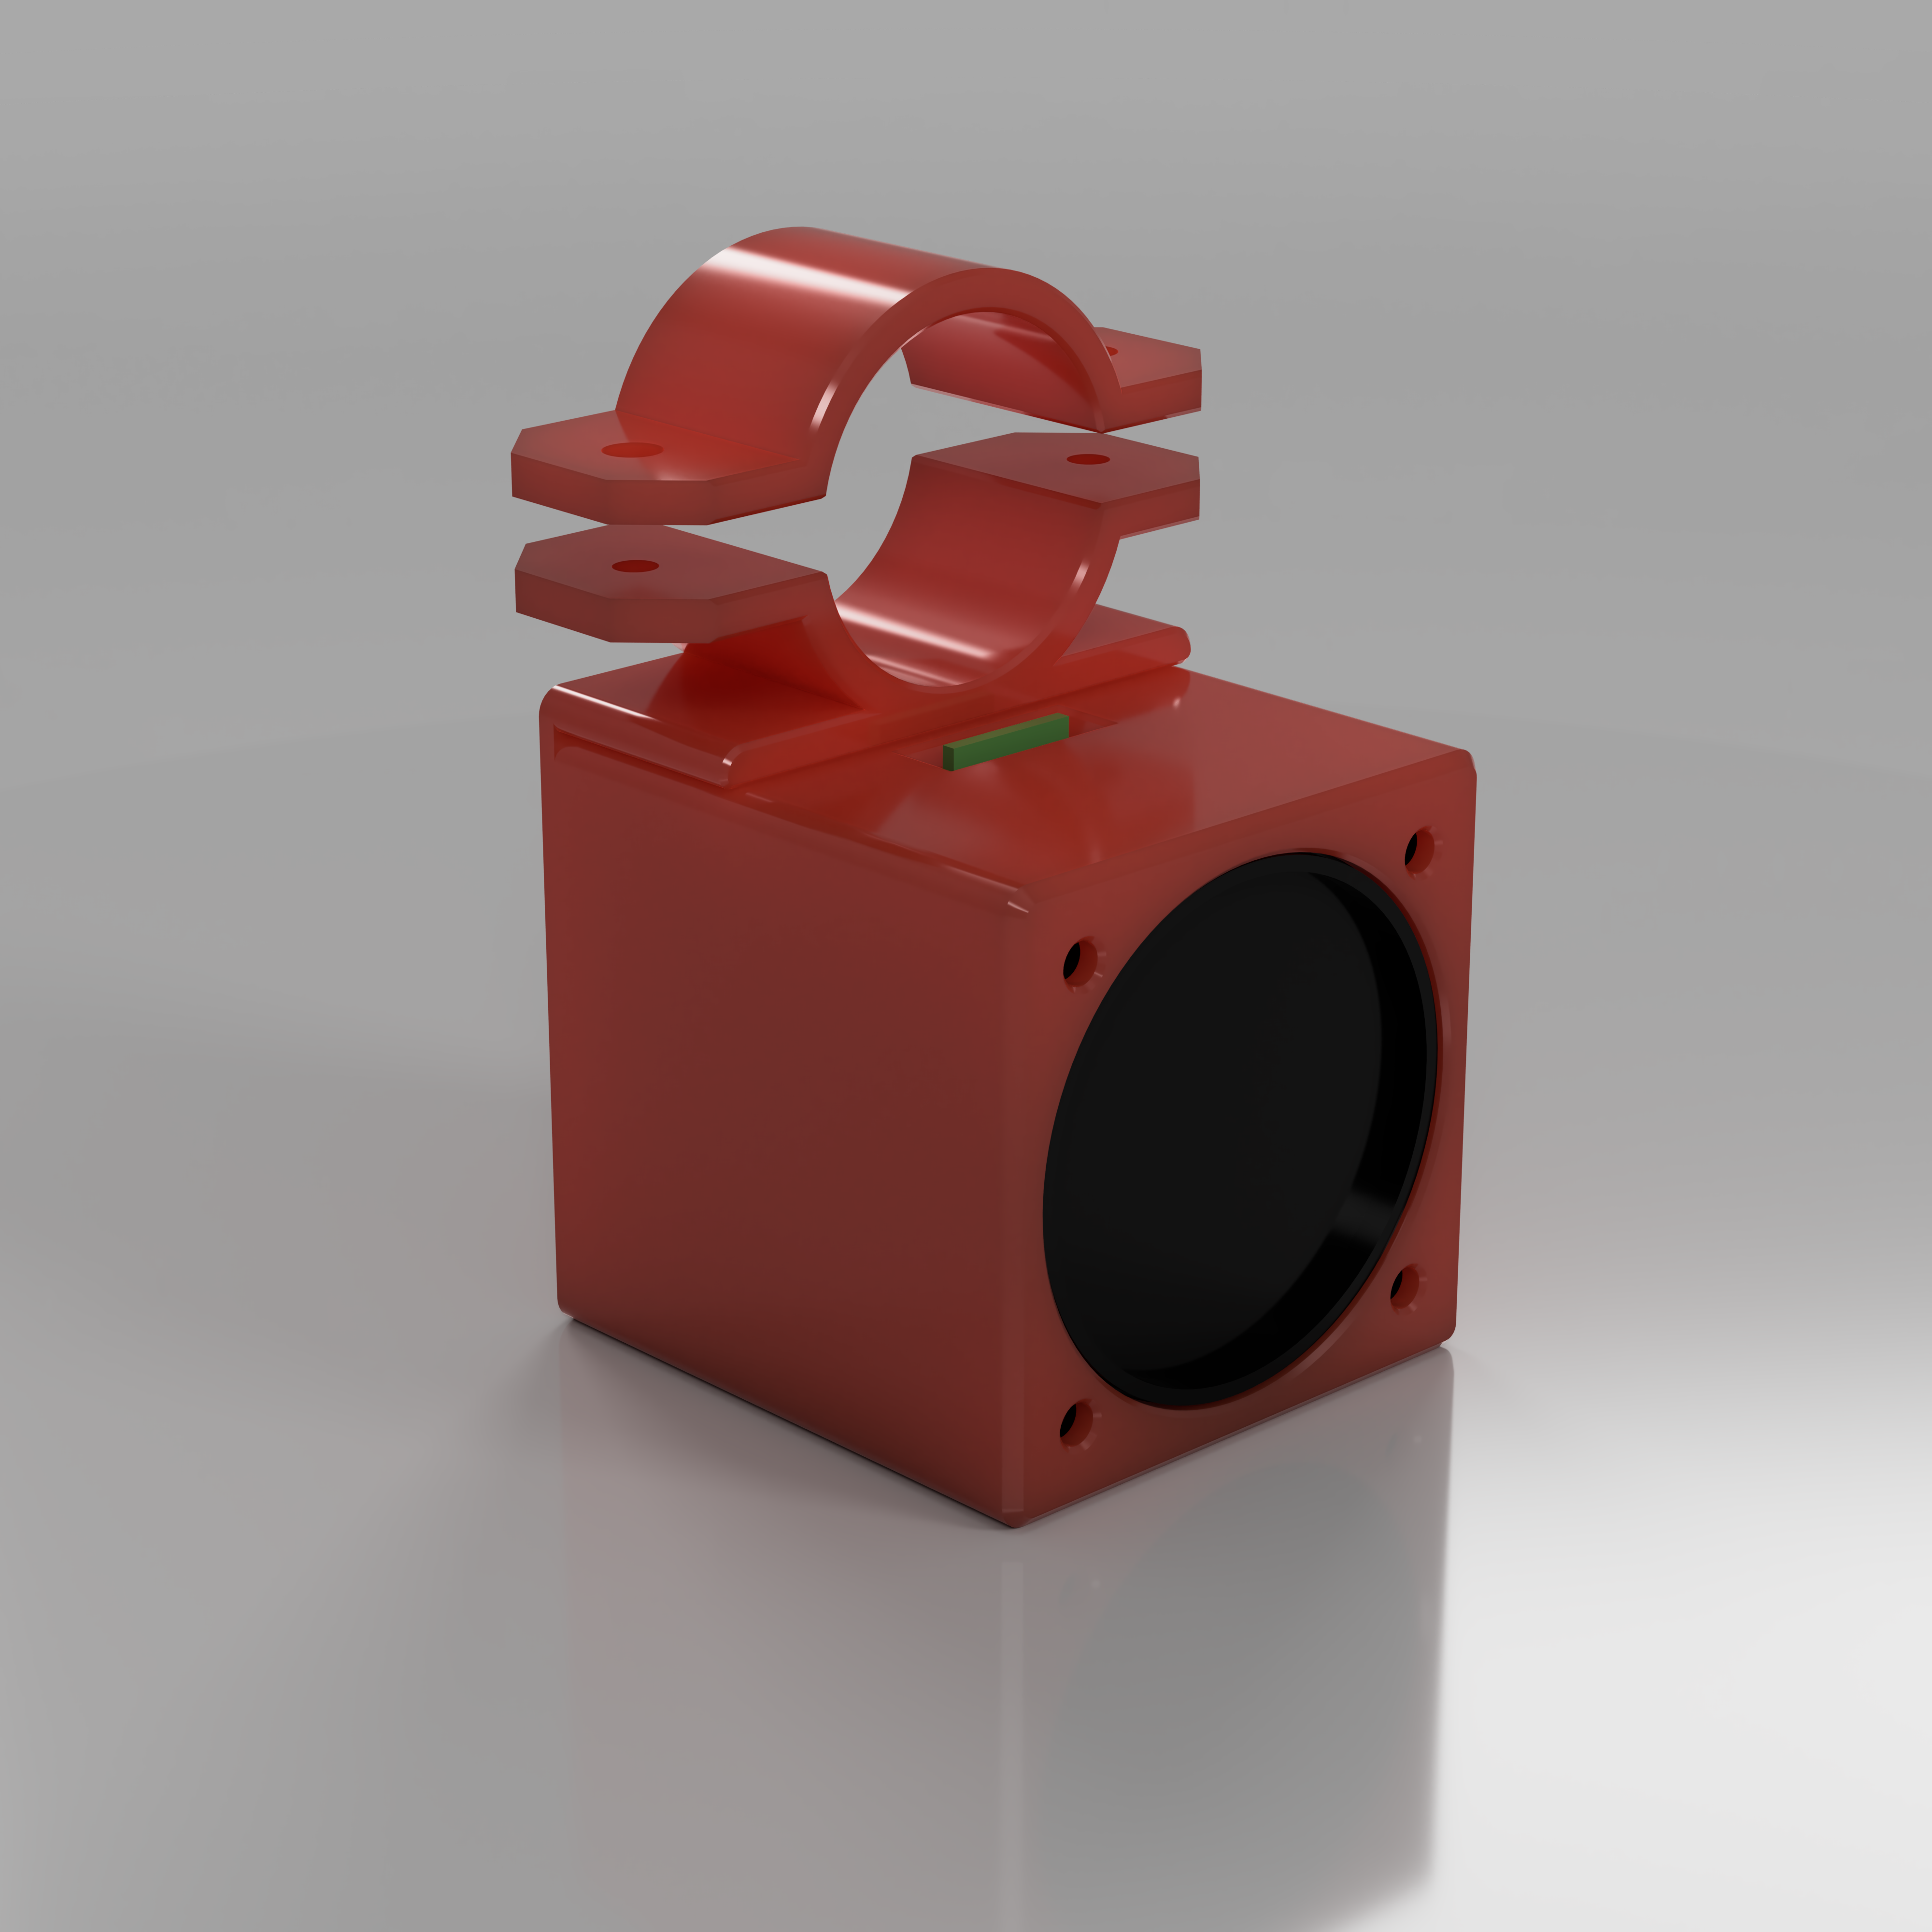
\includegraphics[width=.8\linewidth]{graphics/cad/walkingaid_1.png}
  \captionsetup{width=0.8\linewidth, justification=centering}
  \centering
  \captionof{figure}{Assembled walking aid device}
  \label{fig:walkingaid_1}
\end{minipage}%
\begin{minipage}{.5\textwidth}
  \centering
  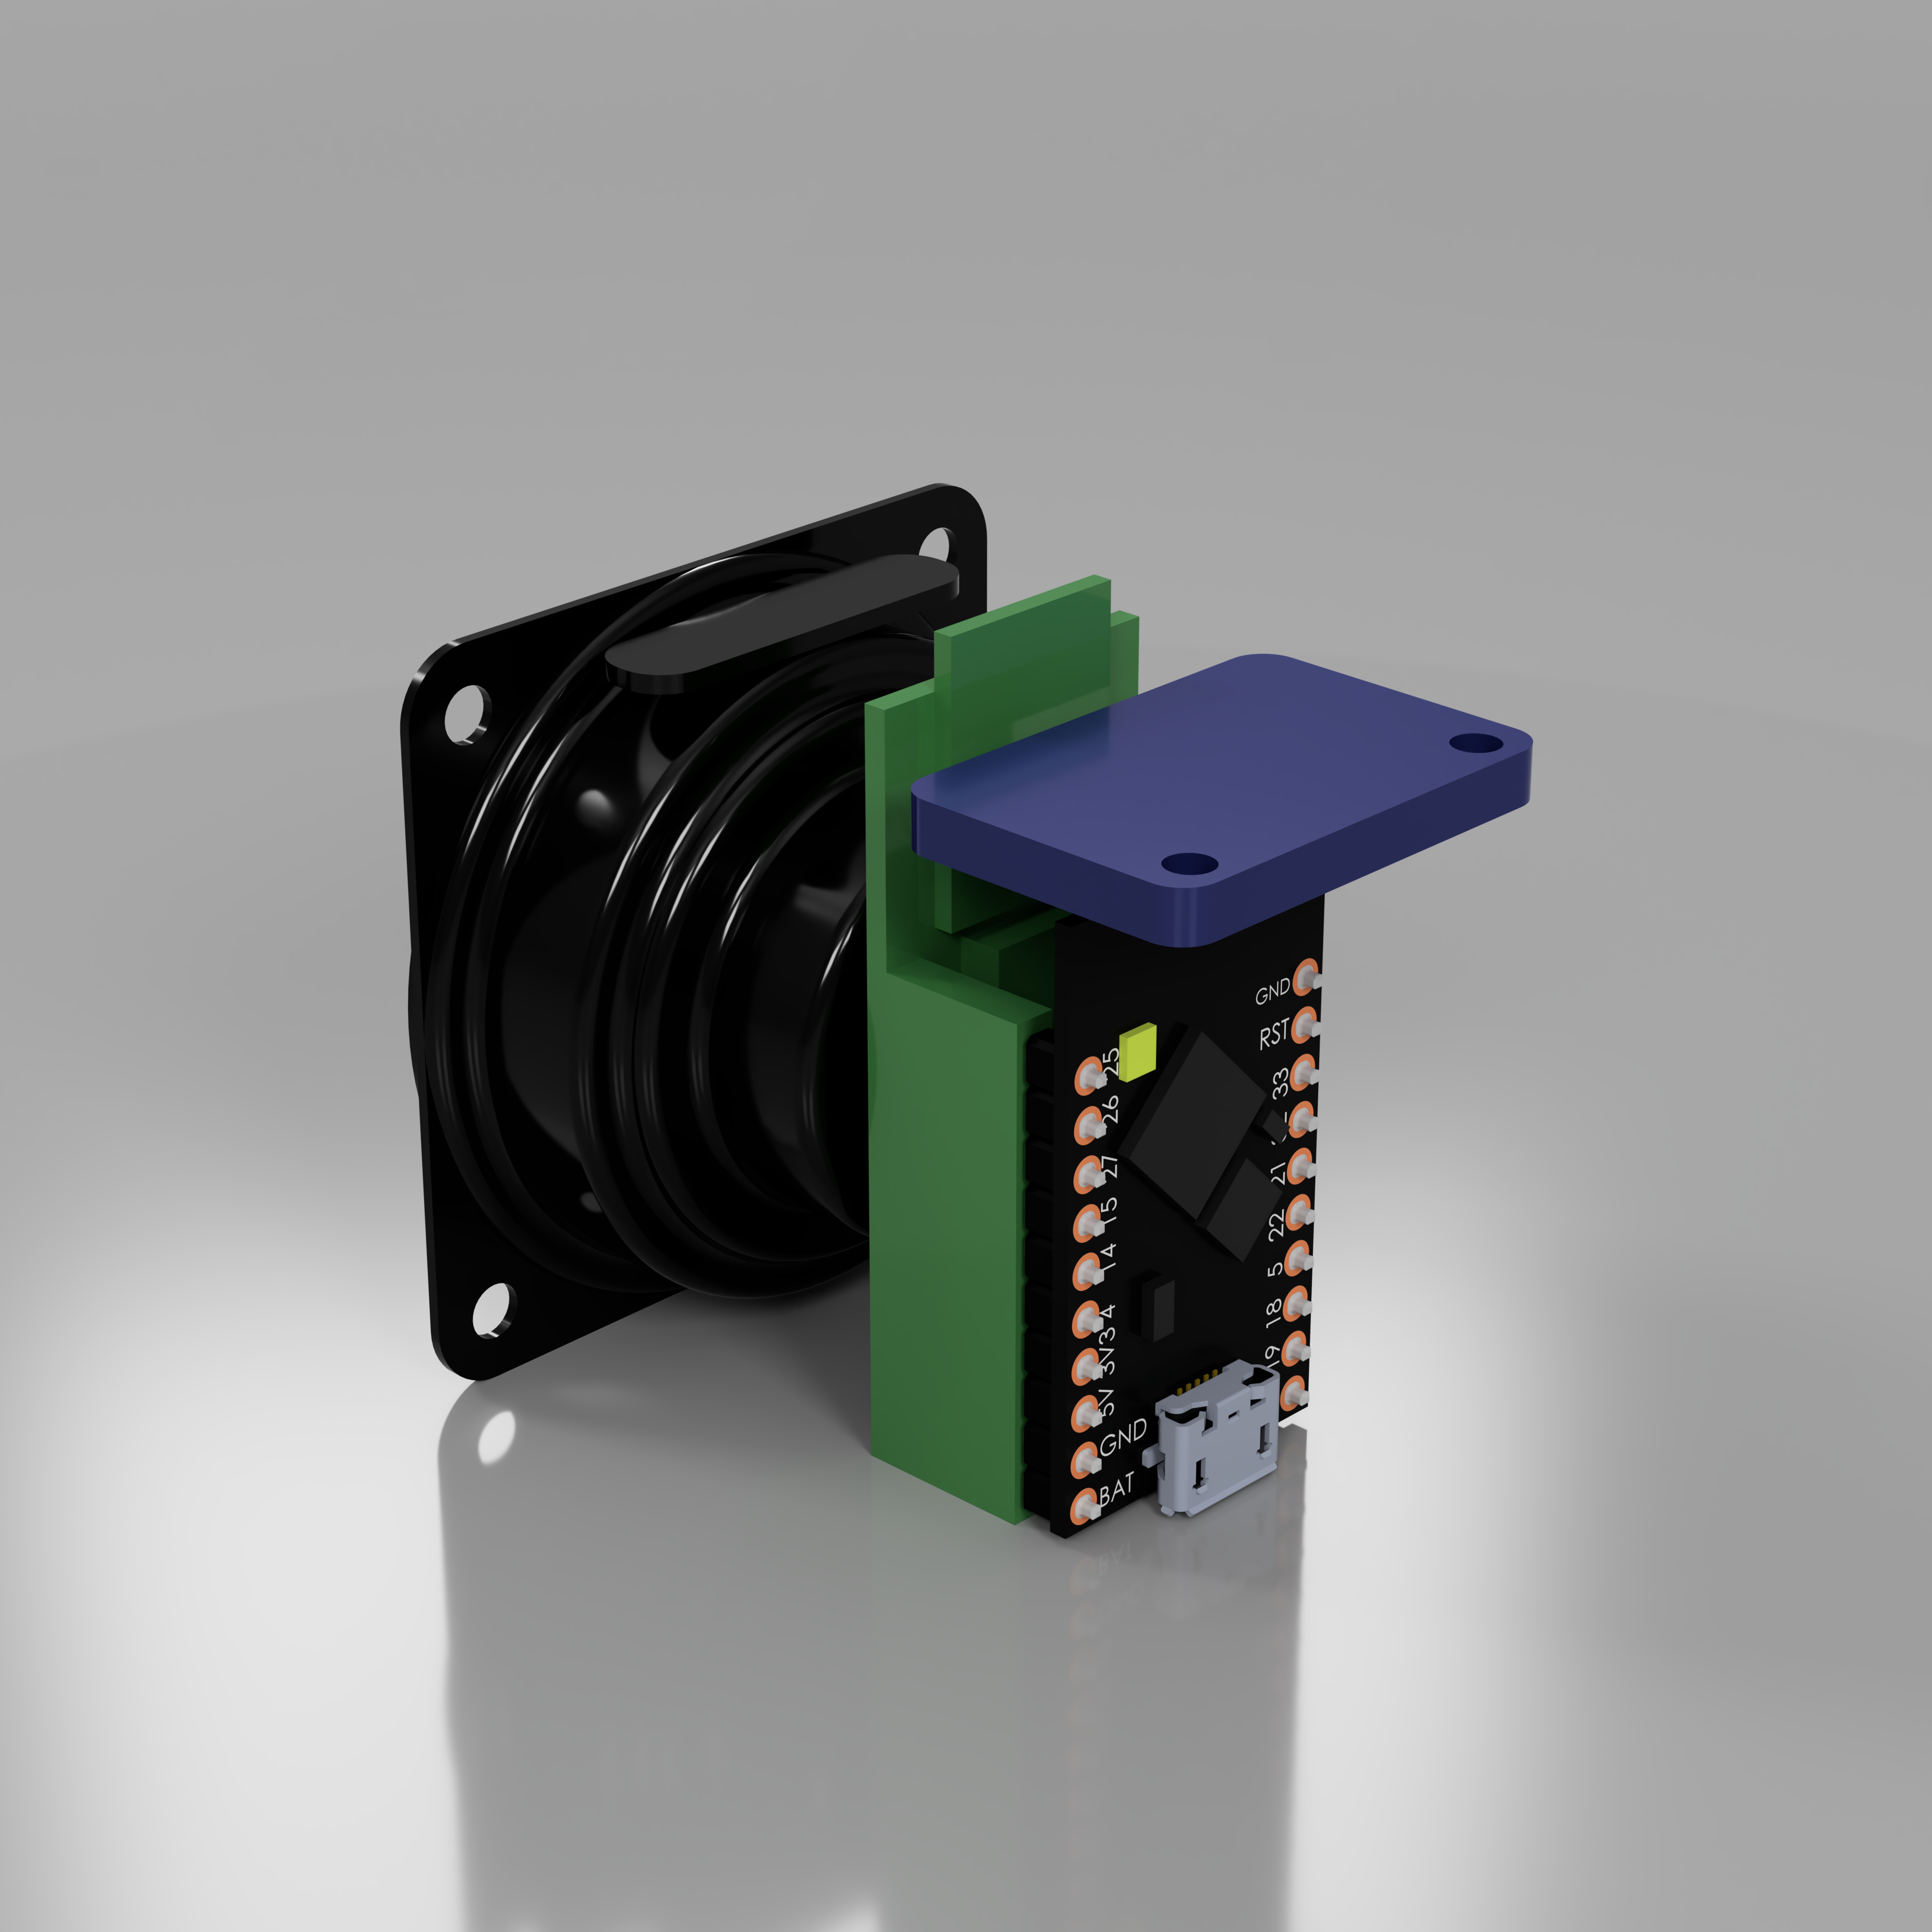
\includegraphics[width=.8\linewidth]{graphics/cad/walkingaid_components_1.png}
  \captionsetup{width=0.8\linewidth, justification=centering}
  \centering
  \captionof{figure}{Walking aid device component layout}
  \label{fig:walkingaid_components_1}
\end{minipage}
\end{figure}

            The design was made as modular as possible, to allow for changeable parts, to make it inter-operable different walking aids and mounting/battery options. The mounting options were inspired from the GoPro style of handlebar mount, this was chosen due to its simplicity, and the sturdiness of attachment which will help with the reading from our accelerometers. The mount was scaled down to more appropriately attach to a walking stick or Zimmer frame, but as mentioned can be easily swapped and modified to work with bigger or smaller tubes/frames.

            In order to fulfil the specification, and allow for familiar voices to remind the users, a MicroSD card was chosen as described above. This required easy access to the card slot, which had to be intuitive and accessible without disassembly of the device.

            \begin{figure}[H]
\centering
\begin{minipage}{.5\textwidth}
  \centering
  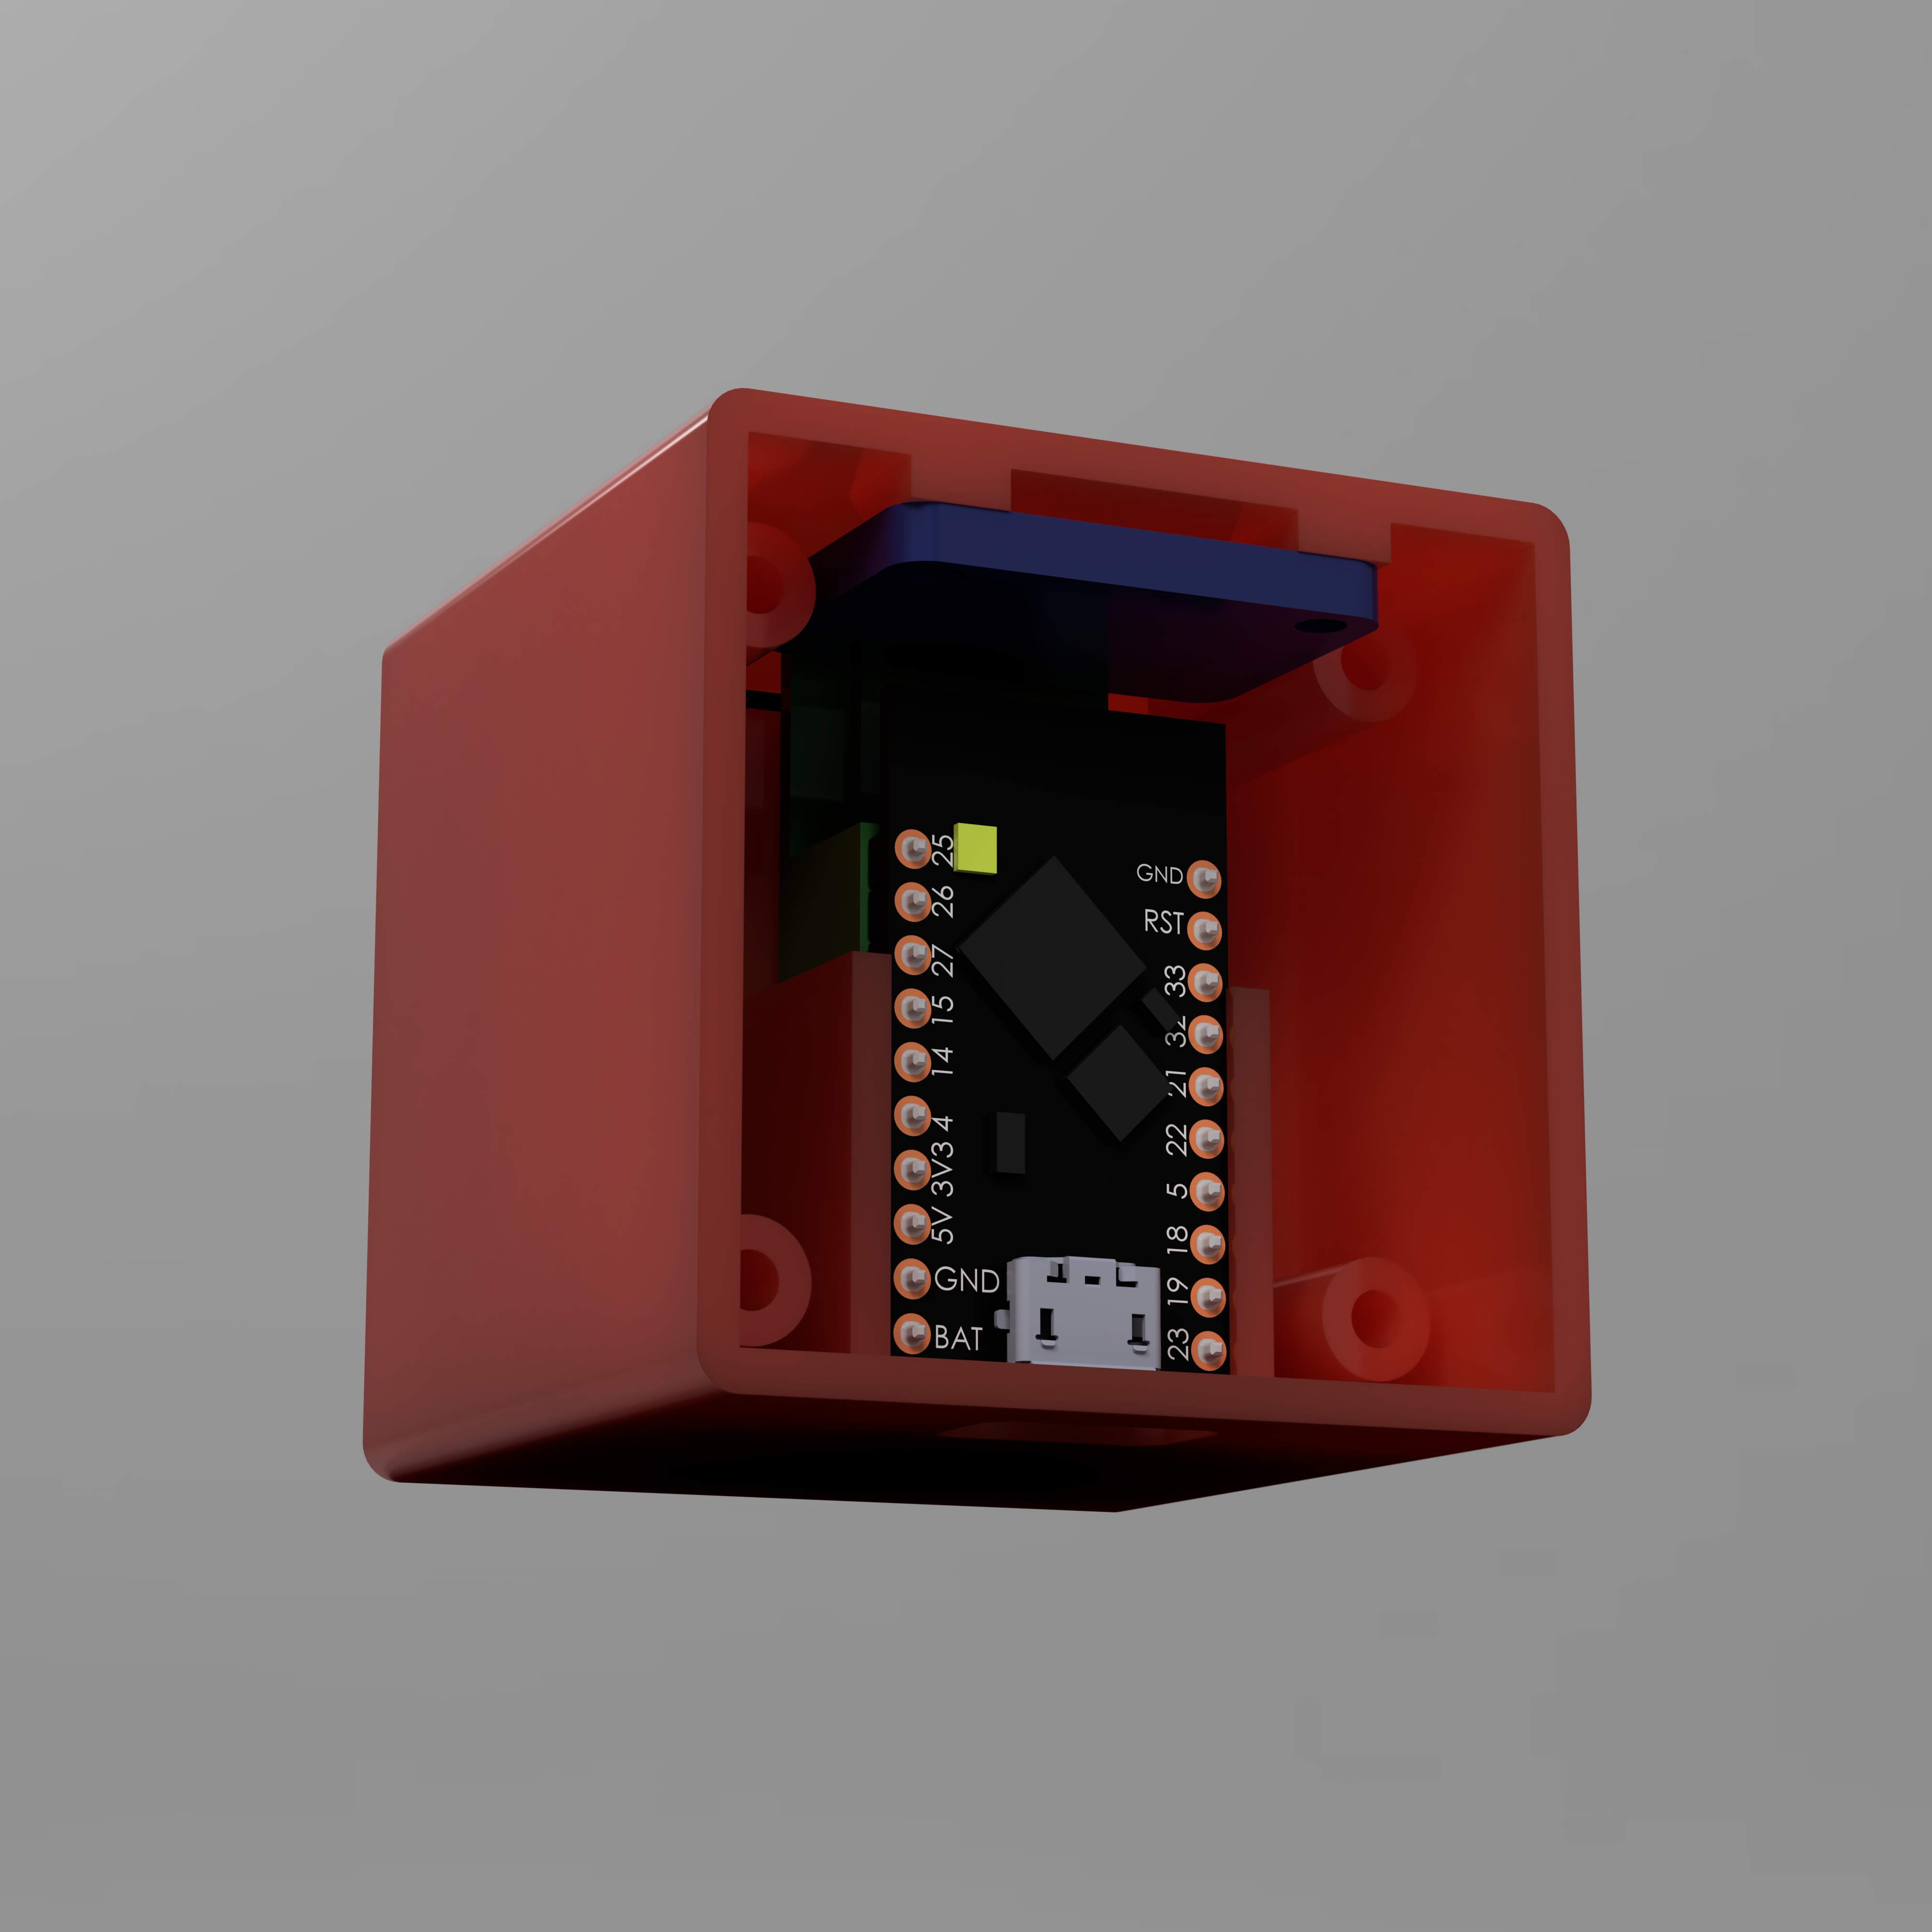
\includegraphics[width=.8\linewidth]{graphics/cad/walkingaid_interior_1.png}
  \captionsetup{width=0.8\linewidth, justification=centering}
  \centering
  \captionof{figure}{Walking aid interior view}
  \label{fig:walkingaid_interior_1}
\end{minipage}%
\begin{minipage}{.5\textwidth}
  \centering
  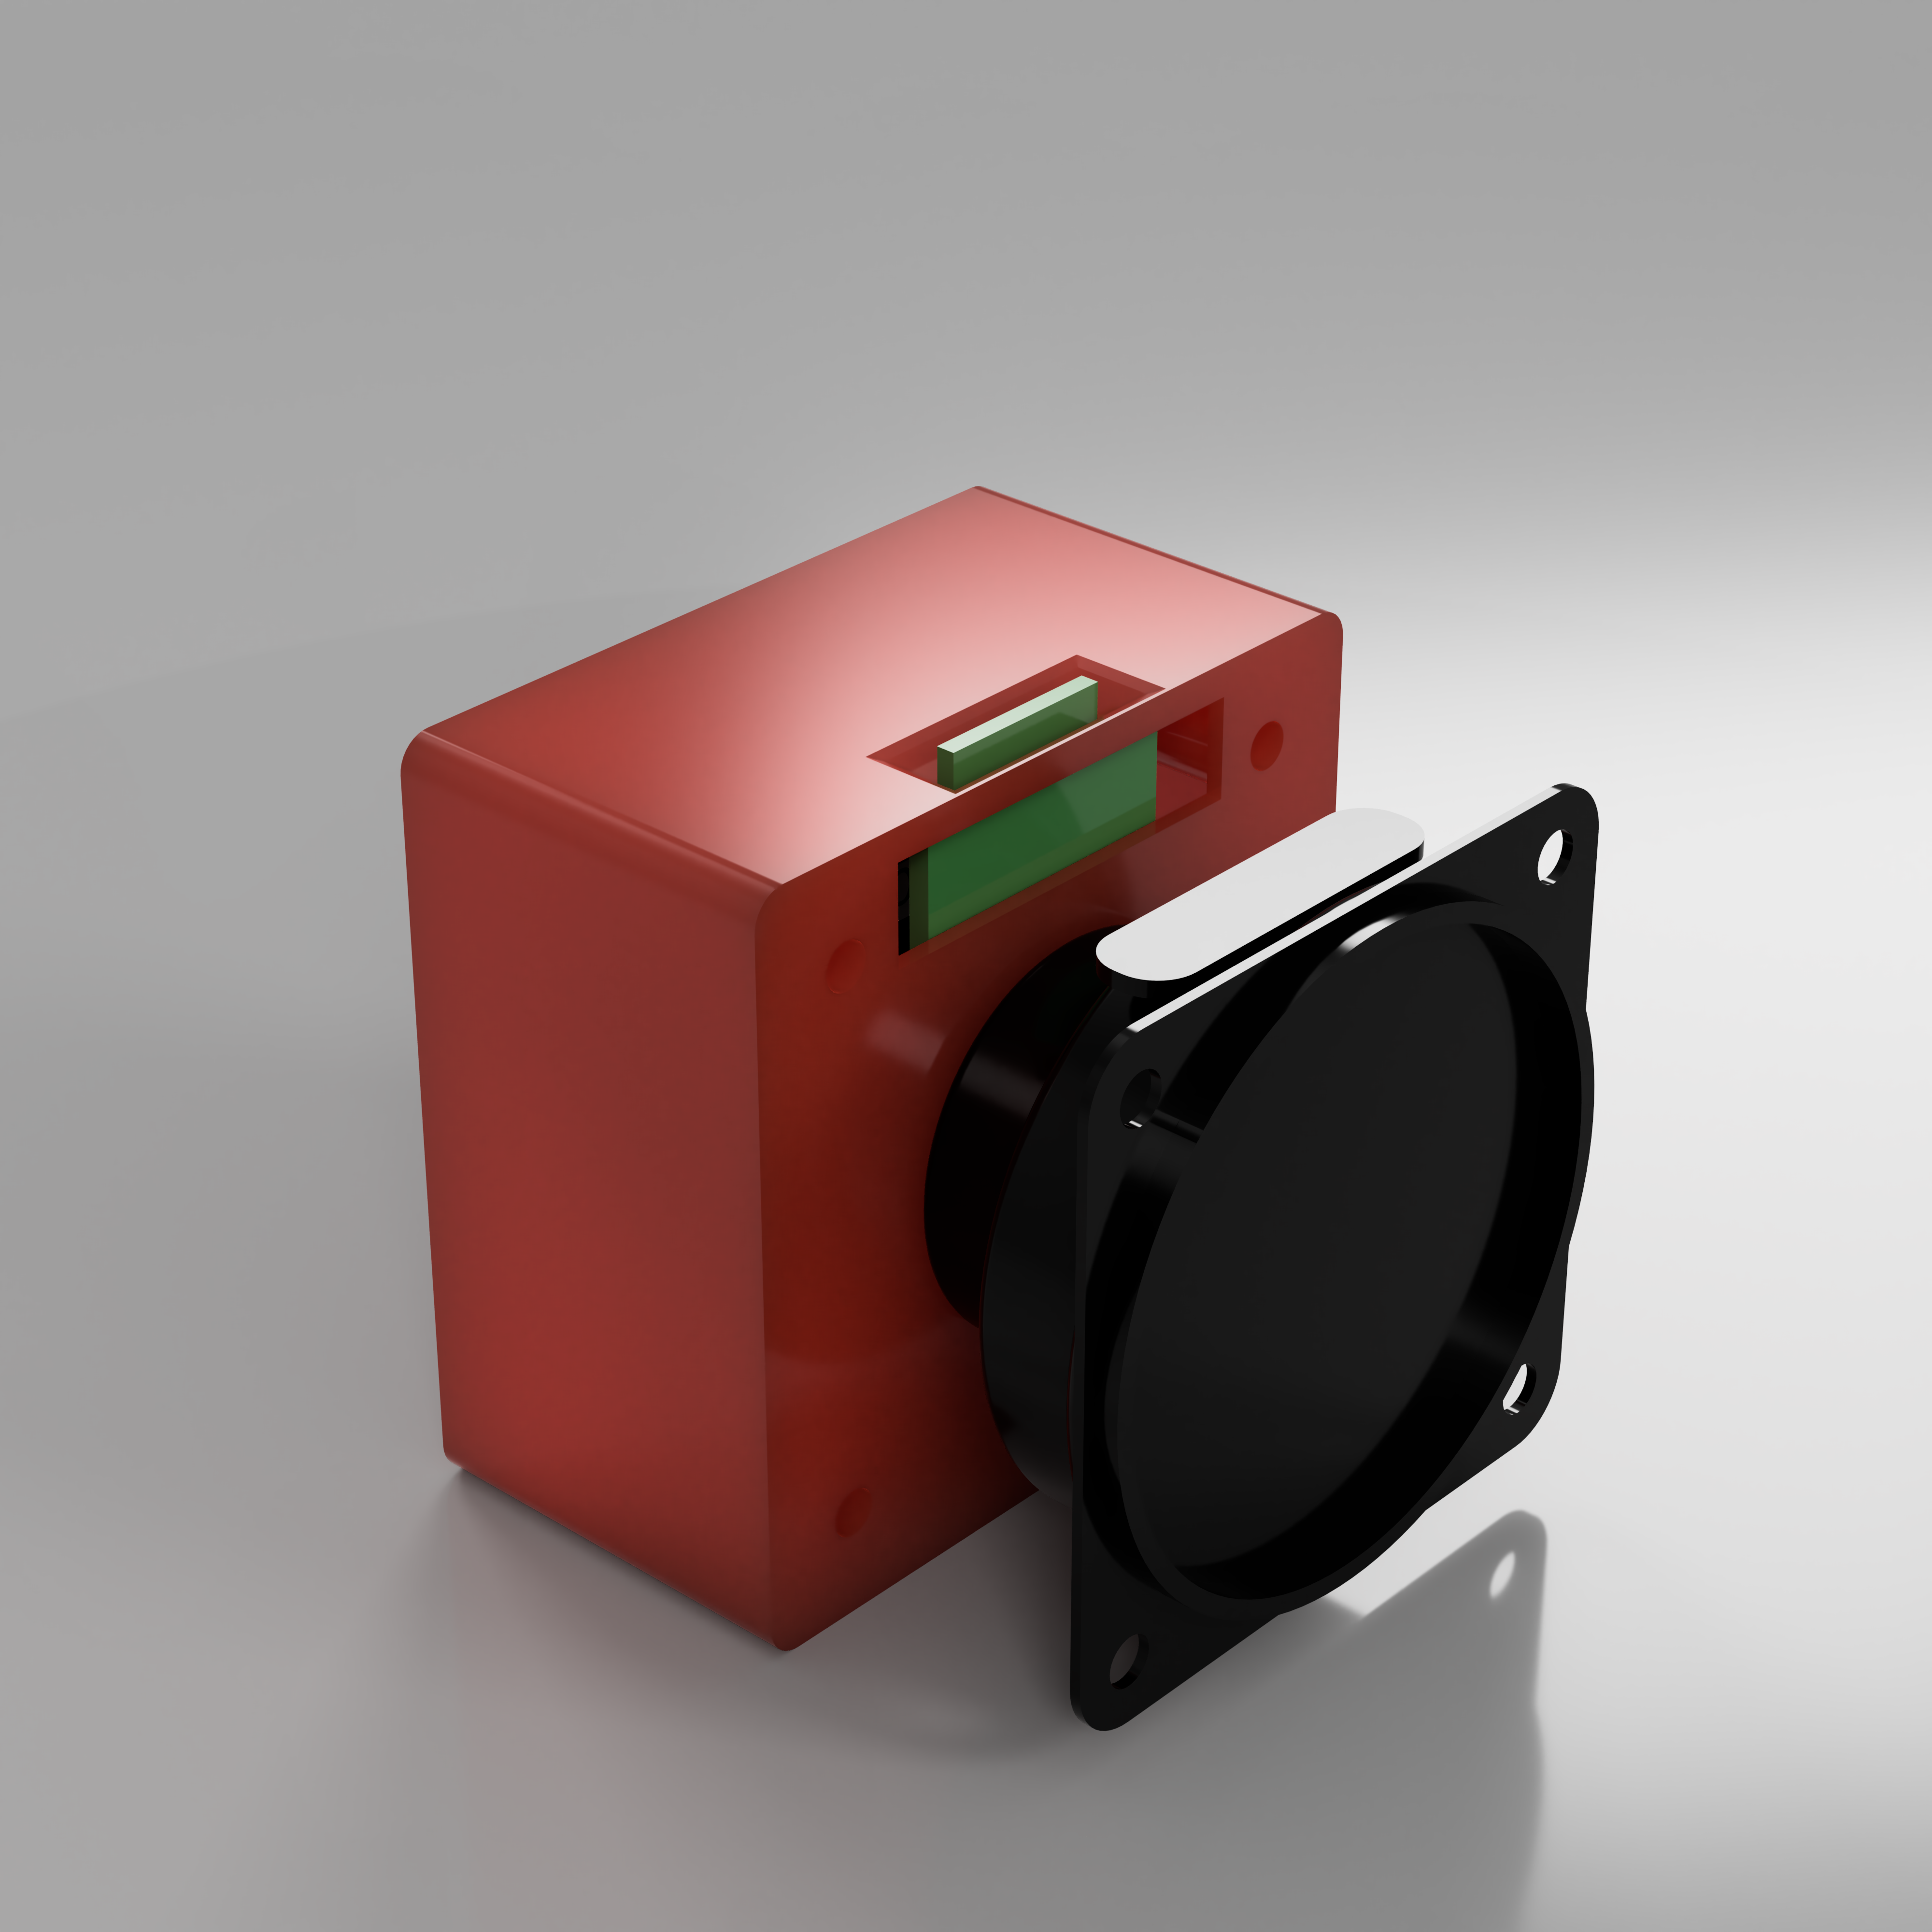
\includegraphics[width=.8\linewidth]{graphics/cad/walkingaid_midhousing_1.png}
  \captionsetup{width=0.8\linewidth, justification=centering}
  \centering
  \captionof{figure}{Walking aid mid housing layout}
  \label{fig:walkingaid_midhousing_1}
\end{minipage}
\end{figure}

            Further considerations include easy access to the microUSB port. This port is required for programming/updating the device, as well as be an option for powering the device if no battery is wanted/needed, or a 5v source is available (such as a large, portable powerbank).

            As noted, the current prototype has no battery support, but the design decision for this walking aid device is to offer swappable endcases, this helps with modularity to allow for different mounts and attachments, but with a through hole for wiring, this allows for future implementations of battery based sources, such as replaceable batteries or rechargeable internal cells.


        \subsection{Prototype}
        \label{subsec:prototype_walking_aid}

            As with the wearable device, assembly was made using standard M3 sized bolts, this time 35mm long to ensure suffcient length to attach the the front and rear endcasing to the midframe. This designed allows assembly to be done rather easily, and again utilising the self-tapping capabilities of the ABS plastic to retain the screws.

            Before assembly, the speaker wires had to be attached to the terminal of the Audio Shield, as the TinyPico would block access to it later on in assembly. The wires had to be fed through the access hole in the midframe, to allow access as well as boost the internal area that the speaker can leverage for stronger sound.

            \begin{figure}[H]
\centering
\begin{minipage}{.5\textwidth}
  \centering
  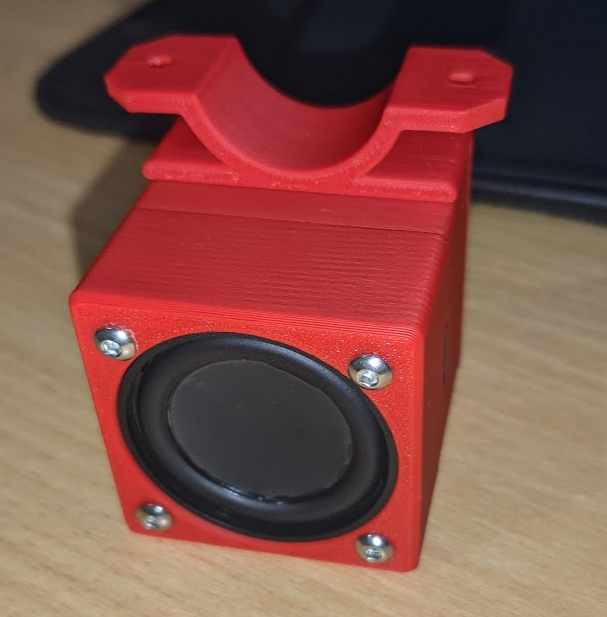
\includegraphics[width=.8\linewidth]{graphics/prototype/walkingaid_1.png}
  \captionsetup{width=0.8\linewidth, justification=centering}
  \centering
  \captionof{figure}{Assembled walking aid device}
  \label{fig:walkingaid_proto_1}
\end{minipage}%
\begin{minipage}{.5\textwidth}
  \centering
  \includegraphics[width=.8\linewidth]{graphics/prototype/walkingaid_hand.jpeg}
  \captionsetup{width=0.8\linewidth, justification=centering}
  \centering
  \captionof{figure}{Assembled walking aid device, shown in hand}
  \label{fig:walkingaid_proto_2}
\end{minipage}
\end{figure}

            The front encases the 40mm driver, and the 4 screws attach it to the midframe securely without further adhesives, initially we had thought that spacers may be needed to stop unnecessary movement, but we instead opted for friction fit tolerances during design, which allowed for this step to be skipped and for an easier assembly process. The original speaker wiring is used, to ensure the correct gauge and rating is used and therefor safe.

            The TinyPico with the accompanying soldered ADXL wiring is then added to the assembly. Side brackets are included in the complex midplate, that stop the boards from moving inside the casing. This is critical as we did not want internal movement to affect the sensitive accelerometer, and due to the SD Card and MicroUSB port requiring precise cutouts in order to remain accessible.

            \begin{figure}[H]
\centering
\begin{minipage}{.5\textwidth}
  \centering
  \includegraphics[width=.8\linewidth]{graphics/prototype/walkingaid_wiring.jpeg}
  \captionsetup{width=0.8\linewidth, justification=centering}
  \centering
  \captionof{figure}{Internal wiring of the walking aid device}
  \label{fig:walkingaid_wiring}
\end{minipage}%
\begin{minipage}{.5\textwidth}
  \centering
  \includegraphics[width=.8\linewidth]{graphics/prototype/walkingaid_rear.jpeg}
  \captionsetup{width=0.8\linewidth, justification=centering}
  \centering
  \captionof{figure}{Rear endcasing of the walking aid device}
  \label{fig:walkingaid_rear}
\end{minipage}
\end{figure}

            The rear endcasing can then be attached, in the same manner as the front casing. This self taps into the designed screw holes, and ensures that both sides of the device are securely clamped and in place.


        \subsection{UML}
        \label{sec:uml_walk_aid}
        
            This section will break down the software systems utilised in the walking aid device into formal language representations. These will take the form of a class diagram, which will illustrate the relationships between each of classes developed for the system, and an activity diagram which will demonstrate the sequence of events that will take place in the system and how they are handled. We hope that this section will help the reader to understand the software system in a broken down, step-by-step manner and to gain an understanding of our rationale towards programming choices that helped us to fulfil the user requirements. The class diagrams will be followed by an explanation of the role of each class and its functions, with the activity diagram also being accompanied by a body of text that establishes in natural language the sequence of events that will take place in the software system and how they are processed.

            \subsubsection{Class Diagram}
            \label{subsubsec:class_diagram_walking_aid}

                To demonstrate how the classes within the software are laid out and how they communicate with one another to make up the whole system, we include here a class diagram. Following the class diagram, we will include documentation on each class and their functions towards benefiting the functionality of the system. 

                \clearpage
                \thispagestyle{empty}
                \begin{landscape}
                    % [H] means put the figure HERE, directly when you input this code.
\begin{figure}[ht!]
	\centering
	\captionsetup{width=1.0\linewidth}

% We set the width of the figure based on the width of one line of text on the page.
% The value can be tuned to any value in [0.0, 1.0] to scale the image while maintaining its aspect ratio.

	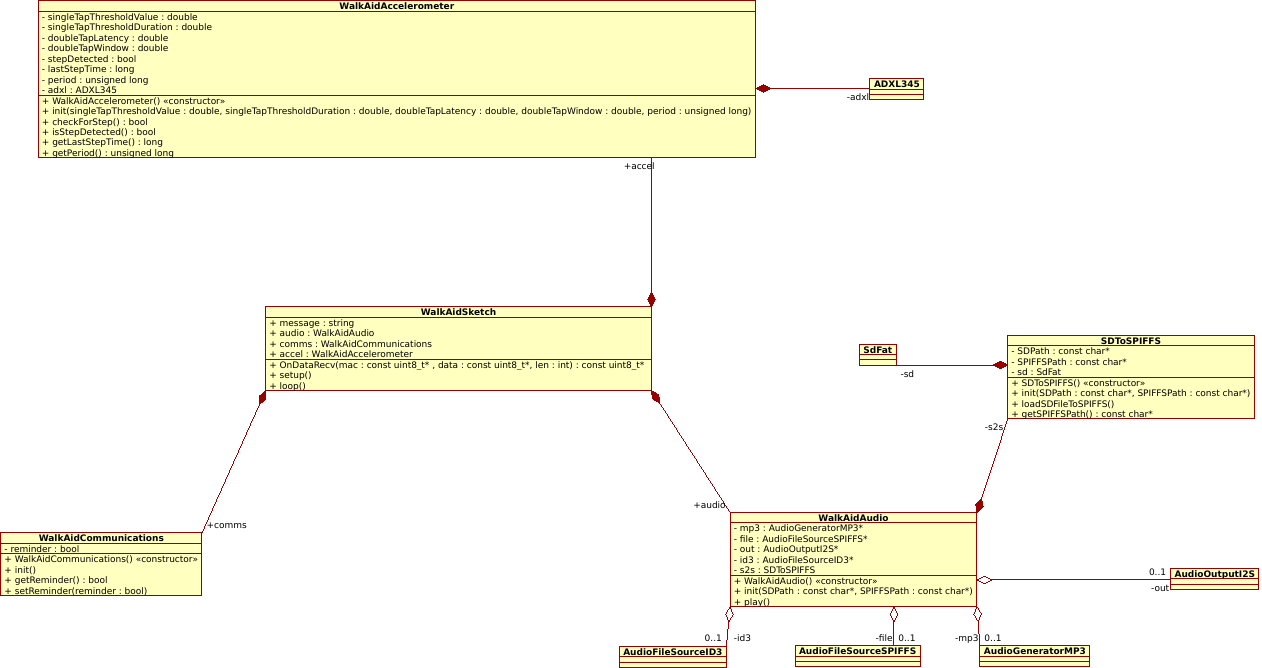
\includegraphics[width=1.0\linewidth]{./UML/WalkingAidDevice/class diagram.png}

% Caption is defined with a short and long version. The short version is shown in the
% List of Figures section, and the long version is used directly with the figure.
	\caption[Walking Aid Device Class Diagram]{A class diagram for the walking aid device software system illustrating how the classes interact with each other.}

% For figures label should be defined after the caption to ensure proper figure numbering.
	\label{fig:class_diagram_walking_aid}

\end{figure}
                \end{landscape}

                \paragraph{WalkAidSketch}\mbox{}

                    This is the main controller of the whole walking aid system and provides the functionality of the setup and loop functions that are required by Arduino systems. It has a composition relationship with the WalkAidAccelerometer, WalkAidCommunications, and the WalkAidAudio classes. Thus, the WalkAidSketch class cannot function without the existence of those classes, and those classes cannot function without the existence of the WalkAidSketch class. The WalkAidSketch class handles the initialisation of the other classes within the setup function, before ensuring that each time the loop function is called, checks are made to see if reminder messages have been received and if so, are responded to accordingly.

                \paragraph{WalkAidAccelerometer}\mbox{}

                    The WalkAidAccelerometer class is responsible for the initialisation of the accelerometer, and the reading of the accelerometer data. The class keeps track of when a step was last taken to avoid the audio reminder being played if the walking aid is moving. It has a composition relationship with the ADXL345 class meaning that neither class could function properly without the existence of each other. This class also relies on the existence of the WalkAidSketch to exist itself.

                \paragraph{WalkAidCommunications}\mbox{}

                    The WalkAidCommunications class is responsible for the initialisation of the ESP-Now communication protocol to establish a connection to the wearable device. When a reminder message is received, the reminder variable is set to true to allow the WalkAidSketch to check for a step in the previous period of time or in the future period of time. Should a reminder need to be played but the user is deaf, this class will send a message back to the wearable device prompting it to vibrate. This class is initialised in the WalkAidSketch class and does not exist unless that class exists. Therefore, it is part of a composition relationship with the WalkAidSketch.

                    The WalkAidCommunications class also makes use of the DebugLED class to ensure that the user is notified of any issues in initialising the communications protocol on boot. It has a composition relationship with the DebugLED class to allow for the LED to be configured should an error occur with the initiation of the communication protocol.

                \paragraph{DebugLED}\mbox{}

                    The DebugLED class exists to handle the configuration of the TinyPICO's onboard LED to indicate whether the communication protocol is working or not. It is initialised in the WearableDeviceSketch class and is therefore part of a composition relationship with the WearableCommunications class. More specifically, an instance of the DebugLED class cannot exist without an instance of the WearableCommunications class.

                    The DebugLED class also holds a composition relationship with the TinyPICO helper library to allow for the configuration of the LED.

                \paragraph{WalkAidAudio}\mbox{}

                    This class handles the initialisation of the SDToSPIFFS class to allow for the transferring of an audio SD file to the SPIFFS memory. Afterwards, it initialises all the necessary classes to interpret the mp3 audio file and play it. This class creates pointers to the AudioFileSourceID3, AudioFileSourceSPIFFS, AudioGeneratorMP3, and AudioOutputI2S classes. It has an aggregation relationship with these classes as it is responsible for their deletion due to them being pointer variables. It also holds a composition relationship with the SDToSPIFFS class, which is utilised for the transferring of the audio file from the SD card to the SPIFFS storage. 

                \paragraph{SDToSPIFFS}\mbox{}

                    This class is responsible only for the transferring of the SD card audio file to the SPIFFS storage. It is part of a composition relationship with the WalkAidAudio class, due to it relying on being initialised in that class to exist. It also holds a composition relationship with the SdFat class, which we discussed in section \ref{subsec:sdfat}, to handle the more intricate SD card functions. 
                
                \newpage

            \subsubsection{Activity Diagram}
            \label{subsubsec:walking_aid_activity}

                The following is an activity diagram that demonstrates the workflow of the walking aid software system. It demonstrates in a graphical way how the system operates in a step-by-step manner. Accompanying the activity diagram will be a body of text that will describe the overview of the activity diagram in natural language.

                % [H] means put the figure HERE, directly when you input this code.
\begin{figure}[H]
	\centering
	\captionsetup{width=1.0\linewidth}

% We set the width of the figure based on the width of one line of text on the page.
% The value can be tuned to any value in [0.0, 1.0] to scale the image while maintaining its aspect ratio.

	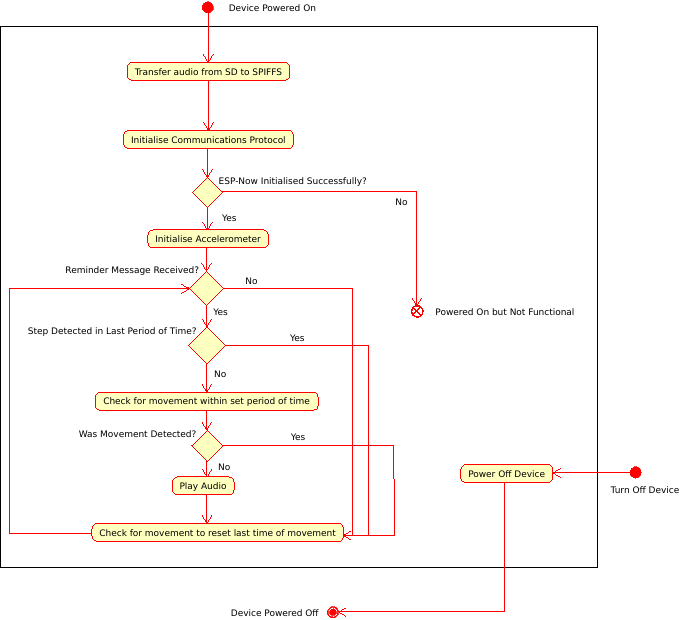
\includegraphics[width=1.0\linewidth]{./UML/WalkingAidDevice/activity diagram.png}

% Caption is defined with a short and long version. The short version is shown in the
% List of Figures section, and the long version is used directly with the figure.
	\caption[Walking Aid Device Activity Diagram]{An activity diagram for the walking aid device software system illustrating the workflow of the system.}

% For figures label should be defined after the caption to ensure proper figure numbering.
	\label{fig:activity_diagram_walking_aid}

\end{figure}
            
                The system begins as soon as the device is powered on. The first process that the system runs is the transferral of the SD audio file to the SPIFFS storage location for quicker access later on. If an error is detected with the process of transferring the audio file from SD card to SPIFFS, then system is left in a non-functional state. The system then attempts to initialise the ESP-Now communication with the wearable device. If this is unsuccessful then it will sit in an inactive state. Otherwise, it will attempt to initialise the accelerometer and begin the loop function of the sketch. 

                For each pass of the loop function, the system firstly checks to see if a reminder message has been received from the wearable device. This message basically states, ``The wearable device is moving, is the walking aid device moving also?''. At this stage, the system checks if the time of the last detected step happened within the last developer set period of time. If a step had been detected in that time, then we skip to the end of the loop and check again for movement in the walking aid to update the last time a movement was detected. Otherwise, we then run a loop for the developer set period of time to check if movement is then detected. This allows the user time to get to their walking aid before having a reminder played or a vibration played through the wearable device. If movement was not detected in that period of time, then we play the audio reminder or send a vibrate message to the wearable device if the user is deaf. If movement was detected then we skip playing the audio or sending a vibrate message and move to the end of the loop. In all instances, the end of the loop signifies that the check for movement should occur again. As previously stated, this is to update the timestamp of the last movement detected. Once this is complete, we move back to the check for reminder message step to start the loop again.

                To terminate the execution of the system prematurely, the device can be powered off. We may not have followed the etiquette of activity diagrams to demonstrate this, but we wanted to demonstrate that the system remains functional in a constant loop unless the device is powered off. We added a second initial activity of turn off device to demonstrate this, where a power off device activity is run and we finish in a state where the device is powered off and non-functional.
            
    \section{Wearable Device}
    \label{sec:wearabledevice}

        The wearable device is one that can be worn on the limbs of the patients to identify when the patient has begun walking. When walking is detected, communication occurs between the walking aid and wearable device to identify if the walking aid device is moving also. 

        \subsection{Walking Detection Technique - Single-Tap Detection}
        \label{subsec:walking_detection_technique}

           With the movement detection of the walking aid device, it was an obvious decision to utilise the single-tap detection feature of the ADXL345 accelerometer. We assume that the walking aid will take the form of a walking stick or Zimmer frame like structure, with movement likely to include lifting and placing. The placing event will cause a change in gravity through the Z-Axis of the accelerometer, and thus will allow the accelerometer to notice a tap being detected.

           The decision of what system to use to detect movement in the wearable device was less simple. Options included using a similar single-tap detection system, a system that utilises changes in acceleration to detect walking, or a system that uses the Bluetooth Low Energy (BLE) technology of each device to measure changes in distances between them. With the option of utilising BLE technology to detect walking, we would have needed to also utilise an accelerometer on one of the devices still to gain an understanding of which device was moving. However, the use of BLE technology for this use case would have been inadequate due to its potential for distance calculation inaccuracies of up to several metres \cite{Fachri_2019}. 

           Therefore, we were left with using the ADXL345 accelerometer for the detection of the user walking. To decide on which solution of accelerometer system to use, we decided to develop both the single-tap detection system and the acceleration change detection system and compare them in real world testing. For our system, the single-tap detection system seemed to work better in attempting to detect walking, where the system attempting to detect changes in acceleration struggled with also detecting any movements in the accelerometer. The single-tap detection system would also be beneficial to us as it would be implementable on both the walking aid and wearable devices. Another benefit to the single-tap detection solution is that it allows versatility as to where the wearable device can be placed, with testing proving that the devices can detect walking on both the user's wrist and their ankle. 

           Ultimately, we decided to implement the single-tap detection system within the wearable device to detect when the user was walking. We make use of a system that checks if the user makes 5 steps within a 10-second period in order to meet the user requirement of reminders only being played if the user has moved over a metre without their walking aid. If they do, then we send a message to the walking aid device to play an audio reminder to the patient to take their walking aid with them if the walking aid device has not detected movement. The main benefits to this system is its versatility to be worn on the user's wrist or ankle, and it provided the foundations to the similar system that has been developed for the walking aid device. In future, we would like to explore the use of the aforementioned ultra-wideband technology (UWB). Due to its distance measurement error being within 10 cm \cite{uwb_accuracy}, it would have been interesting to implement this within the wearable device, and into the walking aid device working in conjunction with an accelerometer to detect if the walking aid is moving.

        \subsection{Physical Design}
        \label{subsec:Design_Decisions_wearable}

            As with the walking aid device, the design was formulated around a minimalistic form factor around the components that needed to be present, in this case, the TinyPico, ADXL, and vibration motor. This prototype needed to be of a particularly small form factor; the client made it clear that patients aren't always happy with new, large and obtrusive objects on their bodies, so the more natural we could make it, the better it would be. This device is very tightly packed, with the components in very short distances of one another, although this could be an issue with electrical shorts, during assembly there will be insulating factors included, that will stop this from happening.

            \begin{figure}[H]
\centering
\begin{minipage}{.5\textwidth}
  \centering
  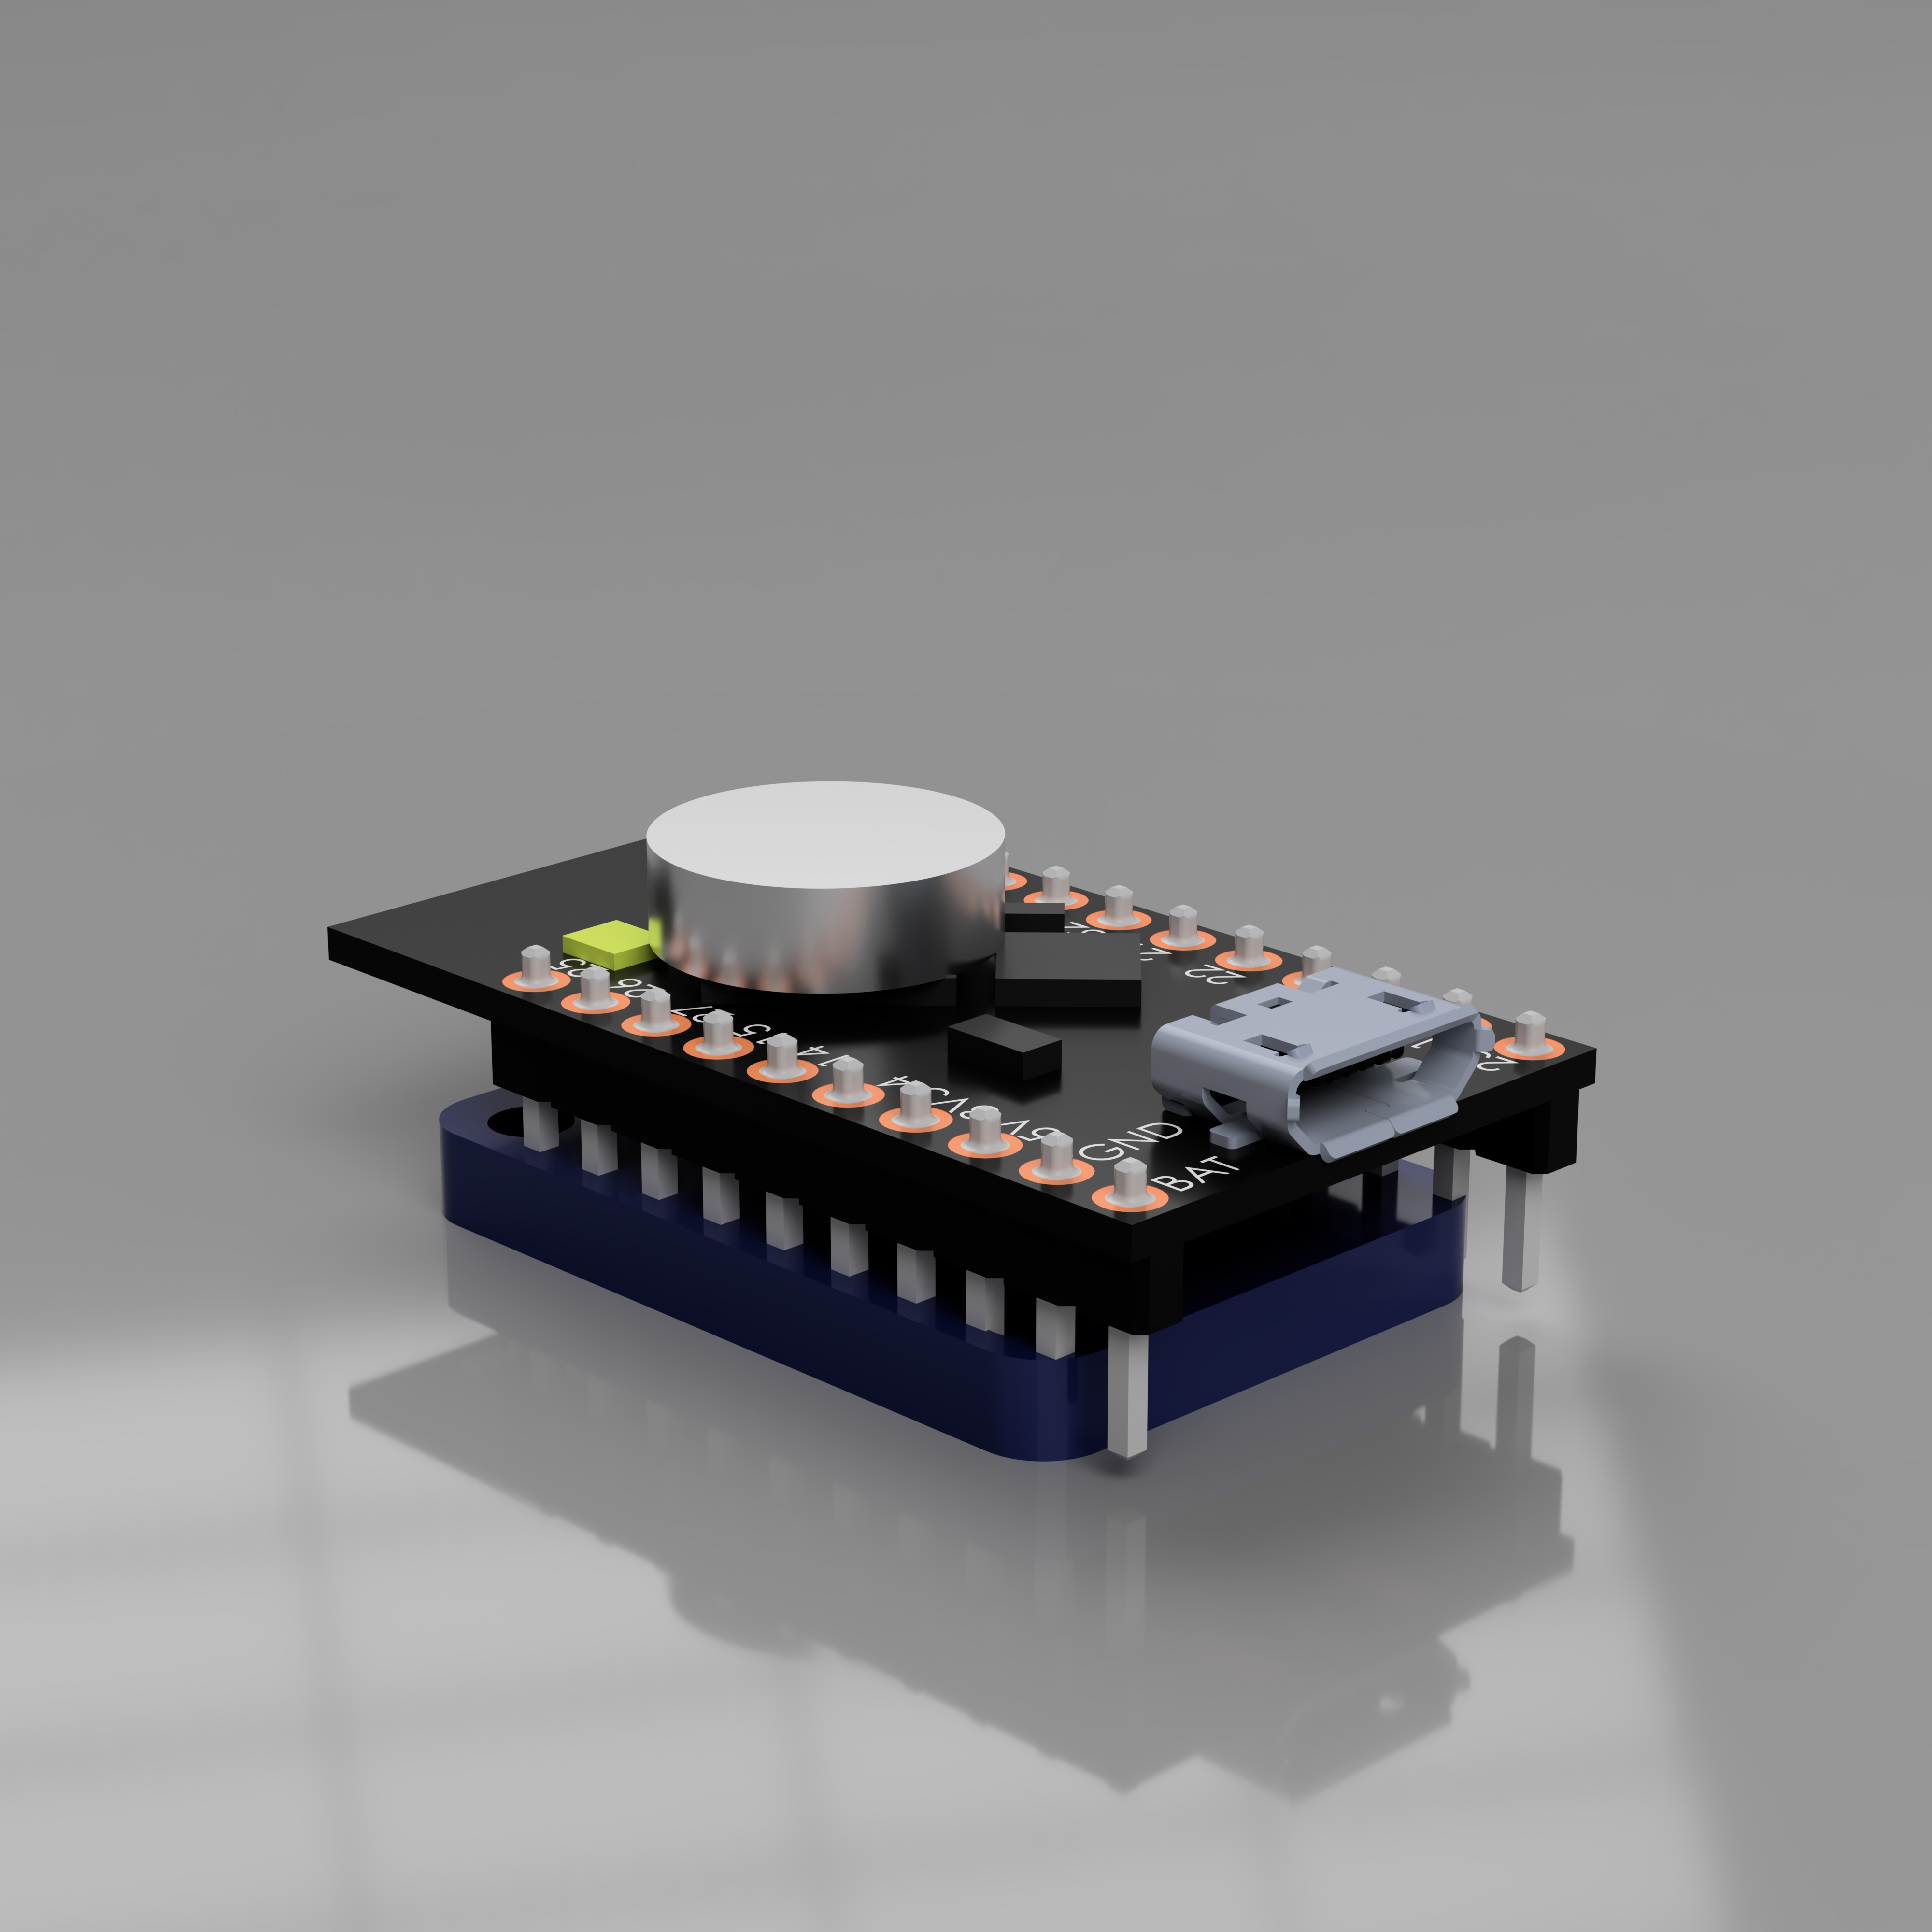
\includegraphics[width=.8\linewidth]{graphics/cad/wearable_components_1.png}
  \captionsetup{width=0.8\linewidth, justification=centering}
  \centering
  \captionof{figure}{Wearable device component layout}
  \label{fig:wearable_components_1}
\end{minipage}%
\begin{minipage}{.5\textwidth}
  \centering
  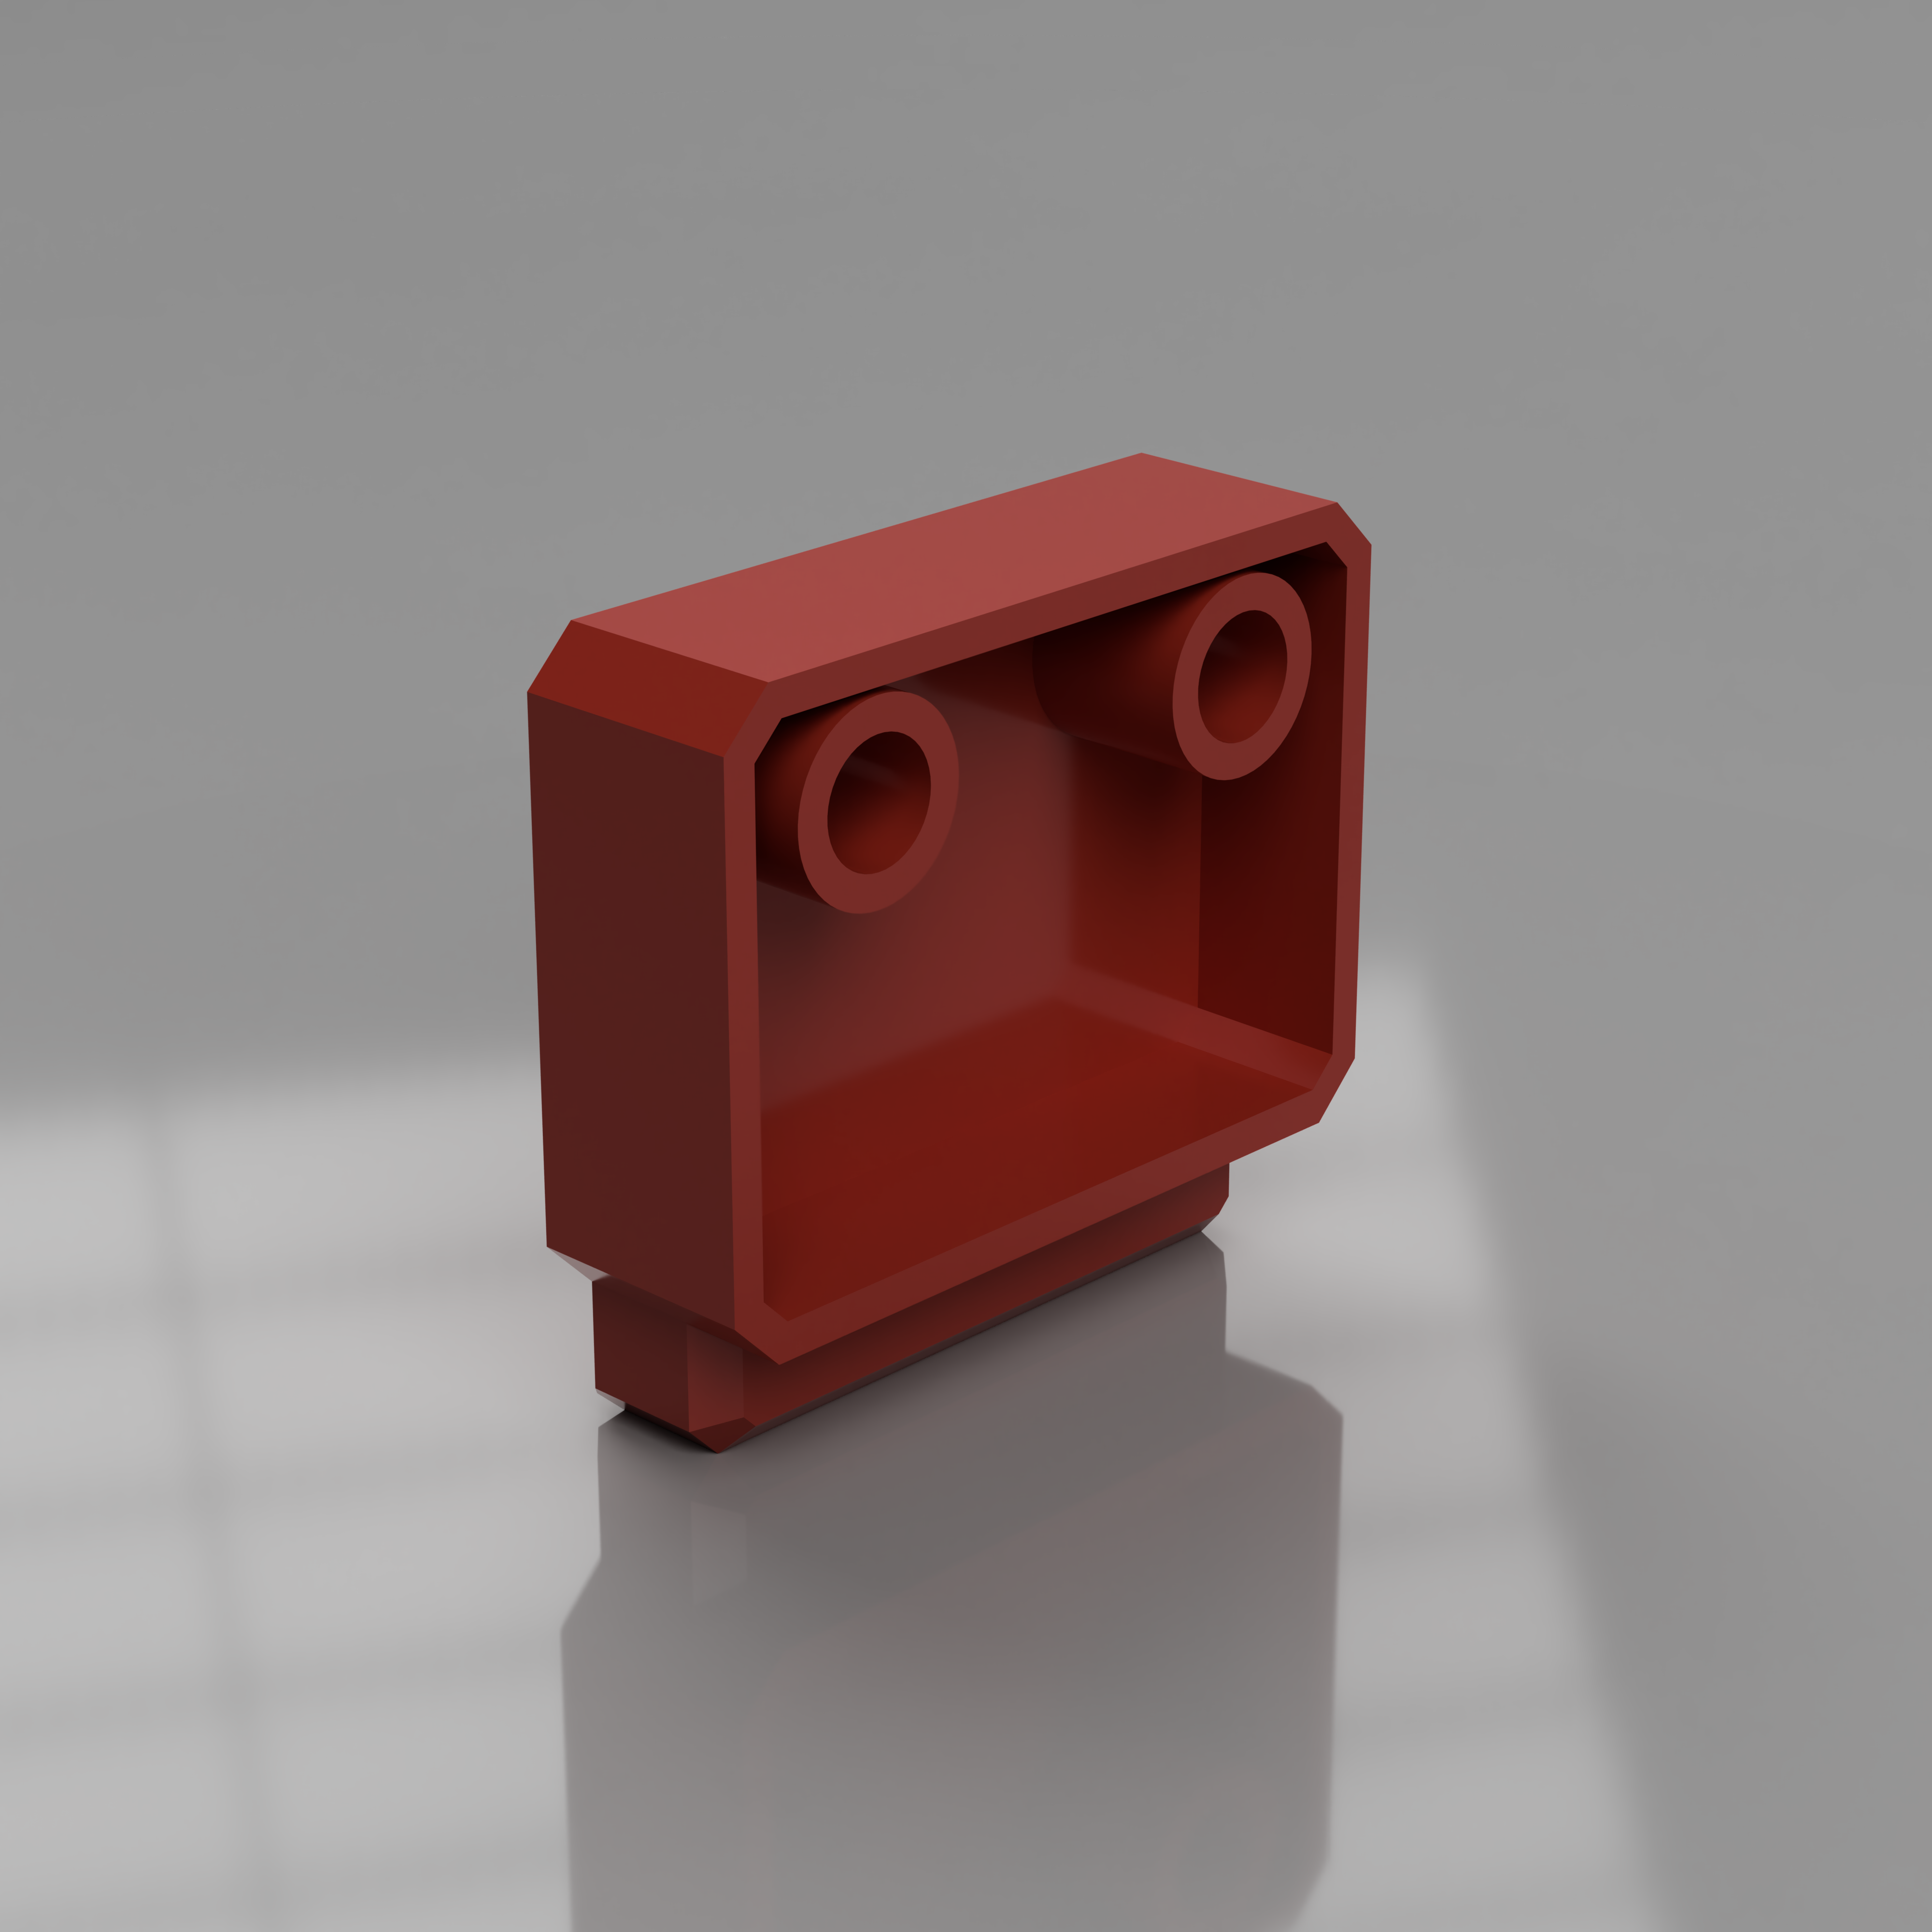
\includegraphics[width=.8\linewidth]{graphics/cad/wearable_endcase_1.png}
  \captionsetup{width=0.8\linewidth, justification=centering}
  \centering
  \captionof{figure}{Walking aid modular end casing}
  \label{fig:walkingaid_endcase_1}
\end{minipage}
\end{figure} %%also includes endcase

            A similar approach was taken regarding the modular design, with an end-housing that can be quickly and easily changed. We designed a base end-plate from which all attachments are based off of, and will include it in the deliverables to ensure the client can adjust and create more as needed from our working template.

            \begin{figure}[H]
\centering
\begin{minipage}{.5\textwidth}
  \centering
  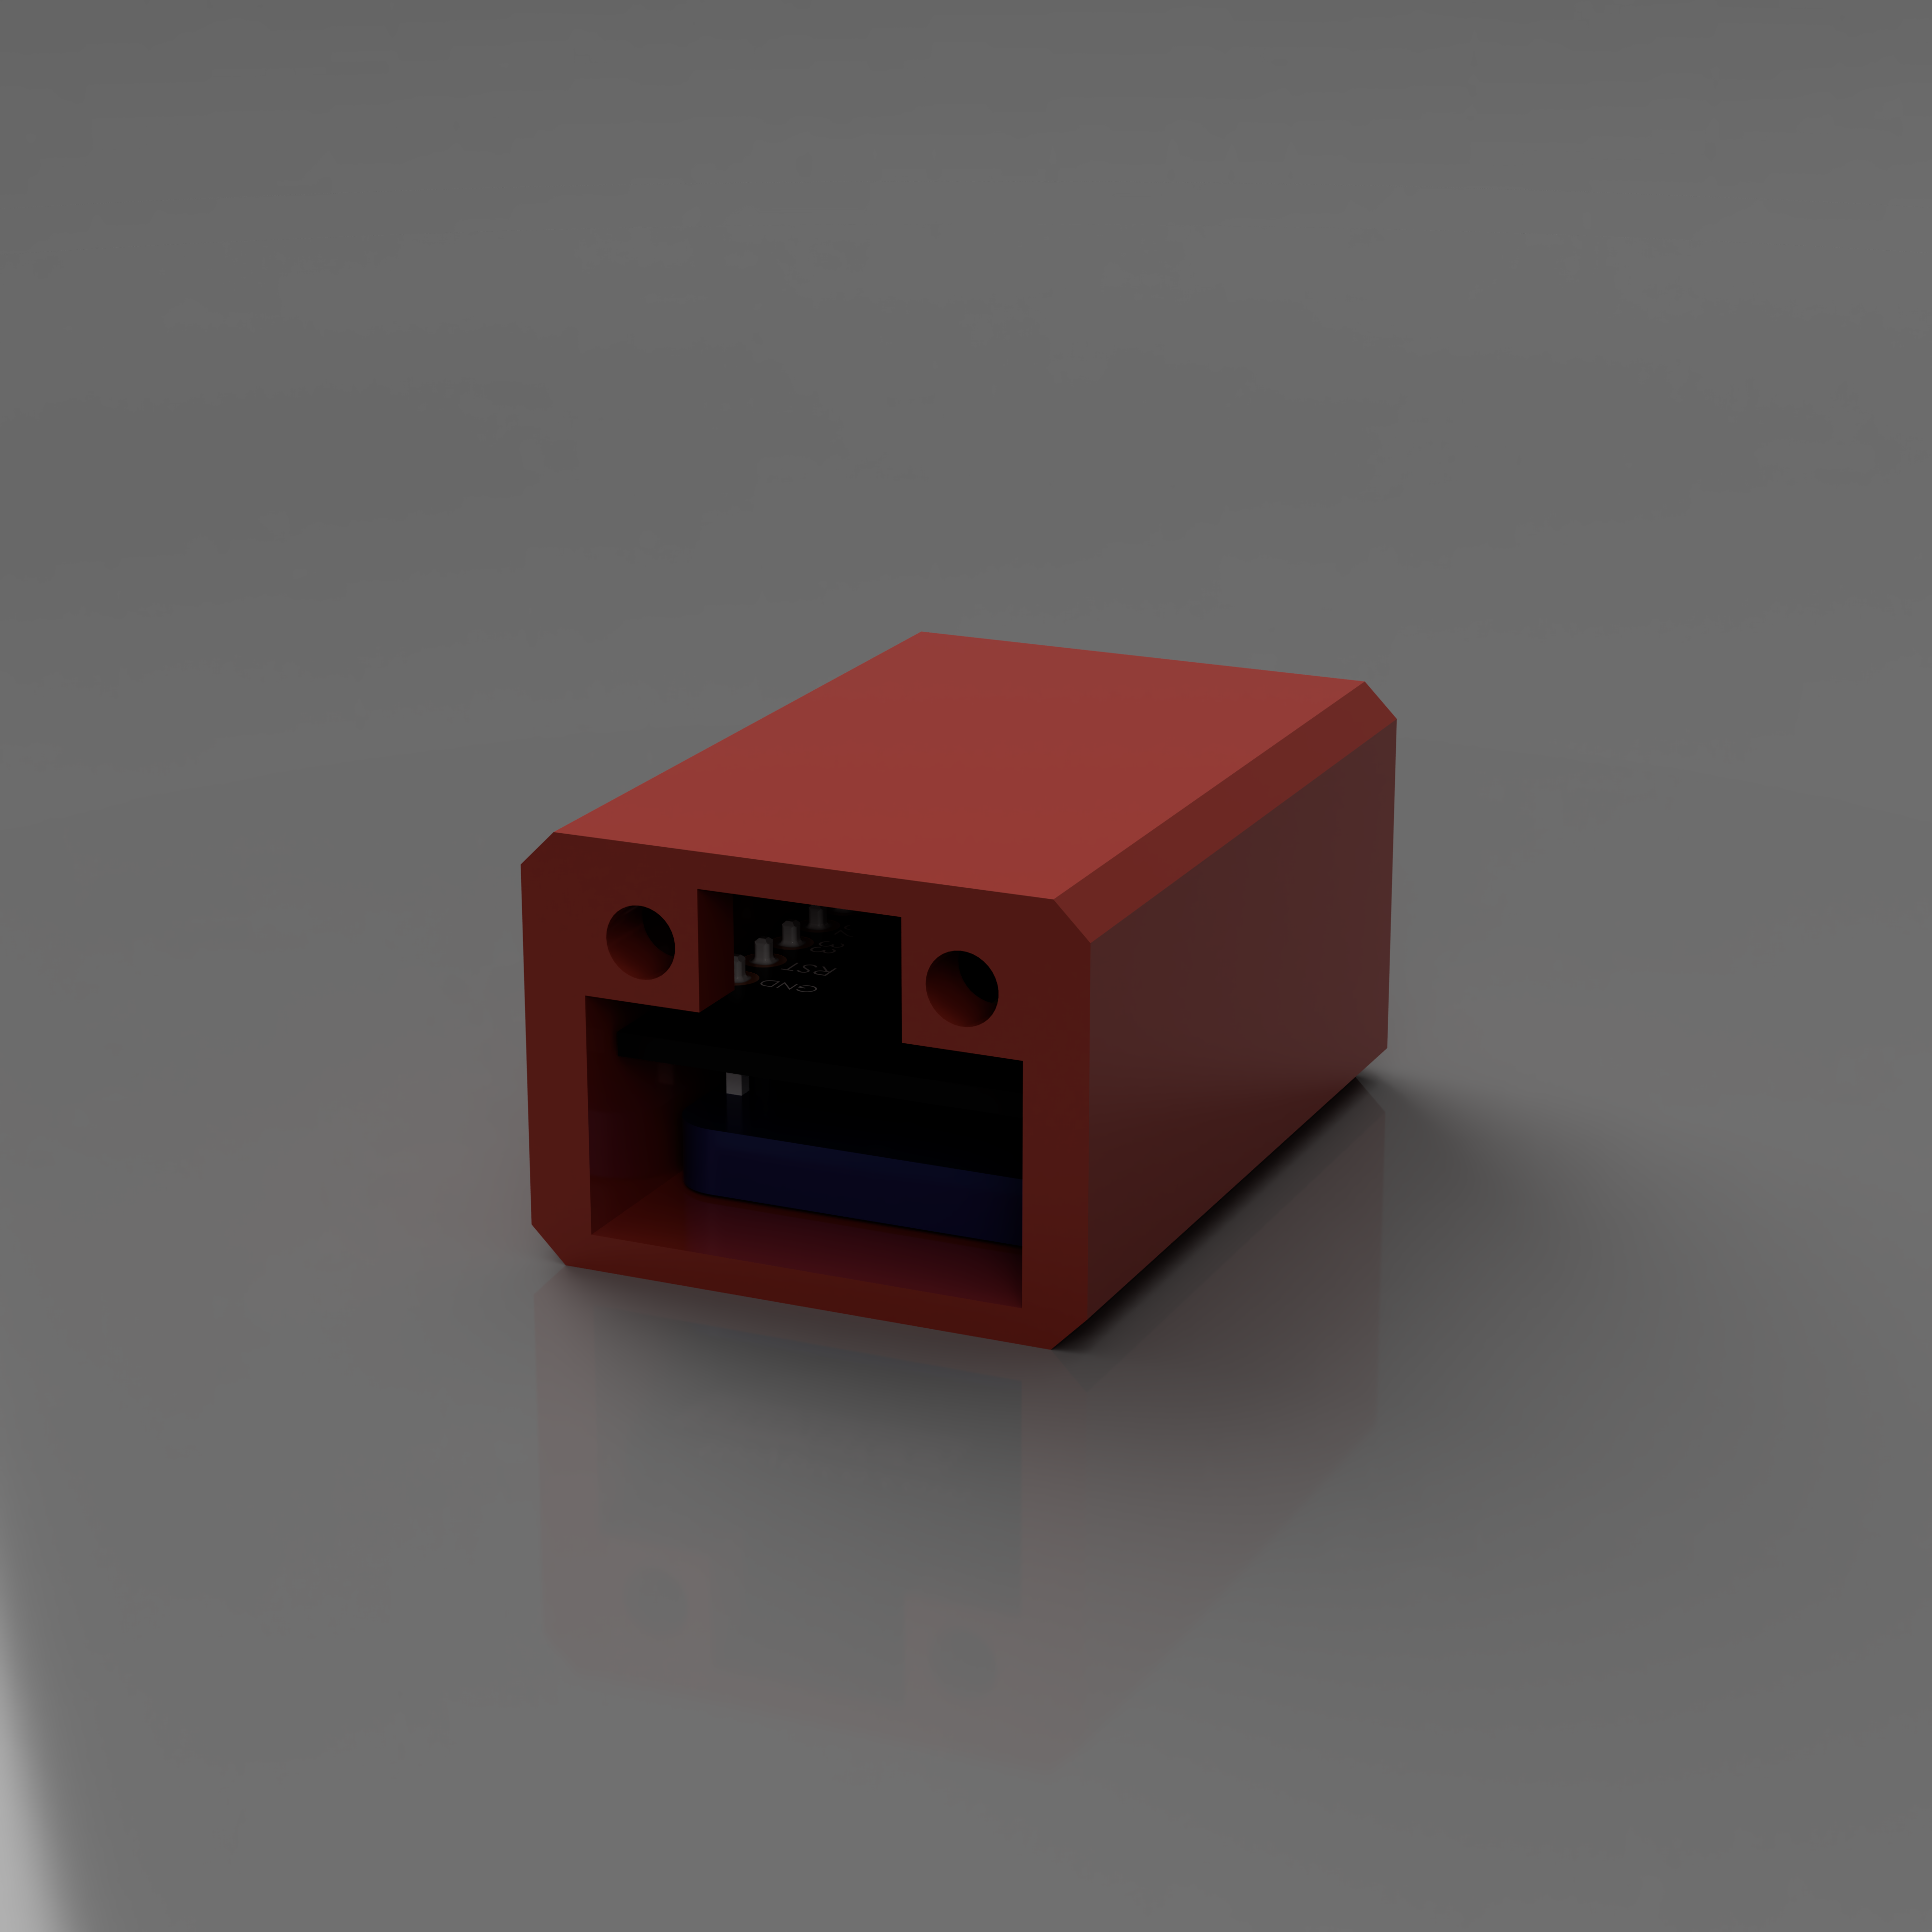
\includegraphics[width=.8\linewidth]{graphics/cad/wearable_2.png}
  \captionsetup{width=0.8\linewidth, justification=centering}
  \centering
  \captionof{figure}{Assembled wearable device}
  \label{fig:wearable_2}
\end{minipage}%
\begin{minipage}{.5\textwidth}
  \centering
  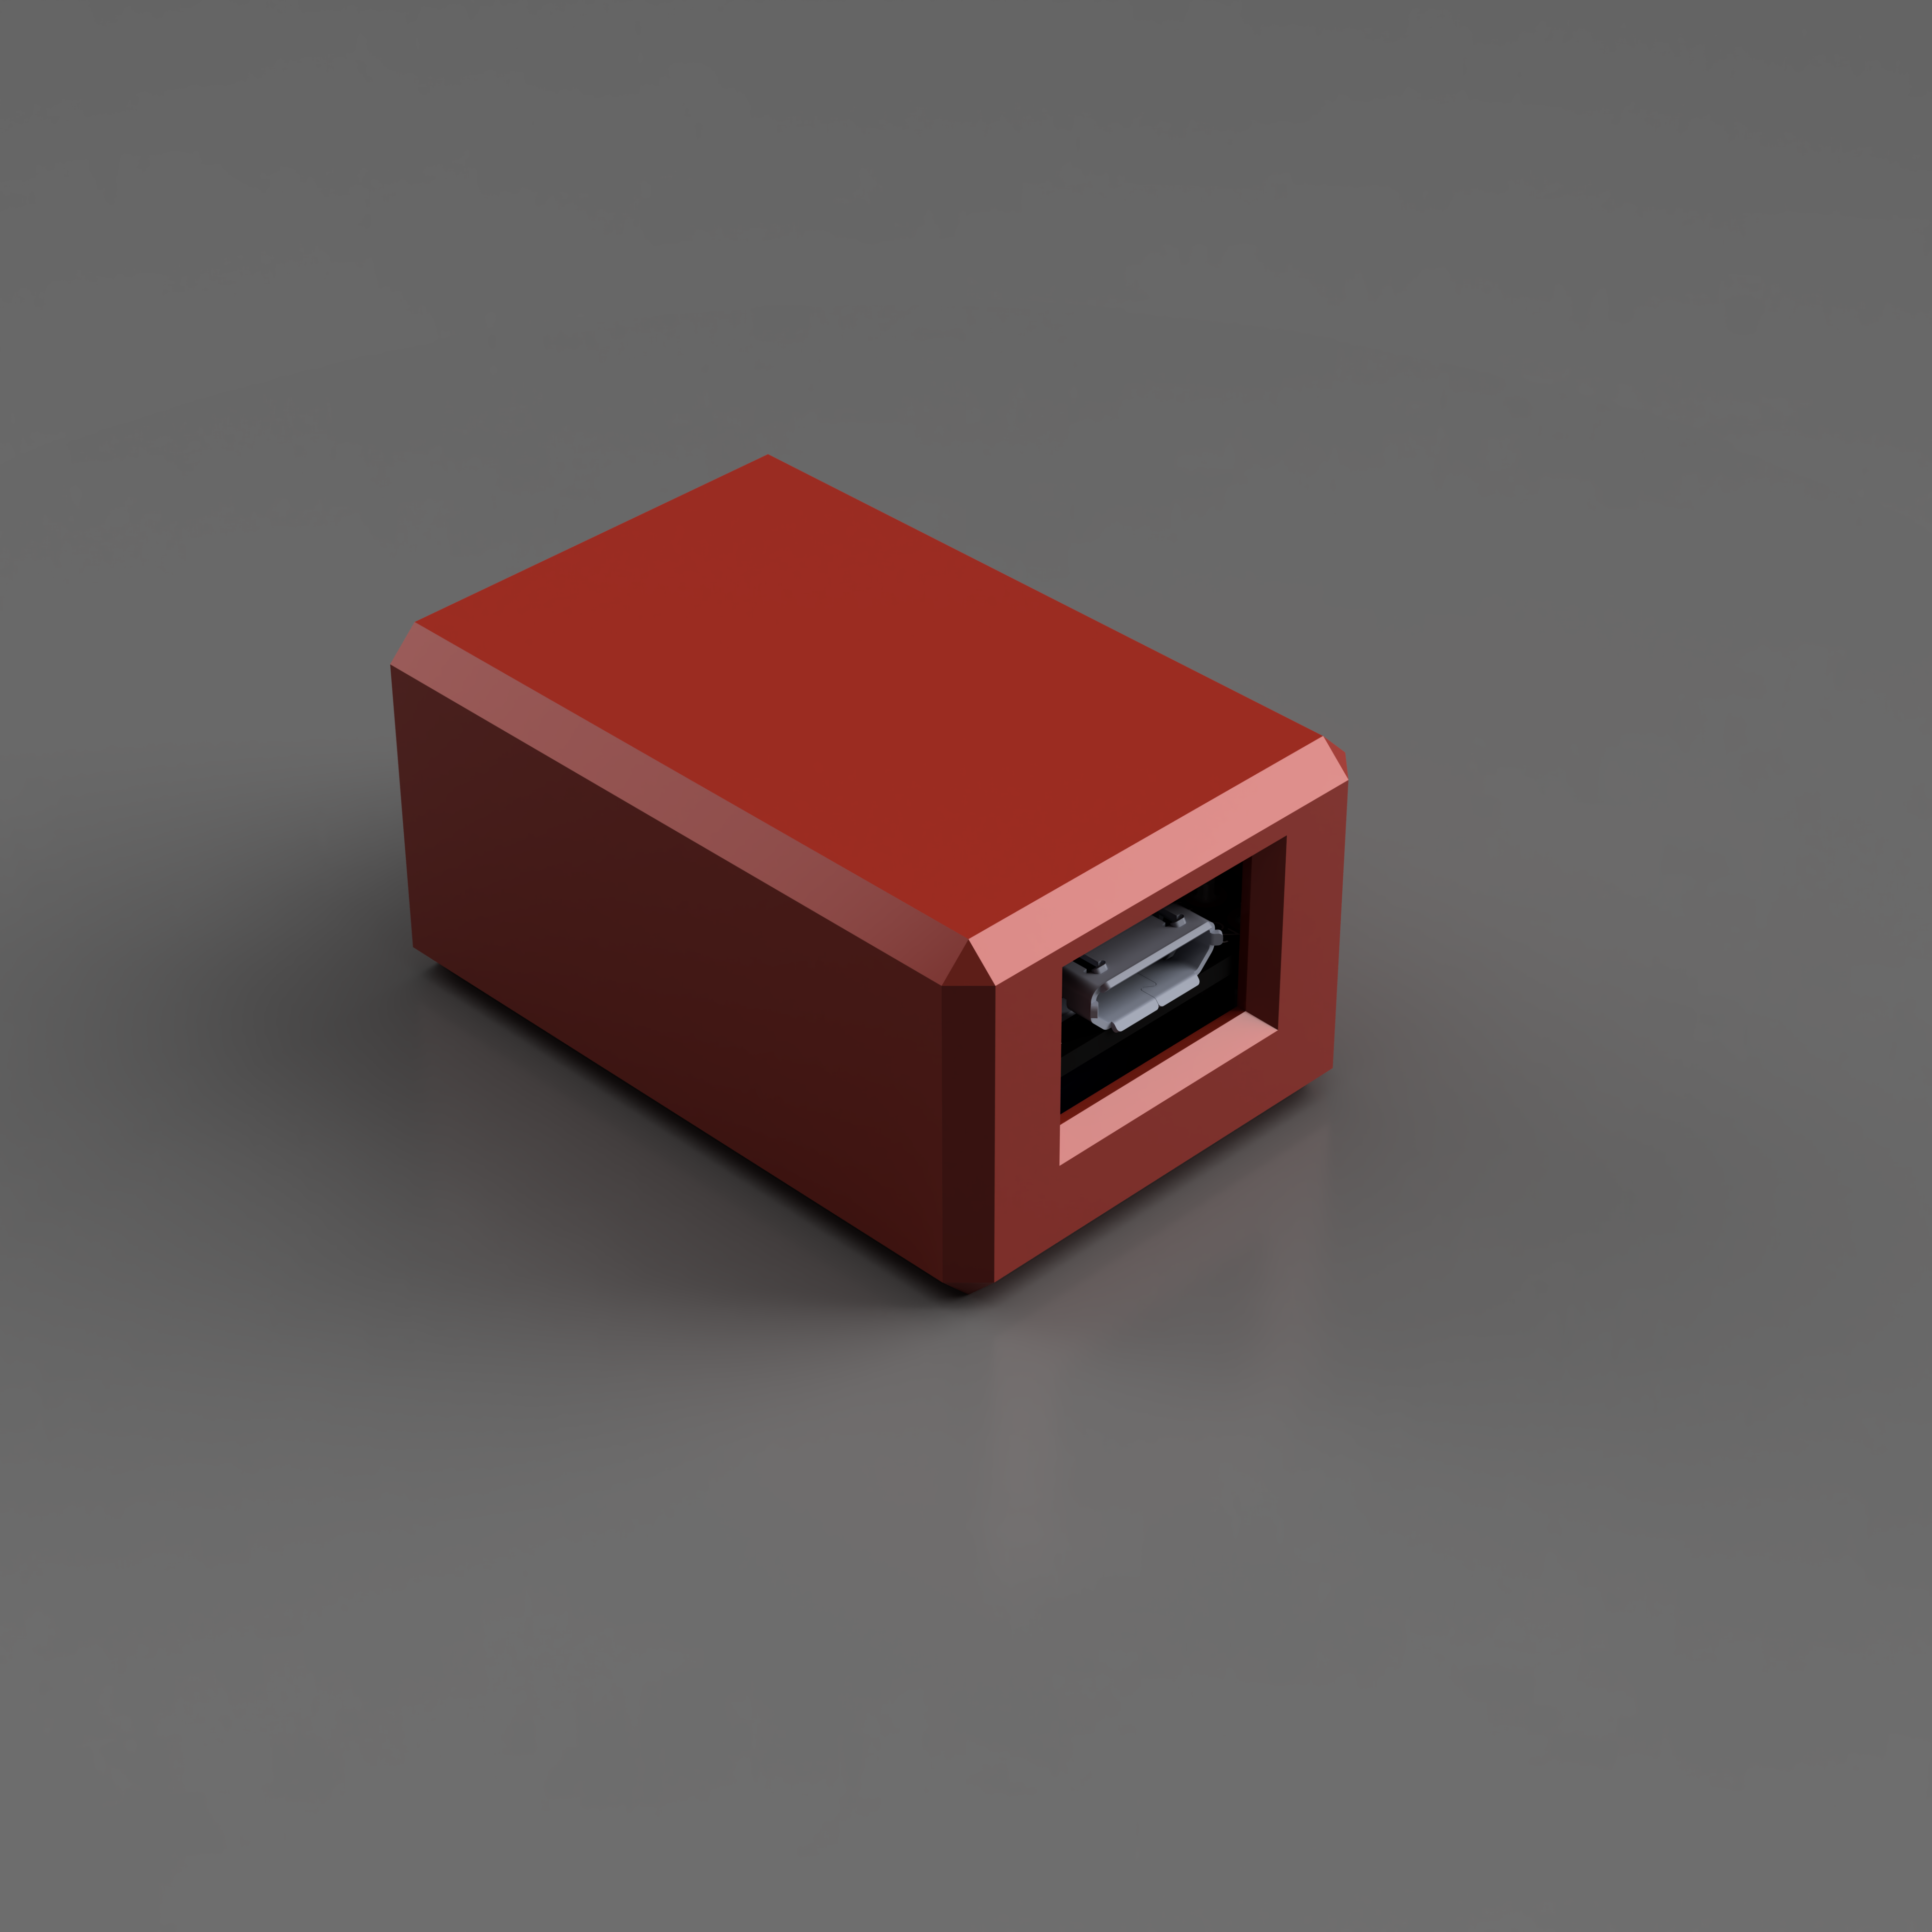
\includegraphics[width=.8\linewidth]{graphics/cad/wearable_1.png}
  \captionsetup{width=0.8\linewidth, justification=centering}
  \centering
  \captionof{figure}{Assembled wearable device}
  \label{fig:wearable_1}
\end{minipage}
\end{figure}

            We have designed and printed two different mounting options to begin with, the first being a "clip on" style attachment, that allows the wearable device to be clipped into pockets, clothing, or existing bands or straps the user may be wearing. This was designed to be a tight, friction fit between the casing and the clip, to ensure there is less chance of the item becoming loose over time.

            \begin{figure}[H]
\centering
\begin{minipage}{.5\textwidth}
  \centering
  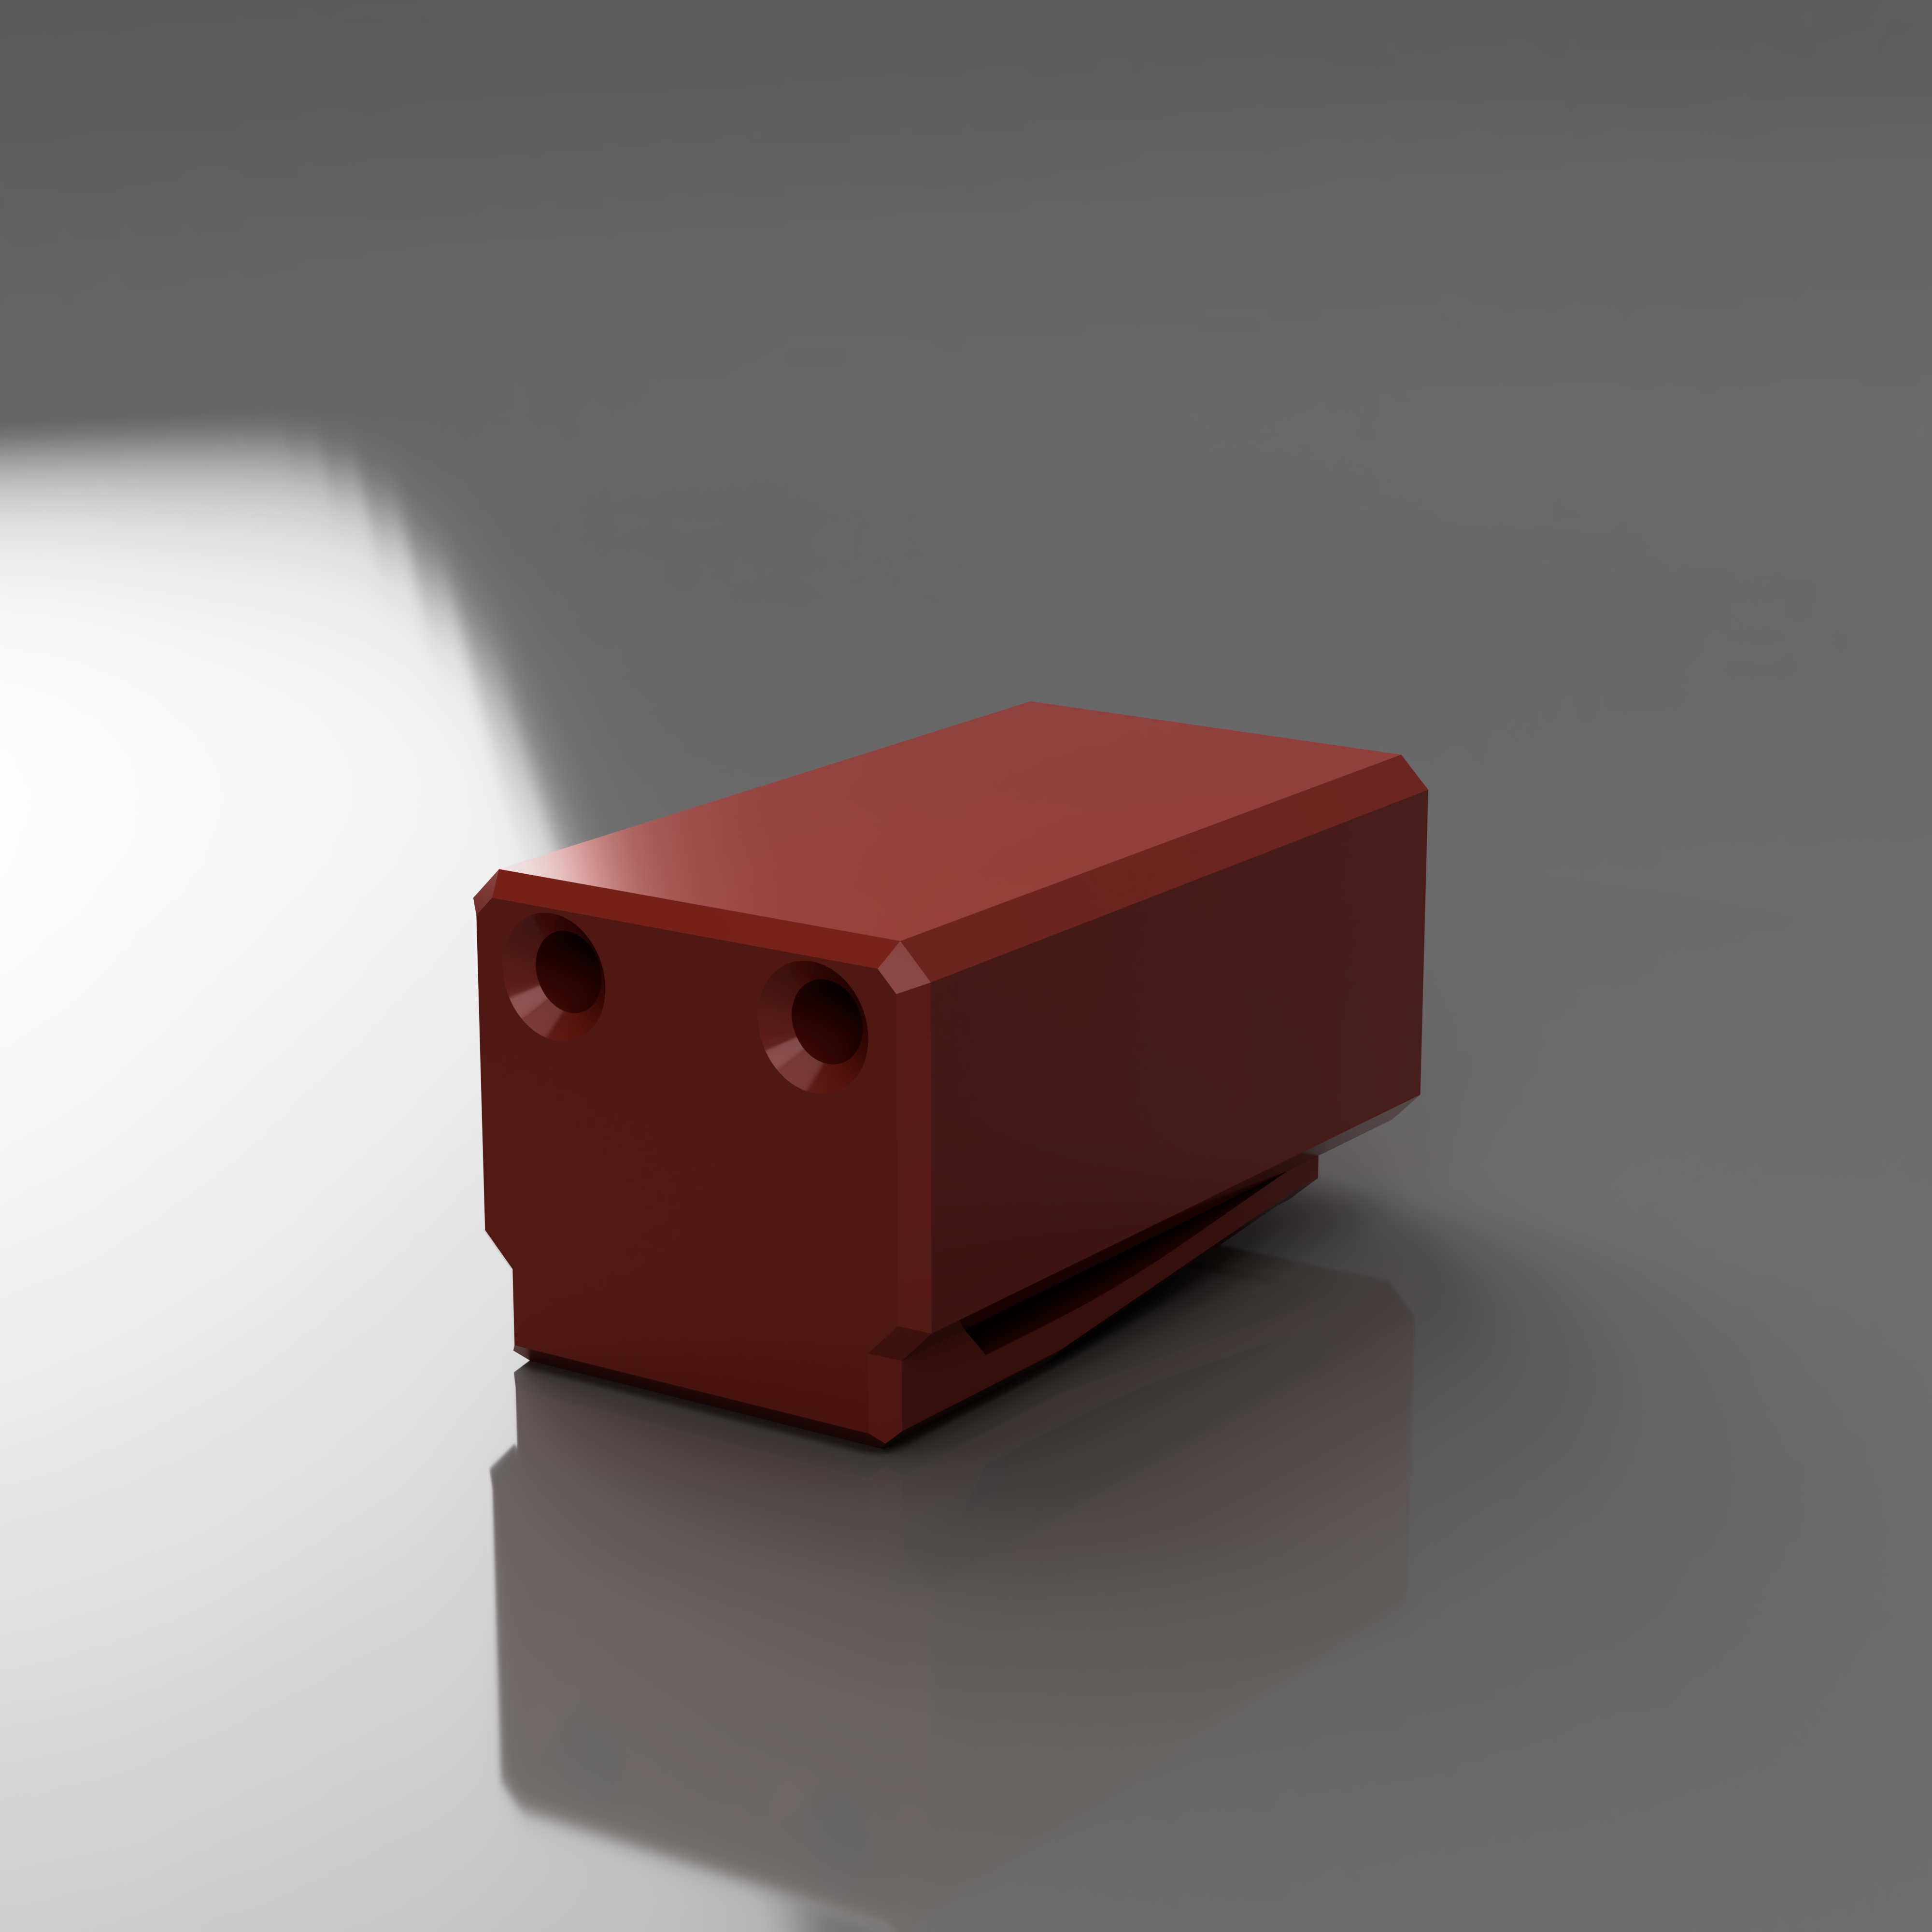
\includegraphics[width=.8\linewidth]{graphics/cad/wearable_clip_1.png}
  \captionsetup{width=0.8\linewidth, justification=centering}
  \centering
  \captionof{figure}{Wearable device with clip attachment}
  \label{fig:wearable_clip_1}
\end{minipage}%
\begin{minipage}{.5\textwidth}
  \centering
  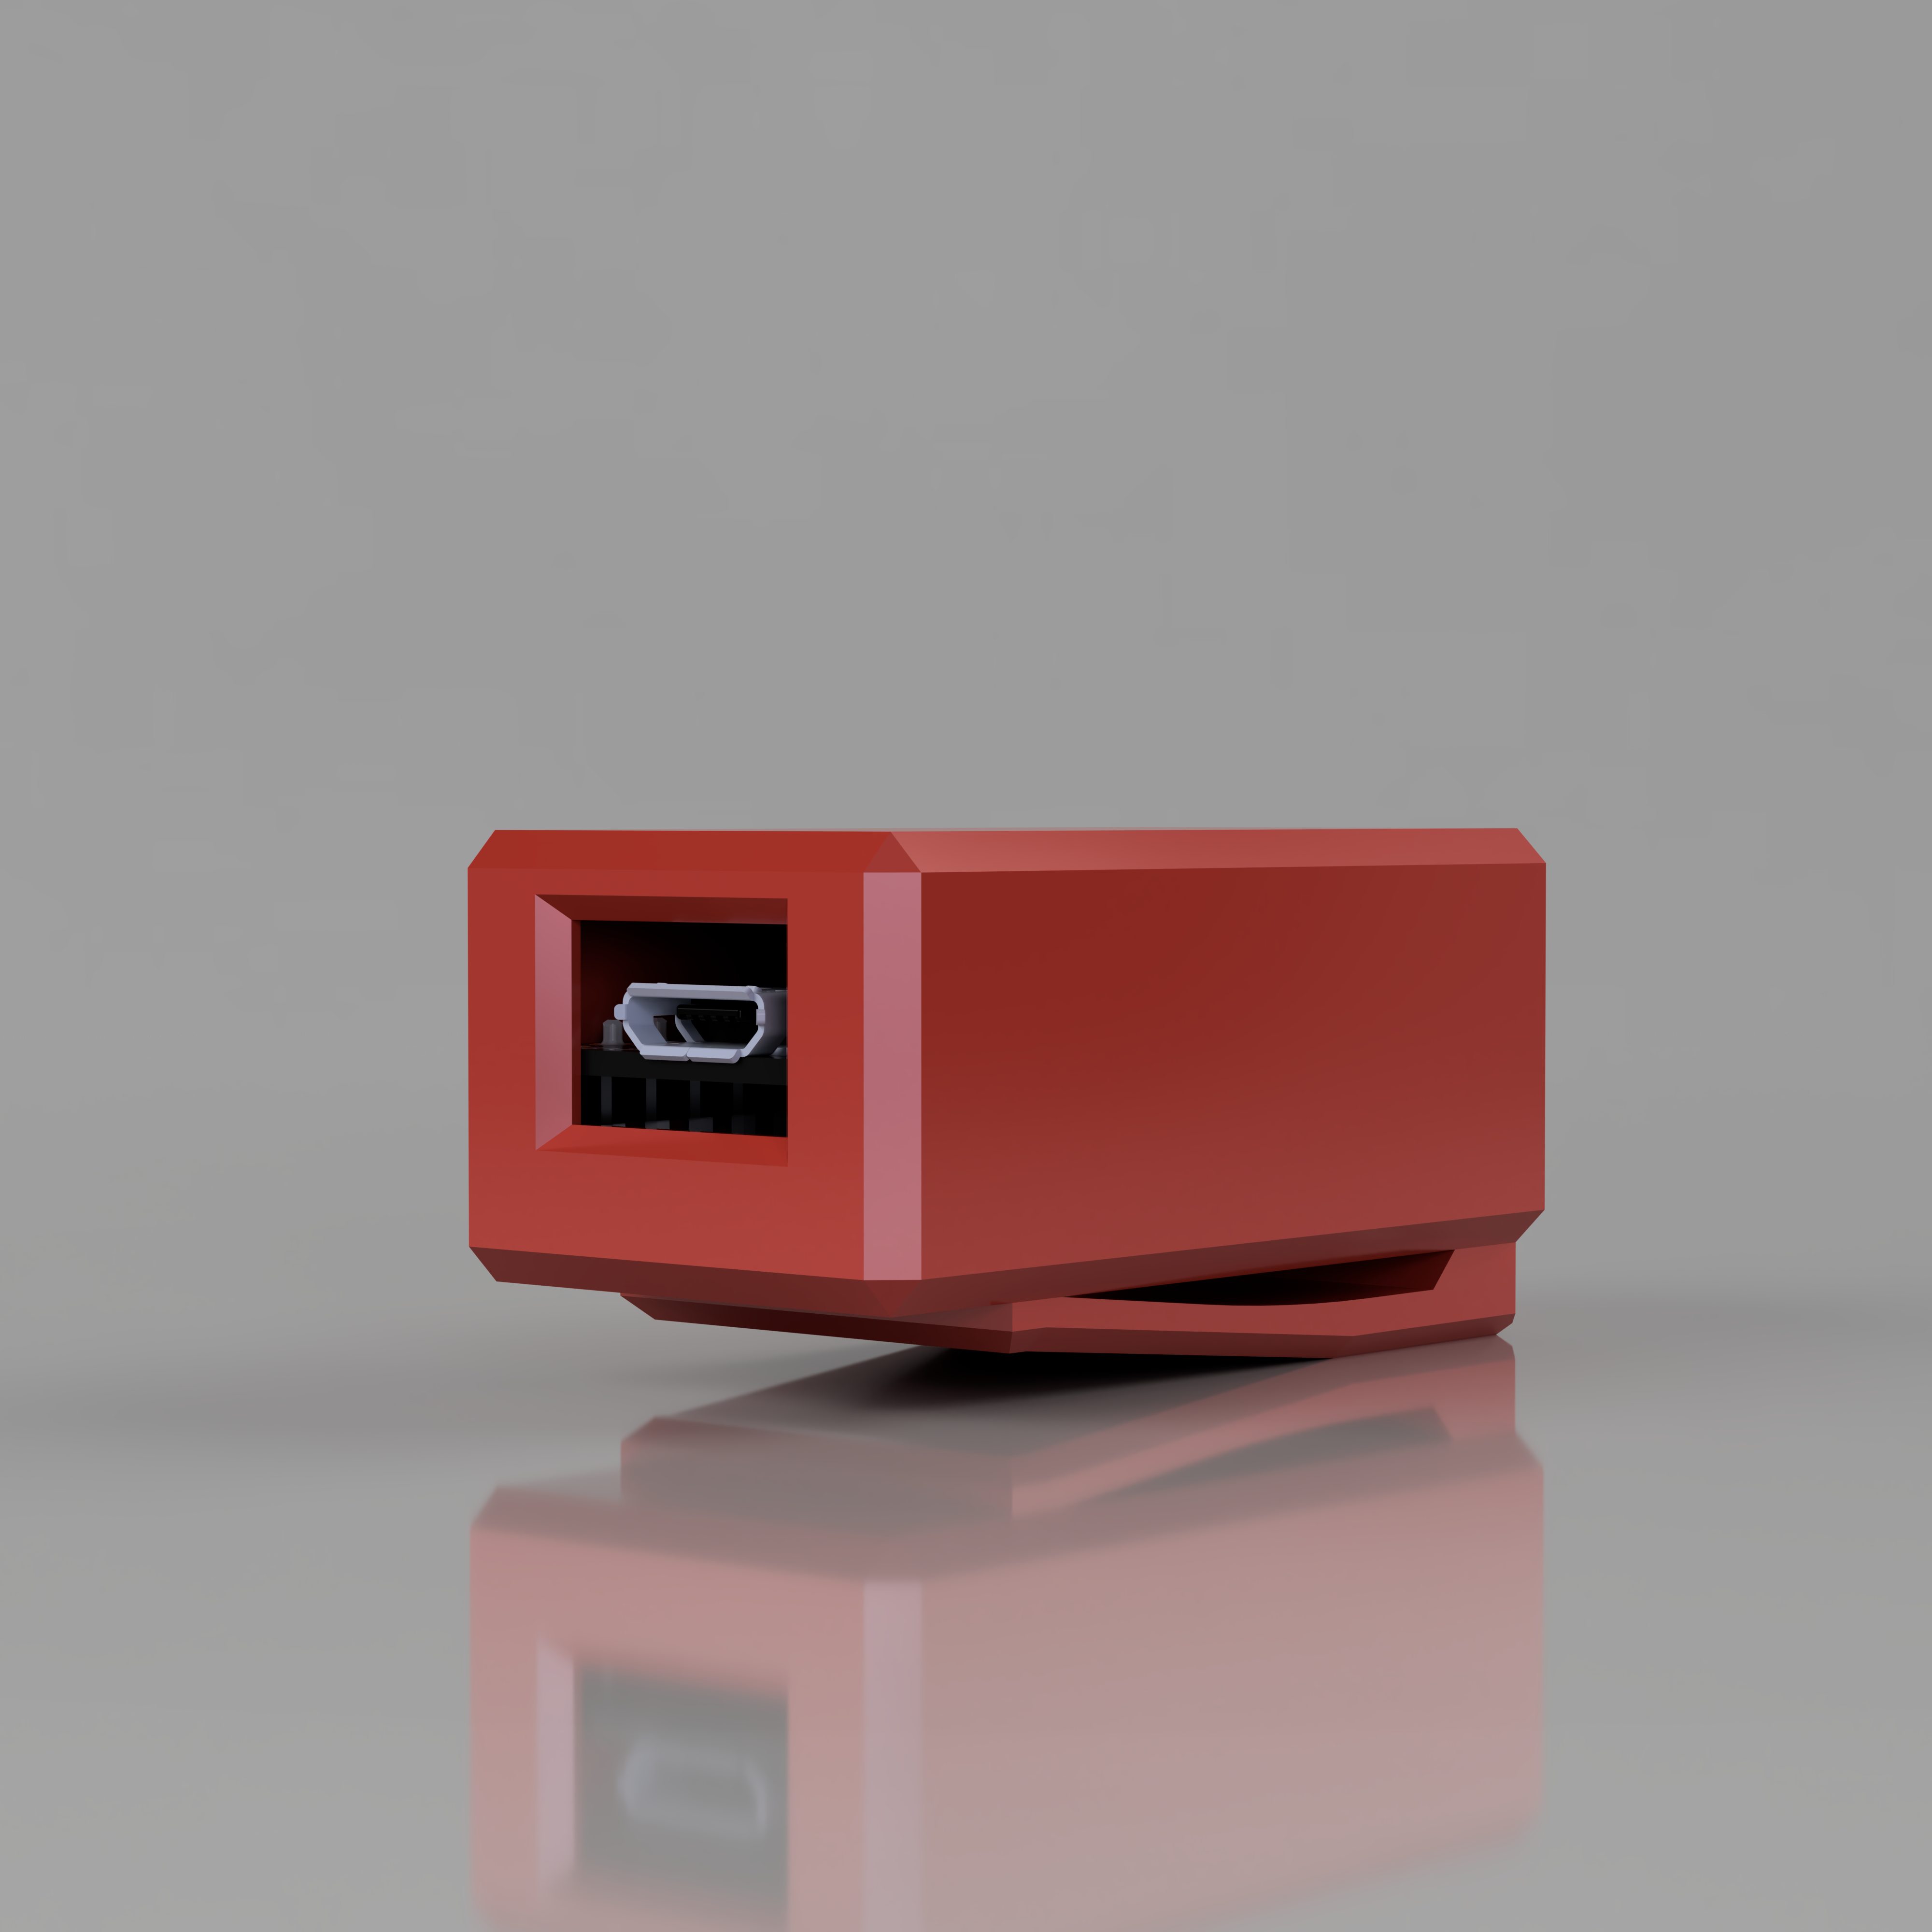
\includegraphics[width=.8\linewidth]{graphics/cad/wearable_clip_2.png}
  \captionsetup{width=0.8\linewidth, justification=centering}
  \centering
  \captionof{figure}{Wearable device with clip attachment}
  \label{fig:wearable_clip_2}
\end{minipage}
\end{figure}

            The second attachment option is a watch strap mount. This allows the wearable device to be used with any standard 22mm watchstrap, and the idea behind this is to allow for a more comfortable, and familiar feel on the arm. Patients aren't always happy trying new things due to their condition, but this should allow for existing watch straps to be used, and making them feel at home with their new device.

            \begin{figure}[H]
\centering
\begin{minipage}{.5\textwidth}
  \centering
  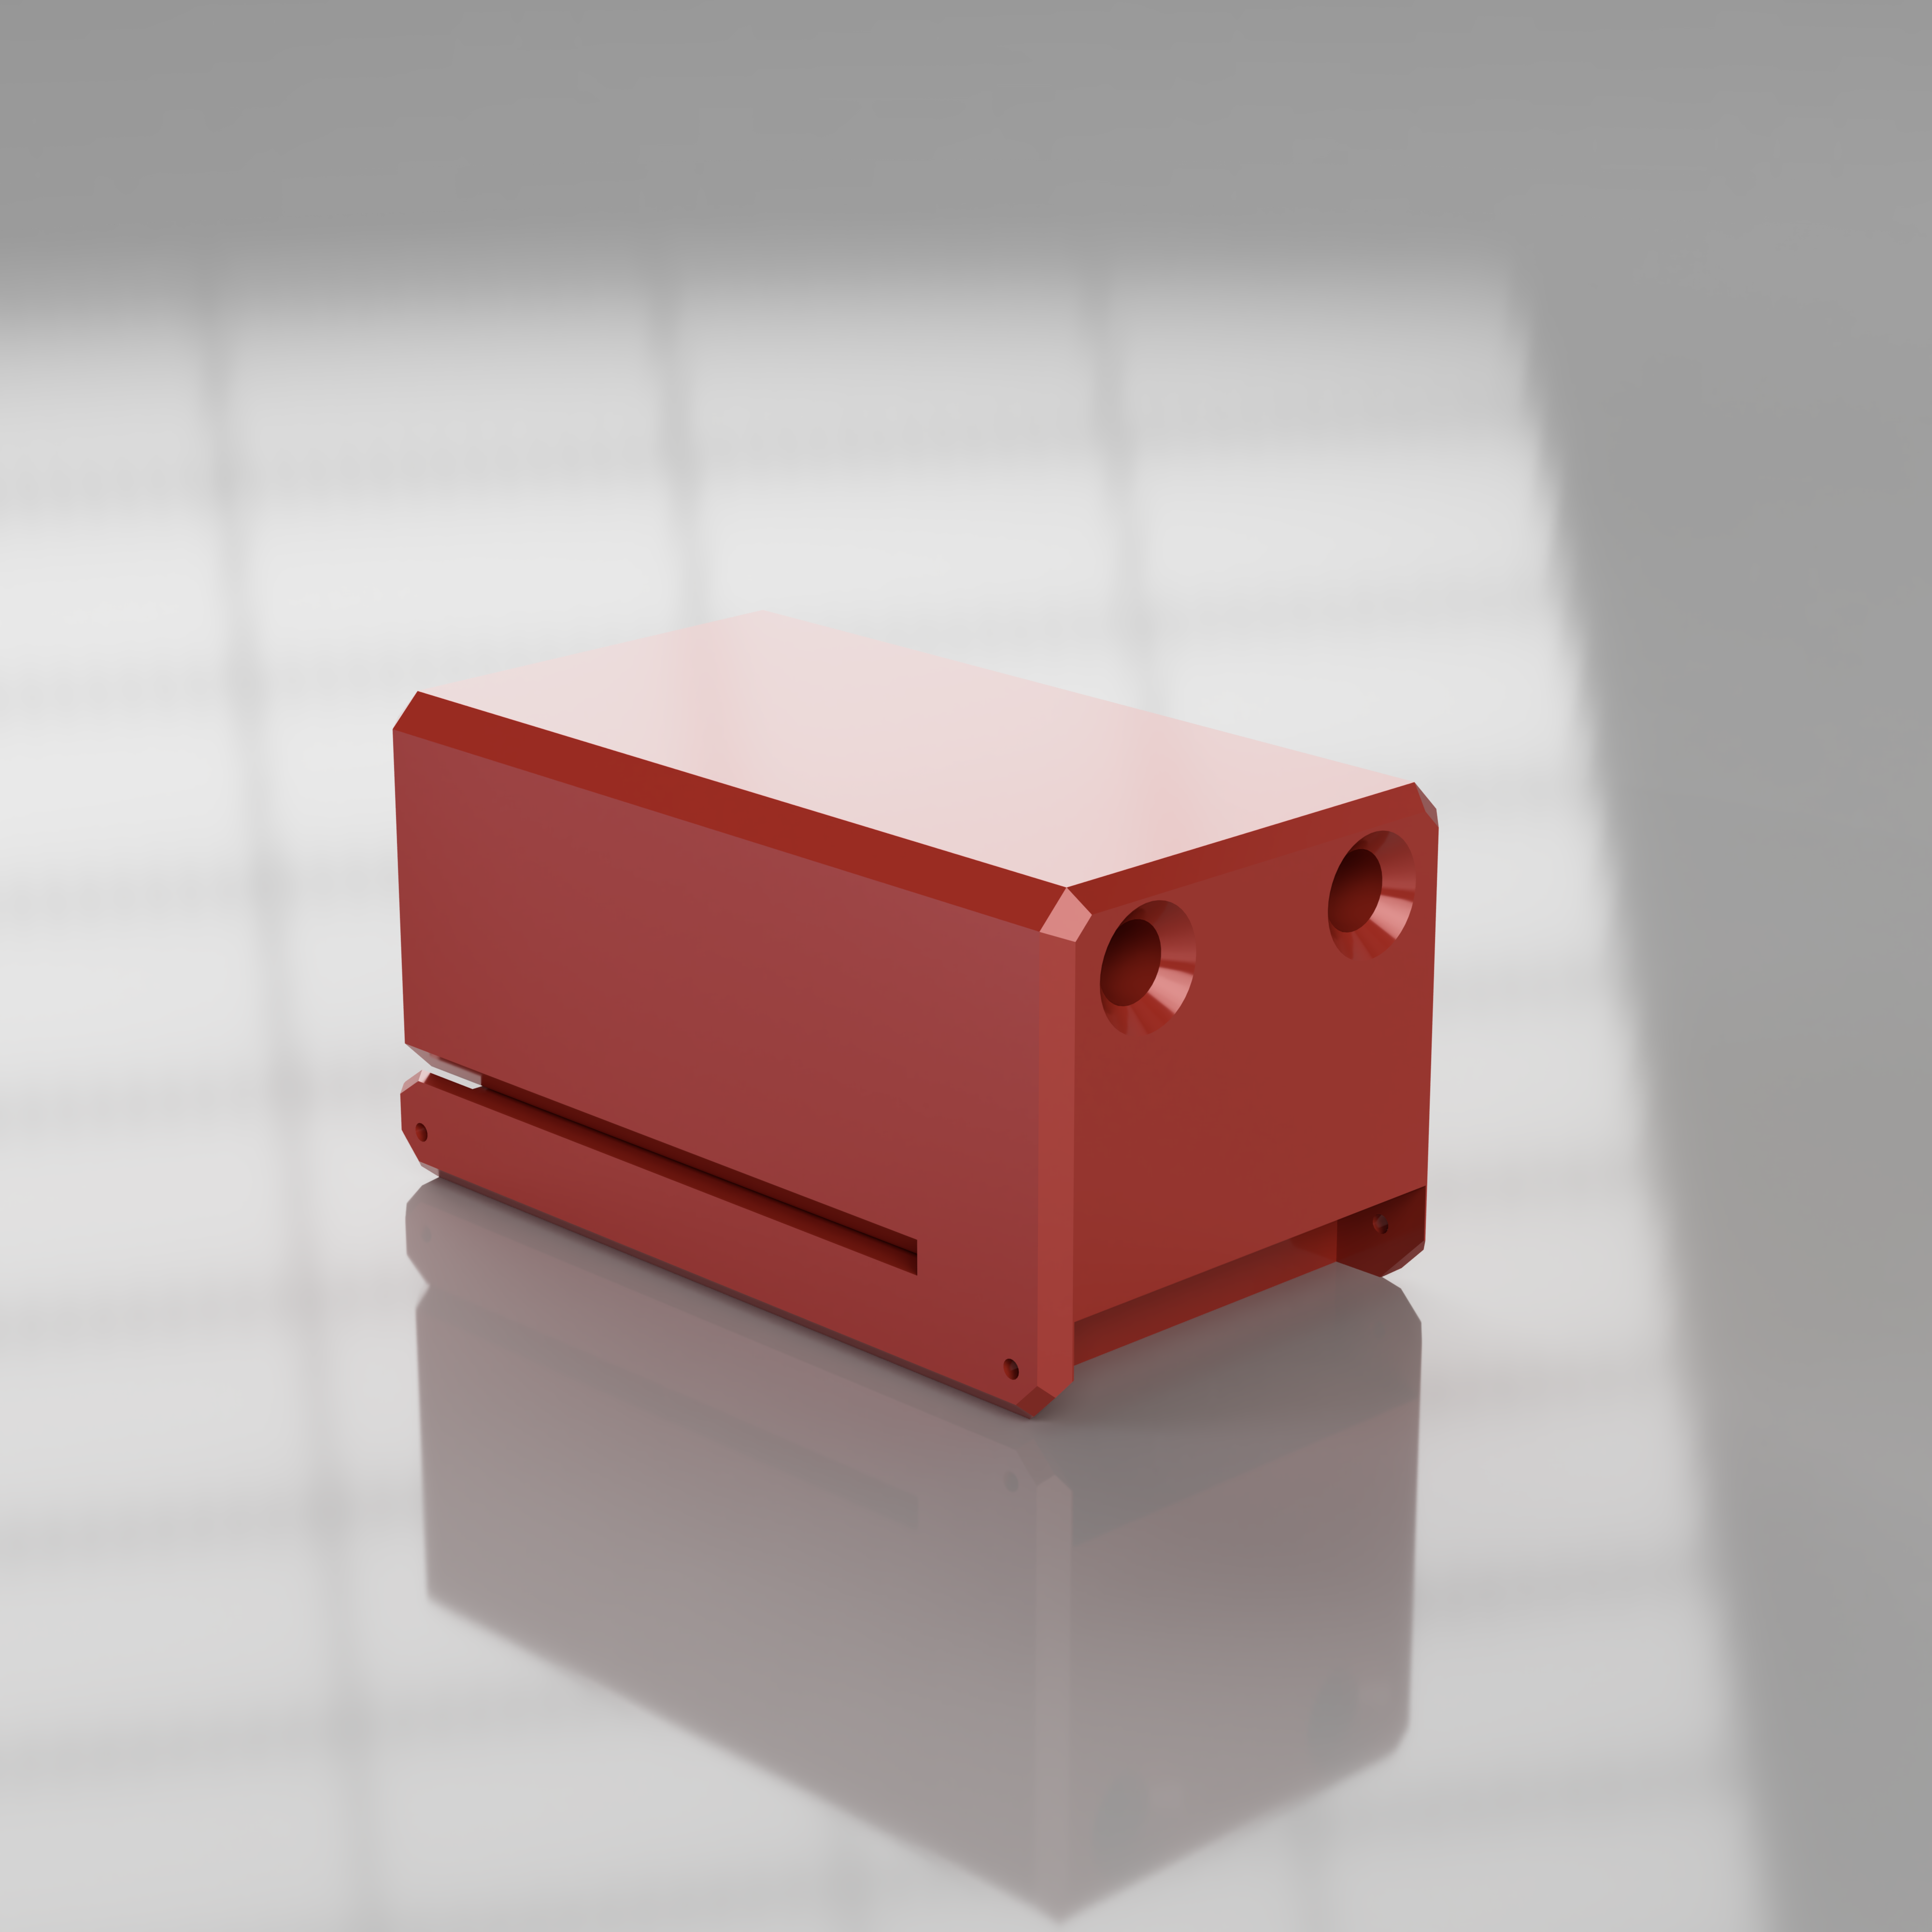
\includegraphics[width=.8\linewidth]{graphics/cad/wearable_strap_1.png}
  \captionsetup{width=0.8\linewidth, justification=centering}
  \centering
  \captionof{figure}{Wearable device with strap attachment}
  \label{fig:wearable_strap_1}
\end{minipage}%
\begin{minipage}{.5\textwidth}
  \centering
  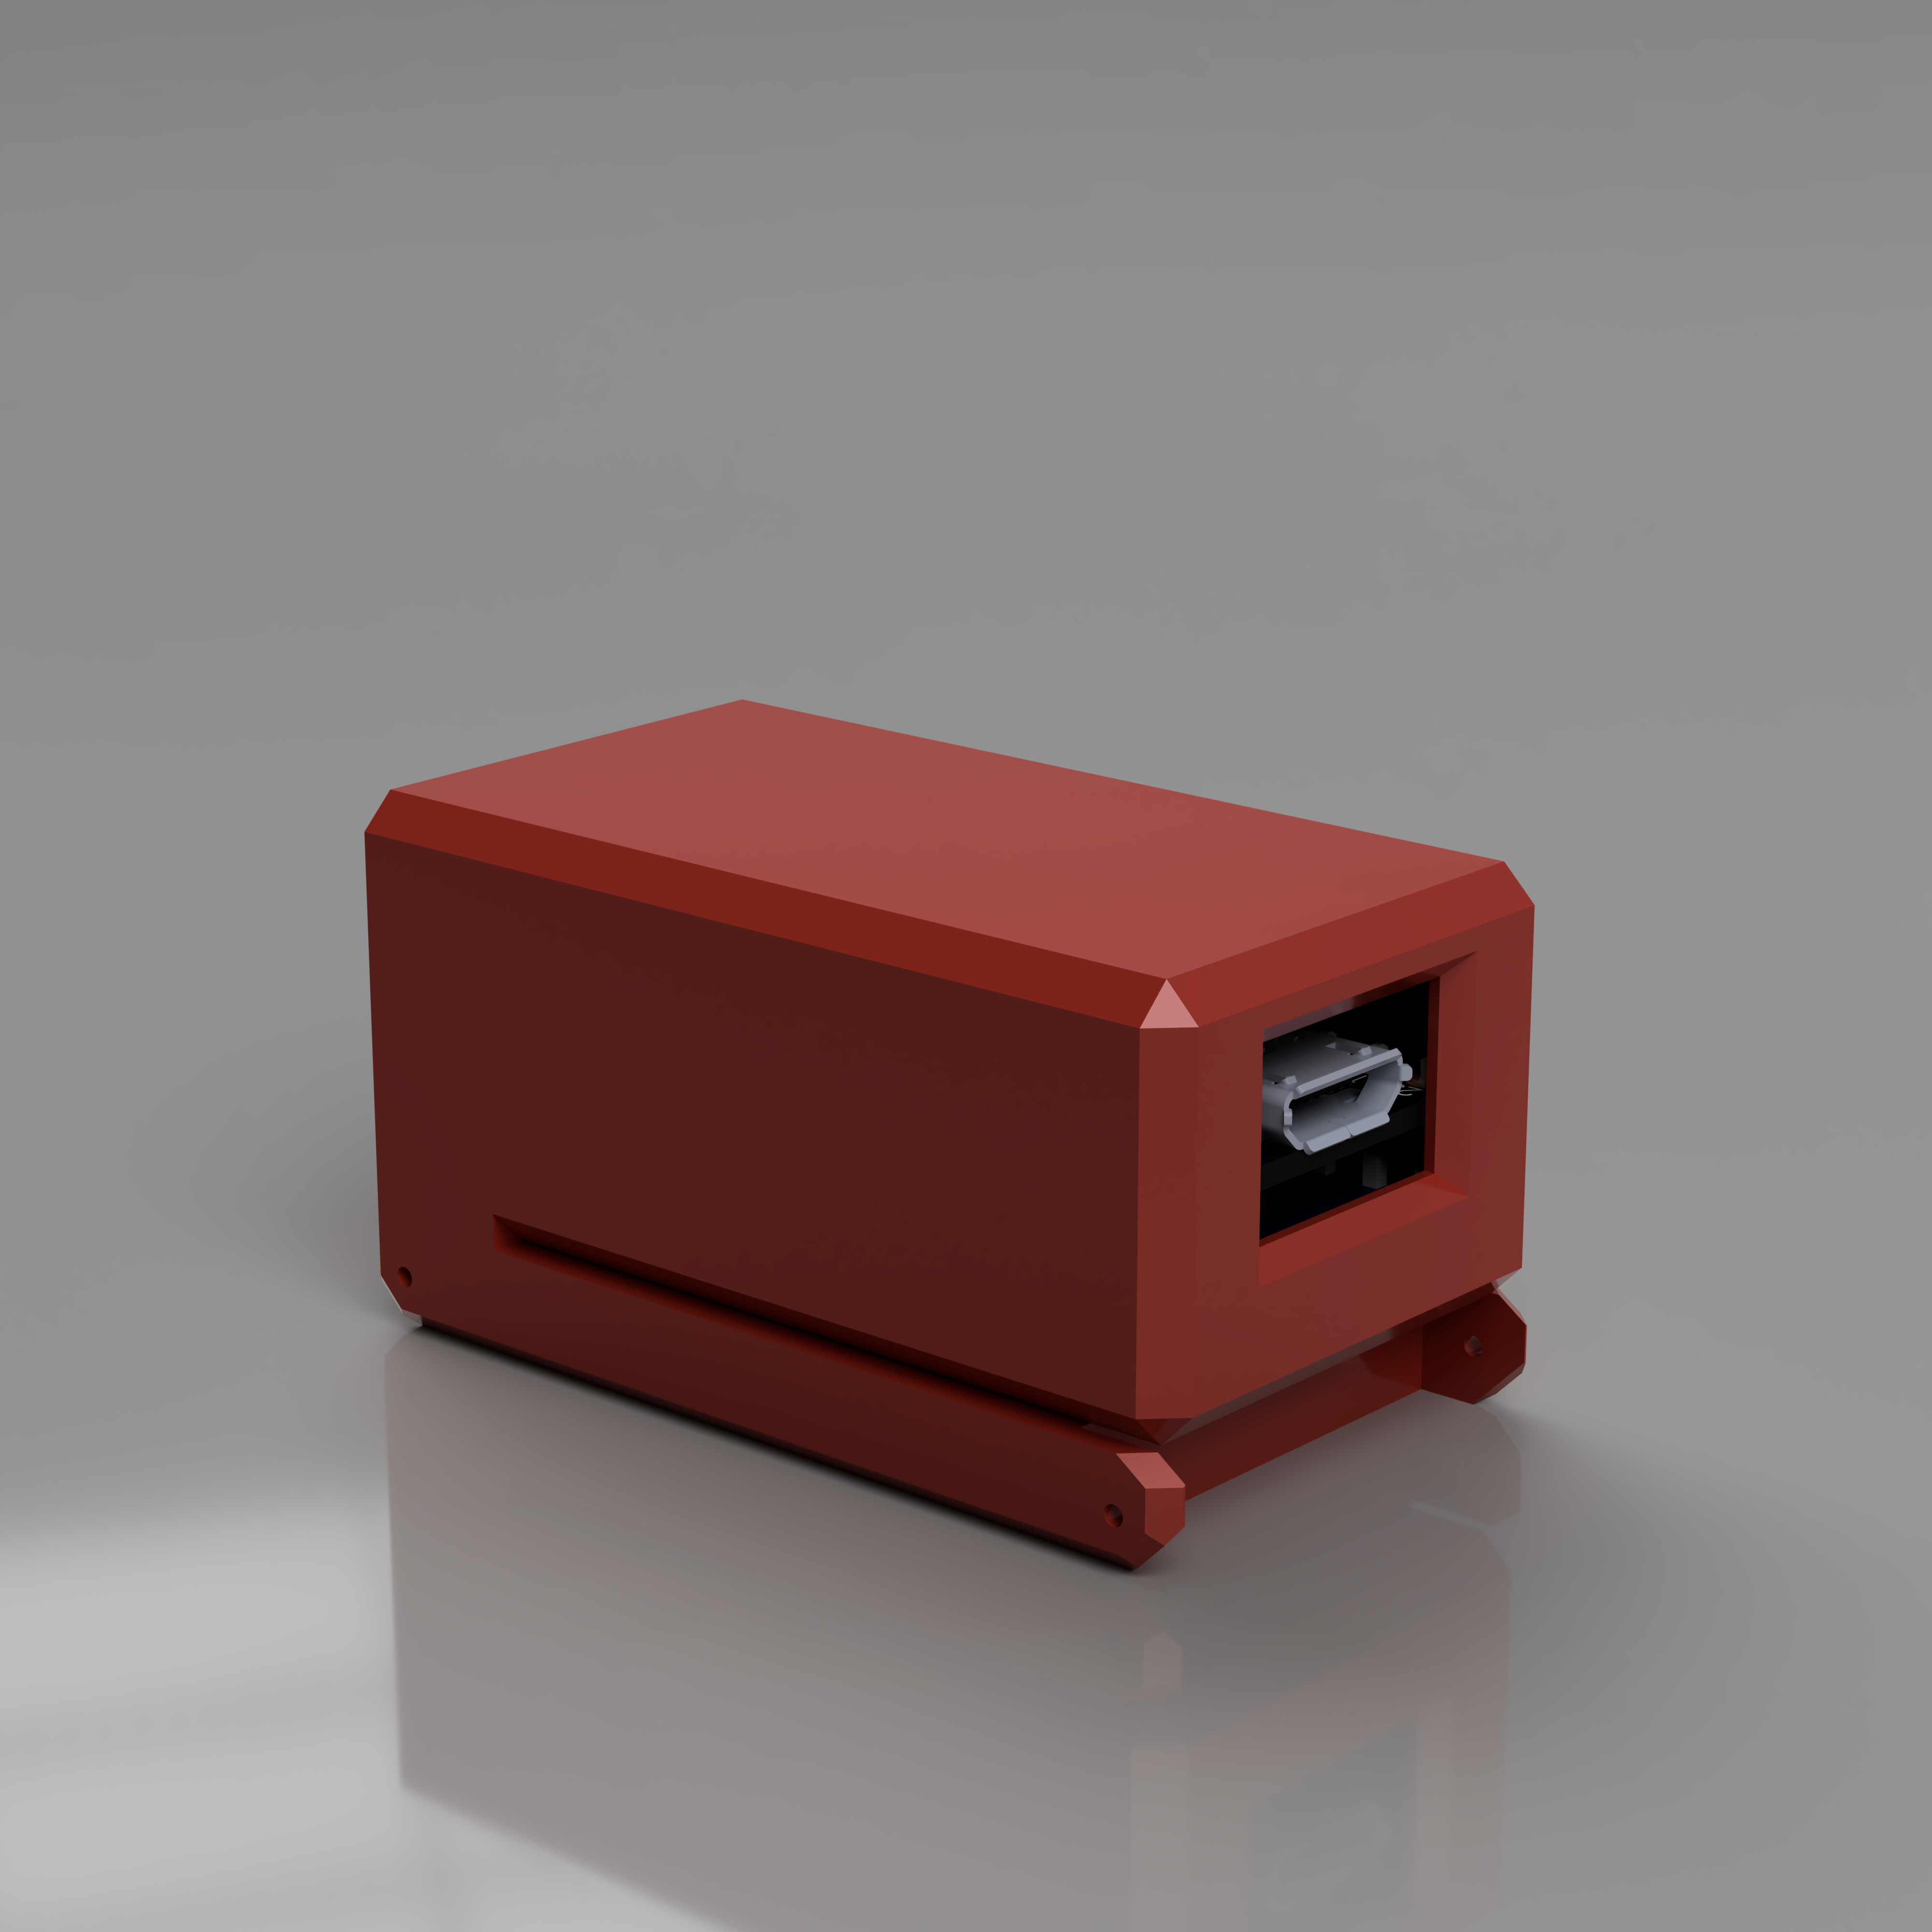
\includegraphics[width=.8\linewidth]{graphics/cad/wearable_strap_2.png}
  \captionsetup{width=0.8\linewidth, justification=centering}
  \centering
  \captionof{figure}{Wearable device with strap attachment}
  \label{fig:wearable_strap_2}
\end{minipage}
\end{figure}

        \subsection{Prototype}
        \label{subsec:Prototype_wearable}

            The prototype was assembled using M3x8 stainless steel screws, which allowed for easy assembly and self tapping into the soft interior plastic, which was tolerances for this. In the future, it would be ideal to use heatset inserts, to ensure the longevity of the threading.

            \begin{figure}[H]
\centering
\begin{minipage}{.5\textwidth}
  \centering
  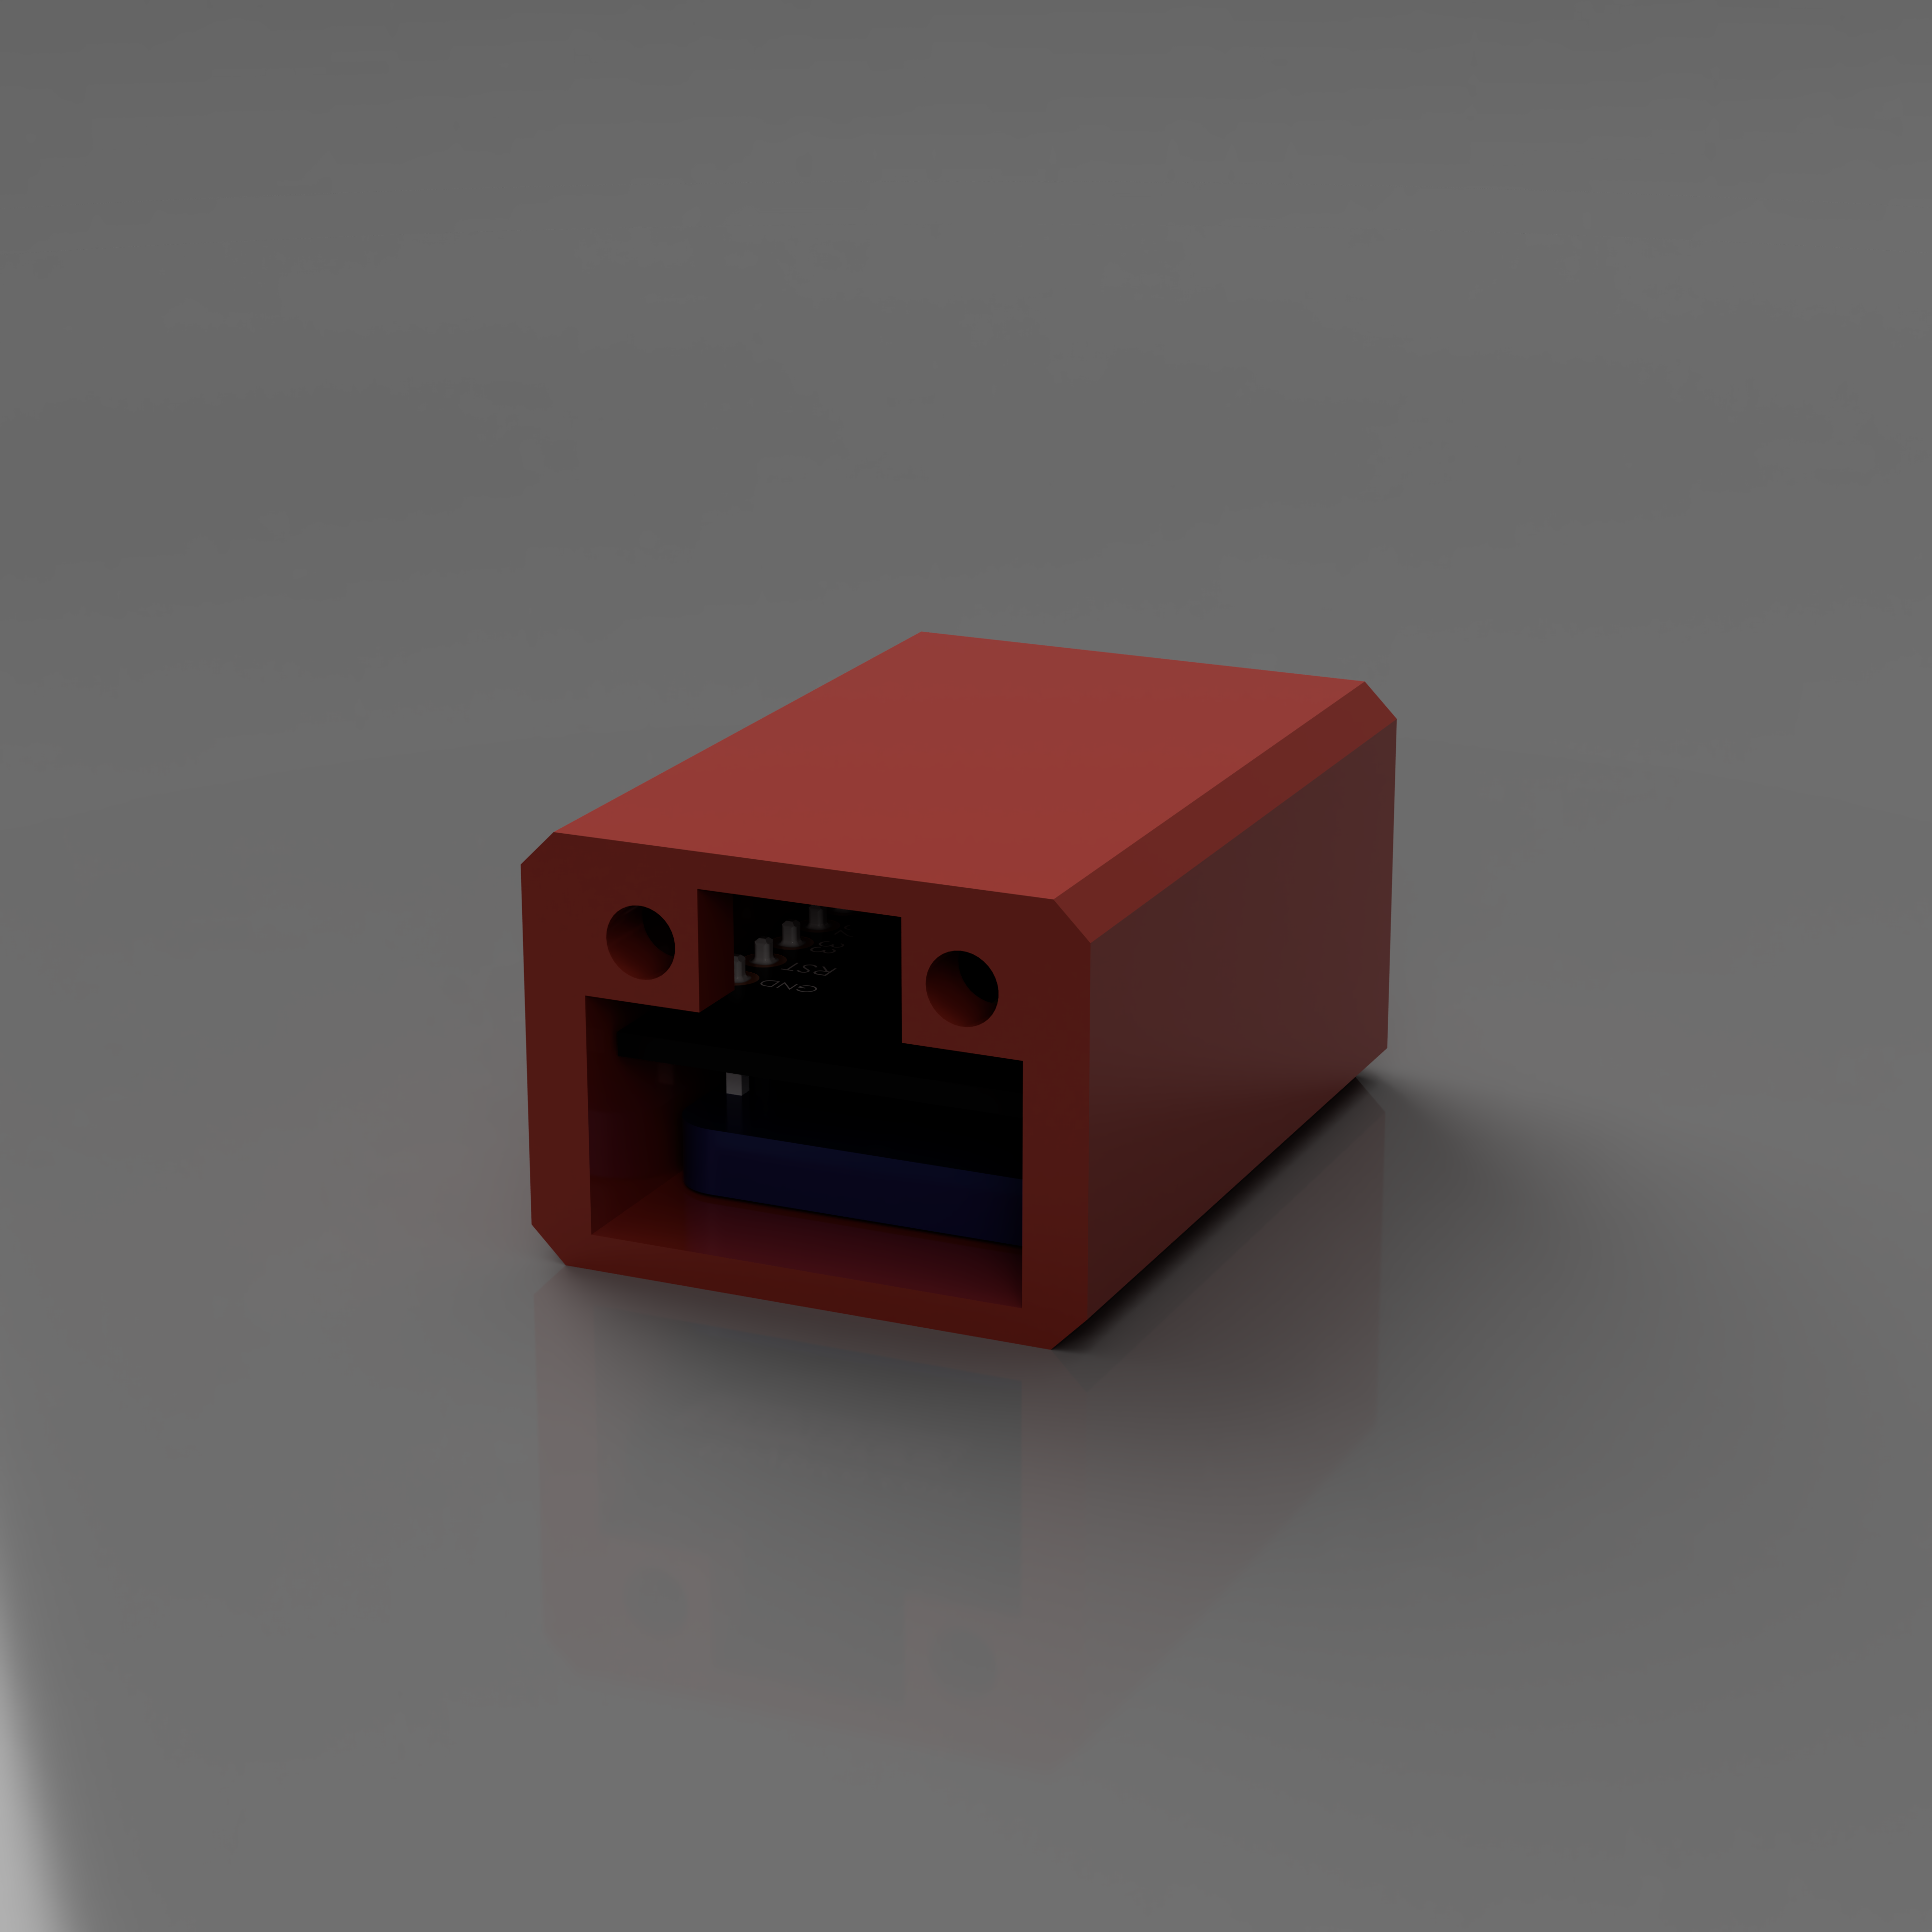
\includegraphics[width=.8\linewidth]{graphics/cad/wearable_2.png}
  \captionsetup{width=0.8\linewidth, justification=centering}
  \centering
  \captionof{figure}{Assembled wearable device}
  \label{fig:wearable_2}
\end{minipage}%
\begin{minipage}{.5\textwidth}
  \centering
  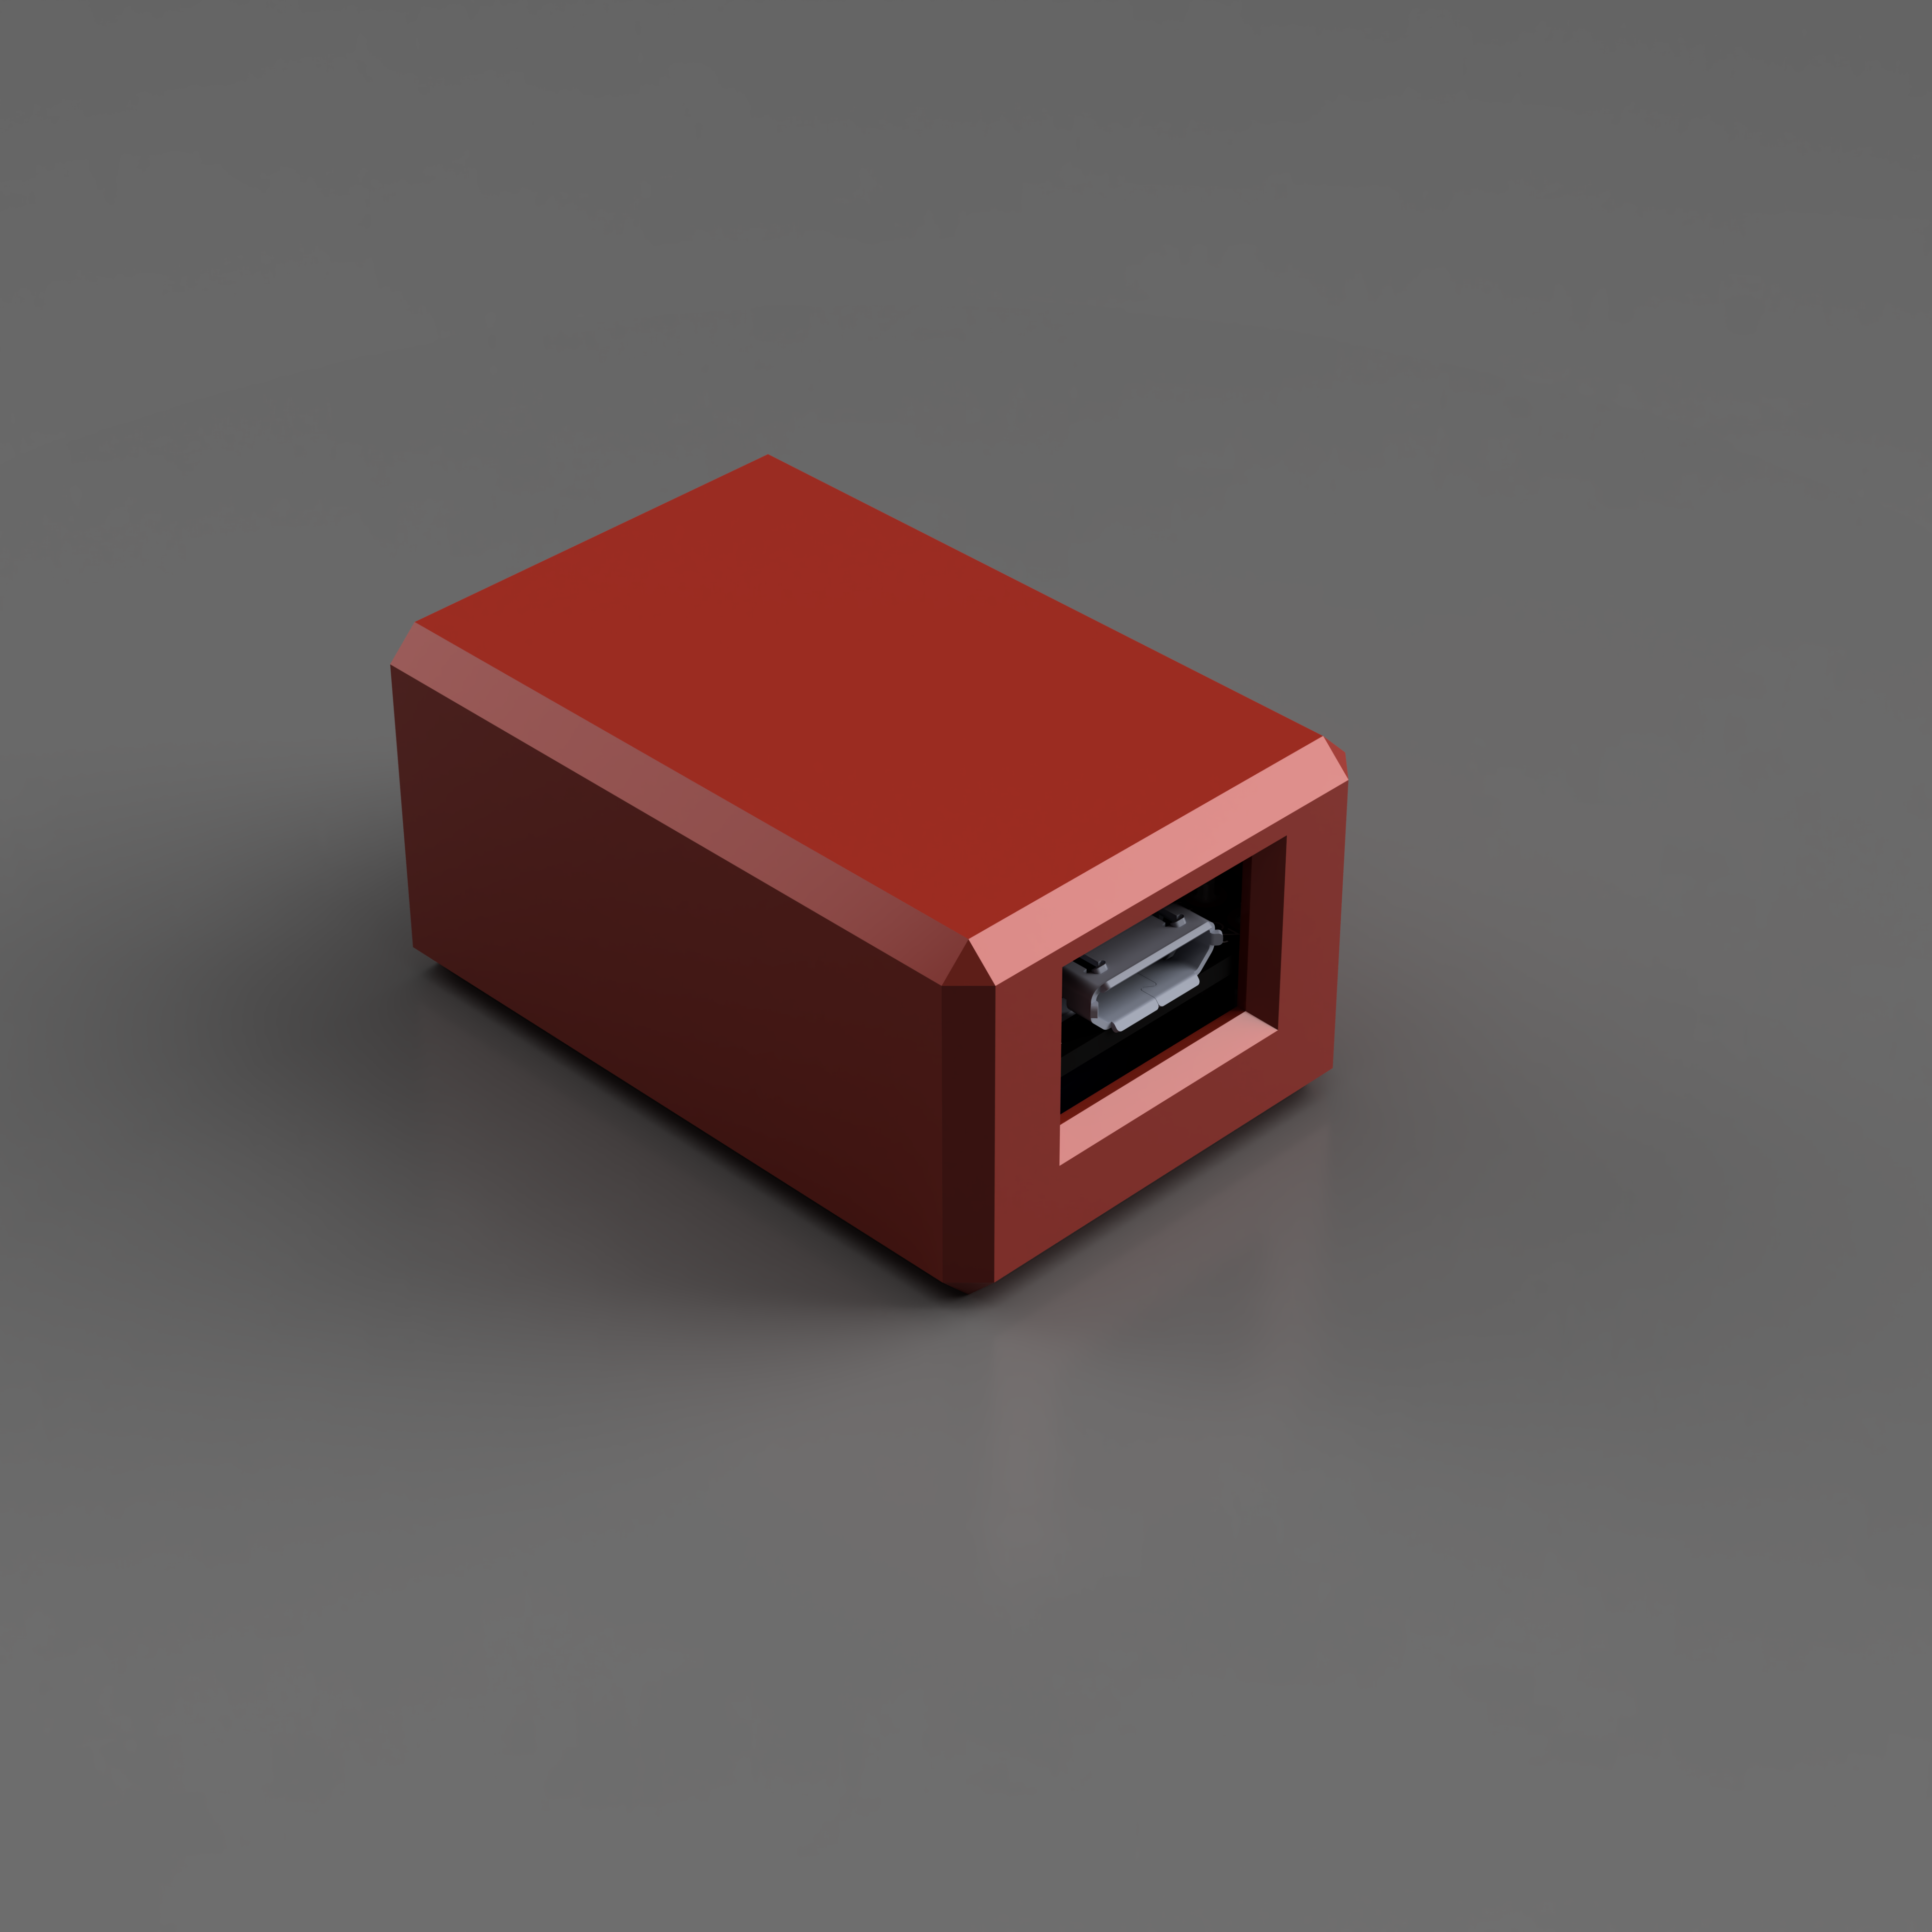
\includegraphics[width=.8\linewidth]{graphics/cad/wearable_1.png}
  \captionsetup{width=0.8\linewidth, justification=centering}
  \centering
  \captionof{figure}{Assembled wearable device}
  \label{fig:wearable_1}
\end{minipage}
\end{figure}

            The wiring and soldering was done prior to assembly, with approximate but accurate measurements of 26awg silicone wire, to allow for a minimal form factor and to fit in the small enclosure. Silicone wire was used to ensure the tight bends and cable management could be achieved.

            \begin{figure}[H]
\centering
\begin{minipage}{.5\textwidth}
  \centering
  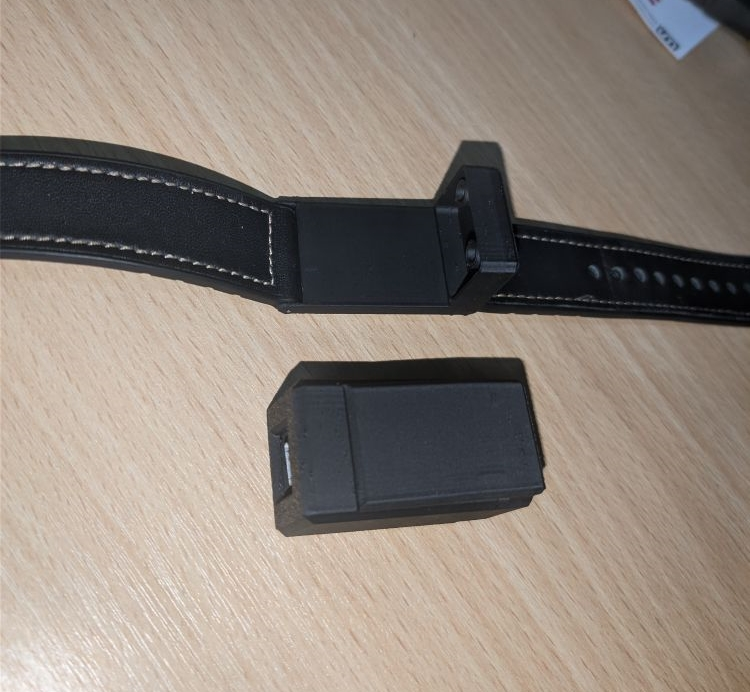
\includegraphics[width=.8\linewidth]{graphics/prototype/attachments.jpeg}
  \captionsetup{width=0.8\linewidth, justification=centering}
  \centering
  \captionof{figure}{Both currently available attachments}
  \label{fig:attachments_1}
\end{minipage}%
\begin{minipage}{.5\textwidth}
  \centering
  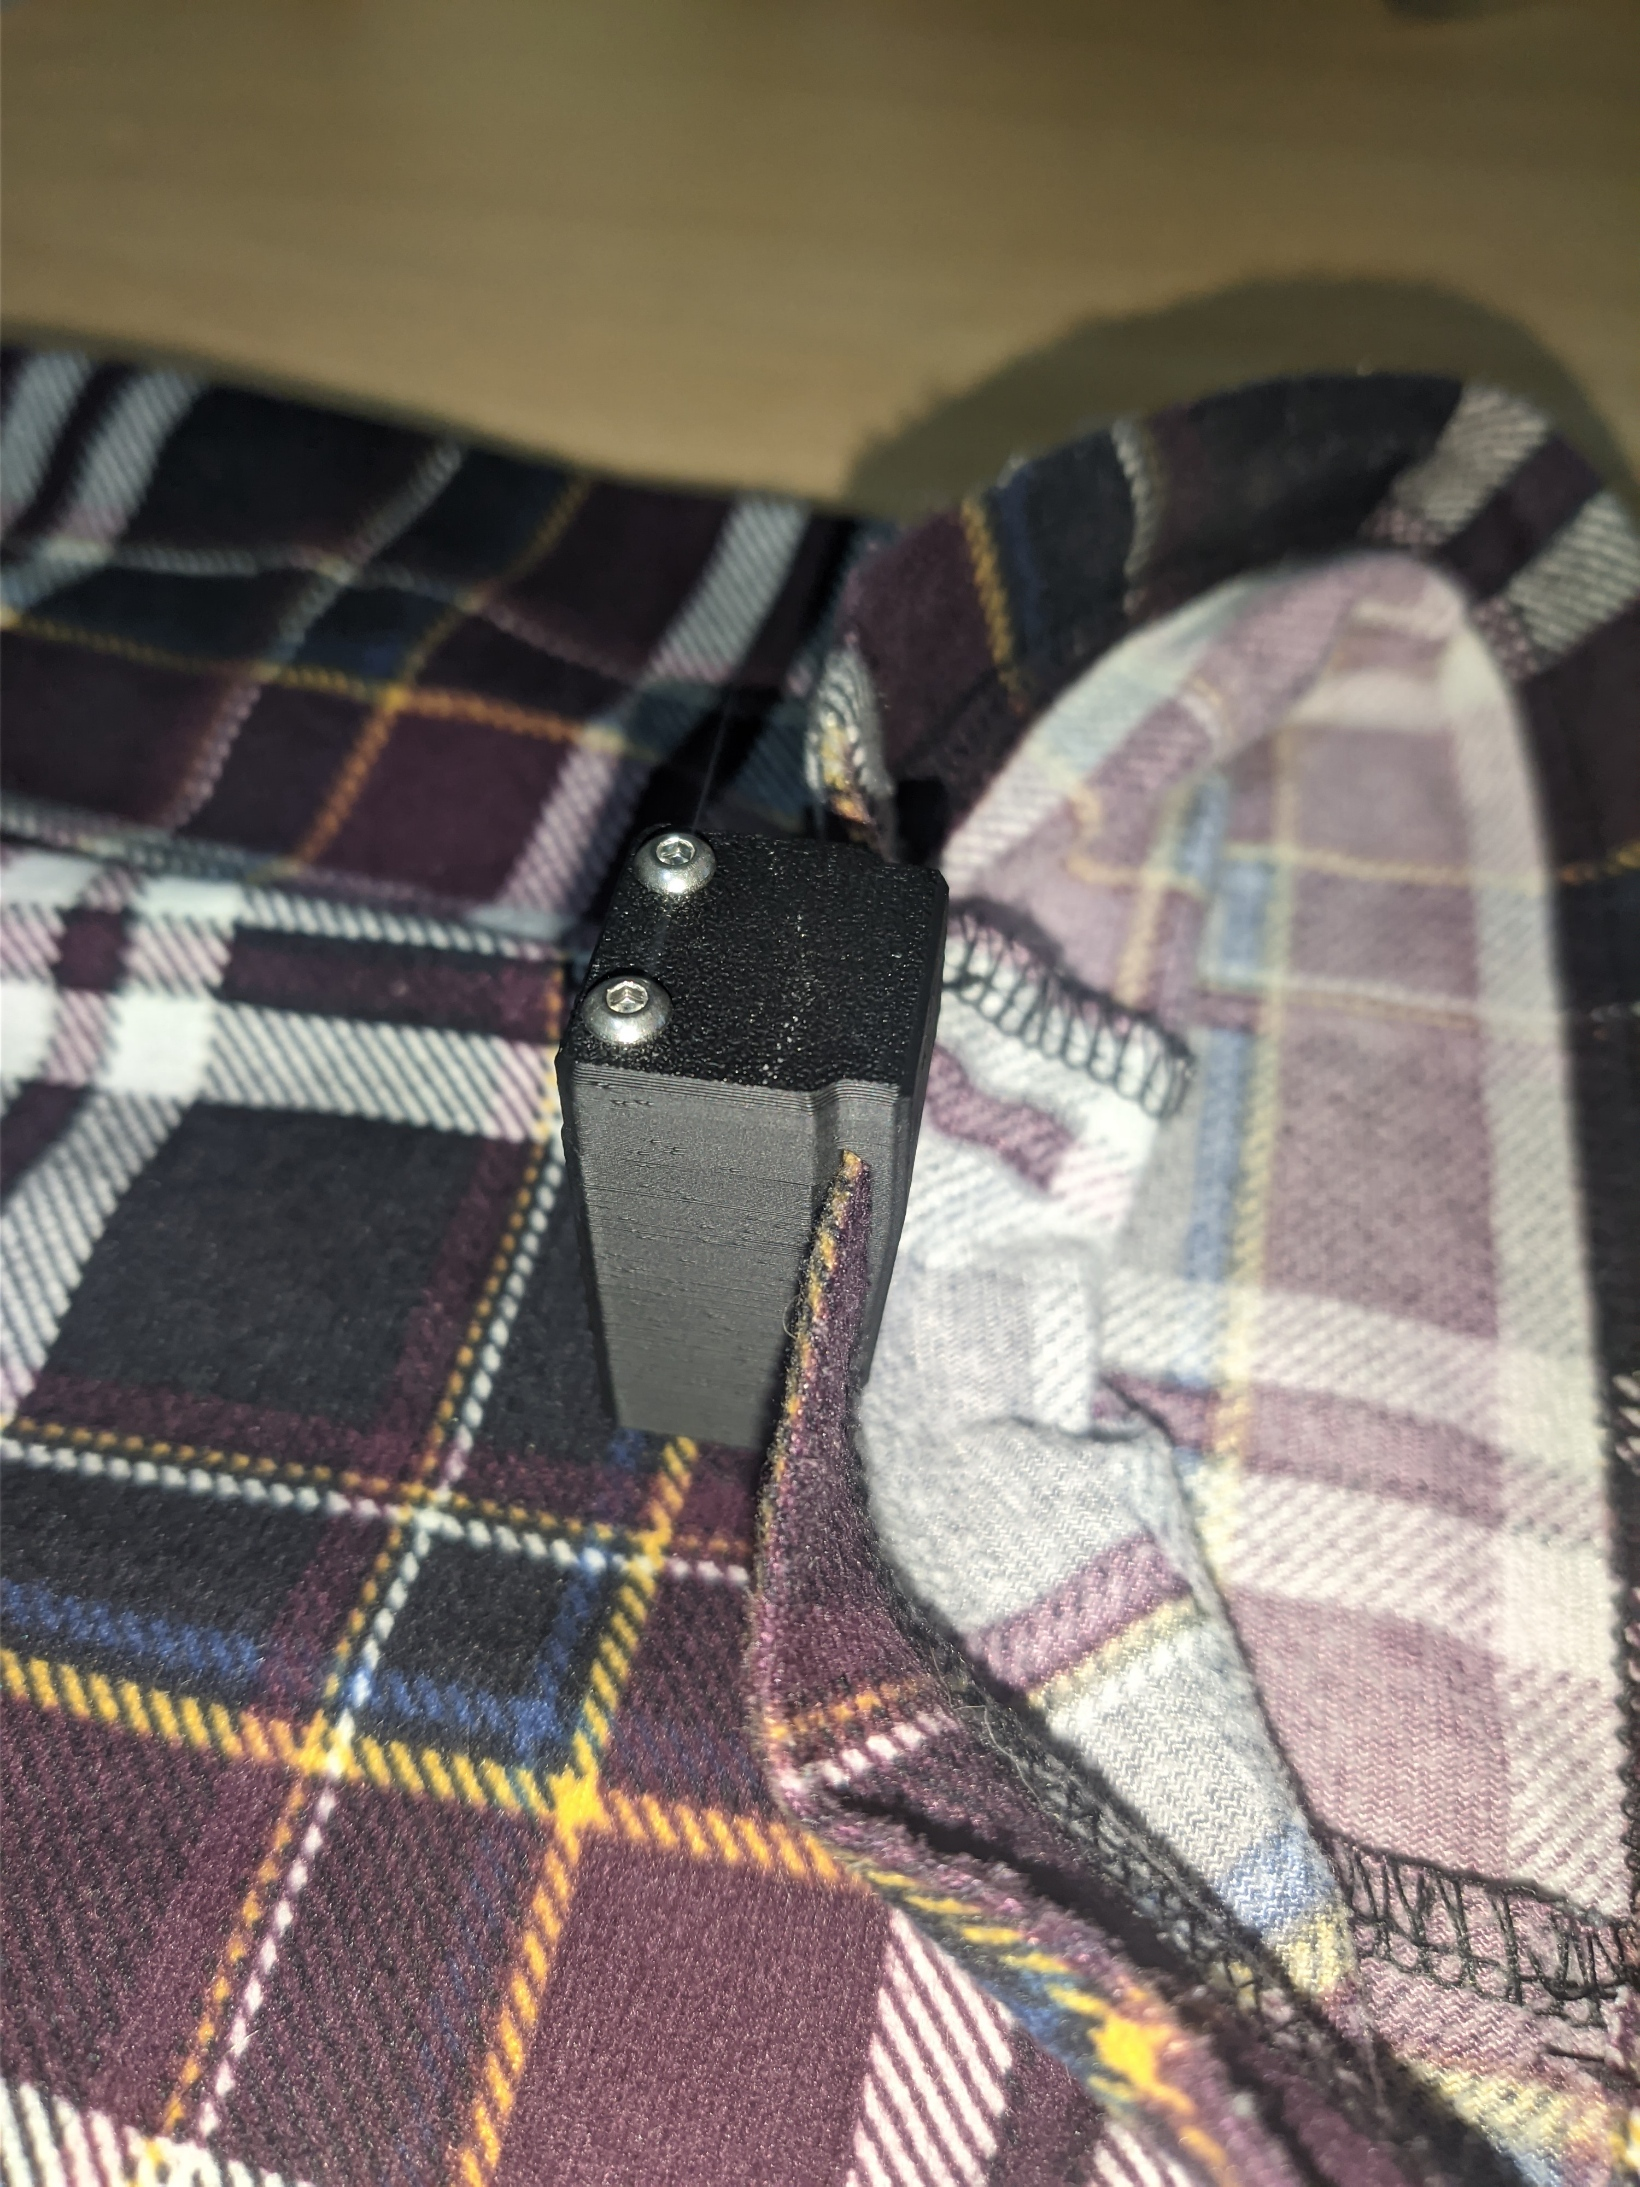
\includegraphics[width=.8\linewidth]{graphics/prototype/attachment_clip.jpg}
  \captionsetup{width=0.8\linewidth, justification=centering}
  \centering
  \captionof{figure}{Clip attachment in use}
  \label{fig:watchstrap_2}
\end{minipage}
\end{figure}

            We have created the two available attachments, as previously described, a clip that can be worn on any existing bands, pockets or clipped directly to clothing/sleeves. Also shown is the watch strap attachment, without the device to show off the geometry of the design

            \begin{figure}[H]
\centering
\begin{minipage}{.5\textwidth}
  \centering
  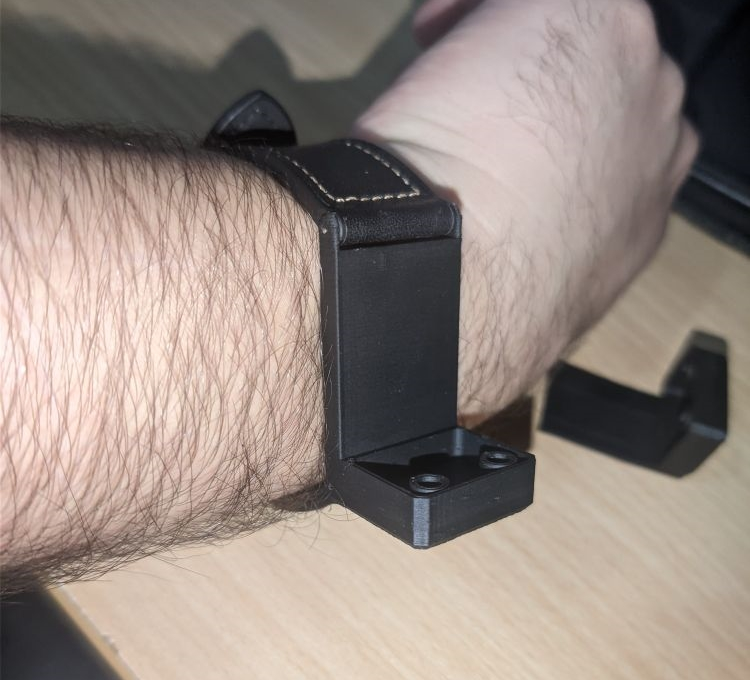
\includegraphics[width=.8\linewidth]{graphics/prototype/wriststrap_1.jpeg}
  \captionsetup{width=0.8\linewidth, justification=centering}
  \centering
  \captionof{figure}{Watchstrap being worn}
  \label{fig:watchstrap_2}
\end{minipage}%
\begin{minipage}{.5\textwidth}
  \centering
  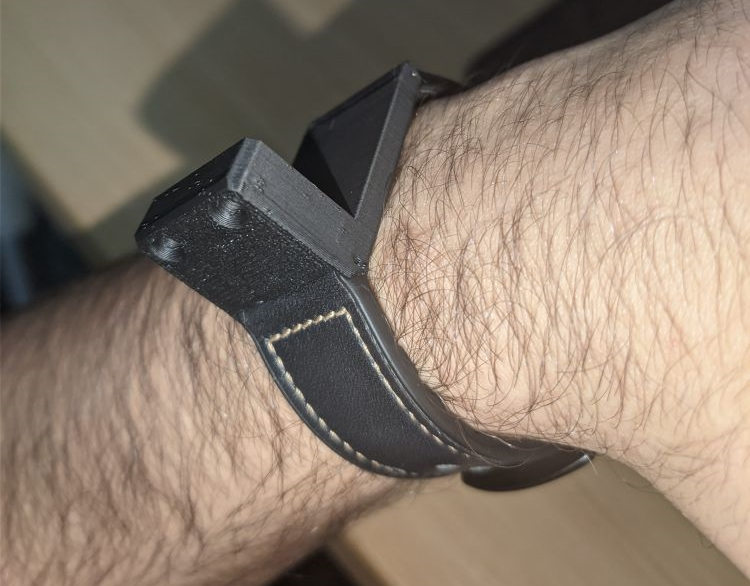
\includegraphics[width=.8\linewidth]{graphics/prototype/wriststrap_2.jpeg}
  \captionsetup{width=0.8\linewidth, justification=centering}
  \centering
  \captionof{figure}{Watchstrap being worn}
  \label{fig:watchstrap_2}
\end{minipage}
\end{figure}

            Shown above is the wrist strap attachment, which allows the use of regular 22mm watch bands, using standard push pin connectors. This allows the patient to be more comfortable, and use existing watch straps they may already own and be accustomed to.



        \subsection{UML}
        \label{sec:uml_wearable}
        
            This section will break down the software systems utilised in the walking aid device into formal language representations. These will take the form of a class diagram, which will illustrate the relationships between each of classes developed for the system, and an activity diagram which will demonstrate the sequence of events that will take place in the system and how they are handled. We hope that this section will help the reader to understand the software system in a broken down, step-by-step manner and to gain an understanding of our rationale towards programming choices that helped us to fulfil the user requirements. The class diagrams will be followed by an explanation of the role of each class and its functions, with the activity diagram also being accompanied by a body of text that establishes in natural language the sequence of events that will take place in the software system and how they are processed.

            \subsubsection{Class Diagram}
            \label{subsubsec:class_diagram_wearable}

                Similarly to the walking aid device section, this section will include the class and activity diagrams of the wearable device. Each diagram will be accompanied by a body of text that explains the diagram in a natural language format.

                \clearpage
                \thispagestyle{empty}
                \begin{landscape}
                    % [H] means put the figure HERE, directly when you input this code.
\begin{figure}[H]
	\centering
	\captionsetup{width=1.0\linewidth}

% We set the width of the figure based on the width of one line of text on the page.
% The value can be tuned to any value in [0.0, 1.0] to scale the image while maintaining its aspect ratio.

	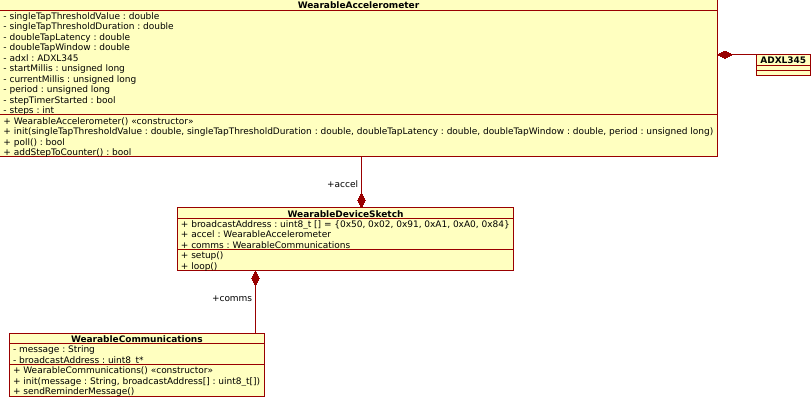
\includegraphics[width=1.0\linewidth]{./UML/WearableDevice/class diagram.png}

% Caption is defined with a short and long version. The short version is shown in the
% List of Figures section, and the long version is used directly with the figure.
	\caption[Wearable Device Class Diagram]{A class diagram for the wearable device software system illustrating how the classes interact with each other.}

% For figures label should be defined after the caption to ensure proper figure numbering.
	\label{fig:class_diagram_wearable}

\end{figure}
                \end{landscape}

                \paragraph{WearableDeviceSketch}\mbox{}

                    This is the main sketch for the wearable device system and implements the setup and loop functions necessary for an Arduino system. It creates instances of the WearableAccelerometer and WearableCommunications class to provide the full functionality of the wearable device. The setup function initialises both classes with the developer's selected parameters. Following this, the loop function handles the calls to check if the user has moved more than 5 steps within a period of time set by the developer. If they have, then the communications object is called to handle the broadcasting of a reminder message to the walking aid device.

                    The WearableDeviceSketch has a composition relationship to both of the other classes as it plays the role of instantiating both objects. Therefore, without the existence of the WearableDeviceSketch, an object of the other two classes would not exist.

                \paragraph{WearableCommunications}\mbox{}

                    The WearableCommunications class handles all the functionality needed to broadcast a message to the walking aid device. Once it is initialised by the WearableDeviceSketch class with a reminder message to send and a MAC address to send the message to, its sendReminderMessage function can be called to broadcast a reminder message when the user has walked more than 5 steps in a specified period of time set by the developer. It is also initialised with the details of the walking aid device as a peer to allow incoming communication. The WearableCommunications class has a composition relationship with the DebugLED class to allow for the LED to be configured should an error occur with the initiation of the communication protocol.

                    This class is also part of a composition relationship with the WearableDeviceSketch class and therefore an object of it cannot exist unless the WearableDeviceSketch class is instantiated.

                \paragraph{DebugLED}\mbox{}

                    The DebugLED class exists to handle the configuration of the TinyPICO's onboard LED to indicate whether the communication protocol is working or not. It is initialised in the WearableDeviceSketch class and is therefore part of a composition relationship with the WearableCommunications class. More specifically, an instance of the DebugLED class cannot exist without an instance of the WearableCommunications class.

                    The DebugLED class also holds a composition relationship with the TinyPICO helper library to allow for the configuration of the LED.

                \paragraph{WearableAccelerometer}\mbox{}

                    Controlling the functionality of the walking detection, this class utilises the ADXL345 accelerometer library to detect single-taps or gravitational changes through the accelerometer. Once it is initialised with threshold values and a value for the period of time used to check for 5 steps, the poll function can be called by the WearableDeviceSketch to check for steps. Each time a step is detected, the addStepToCounter function is called to add to the total number of steps detected. If a step is detected, and it has taken more than the period of time since the first step is detected, then the timer is reset. Otherwise, if the step counter is incremented and is still less than 5 steps, then we move on. However, if the step counter reaches 5 steps within the developer set period of time, then a true boolean value is returned to the WearableDeviceSketch to notify it that a reminder message should be sent to the walking aid device.

                    The class holds a composition relationship with the ADXL345 library to retrieve the necessary functionality for step detection. This class is also part of a composition relationship with the WearableDeviceSketch class, meaning that if an instance of the WearableDeviceSketch class does not exist then neither will an instance of this class. 

                \newpage

            \subsubsection{Activity Diagram}
            \label{subsubsec:wearable_activity}

                The following is an activity diagram that demonstrates the workflow of the wearable software system. The diagram demonstrates how the system attempts to detect that the user is walking in a step-by-step manner to provide clarity of how the software was developed for these purposes. Accompanying the diagram will be a body of text that describes the process in natural language.

                % [H] means put the figure HERE, directly when you input this code.
\begin{figure}[H]
	\centering
	\captionsetup{width=1.0\linewidth}

% We set the width of the figure based on the width of one line of text on the page.
% The value can be tuned to any value in [0.0, 1.0] to scale the image while maintaining its aspect ratio.

	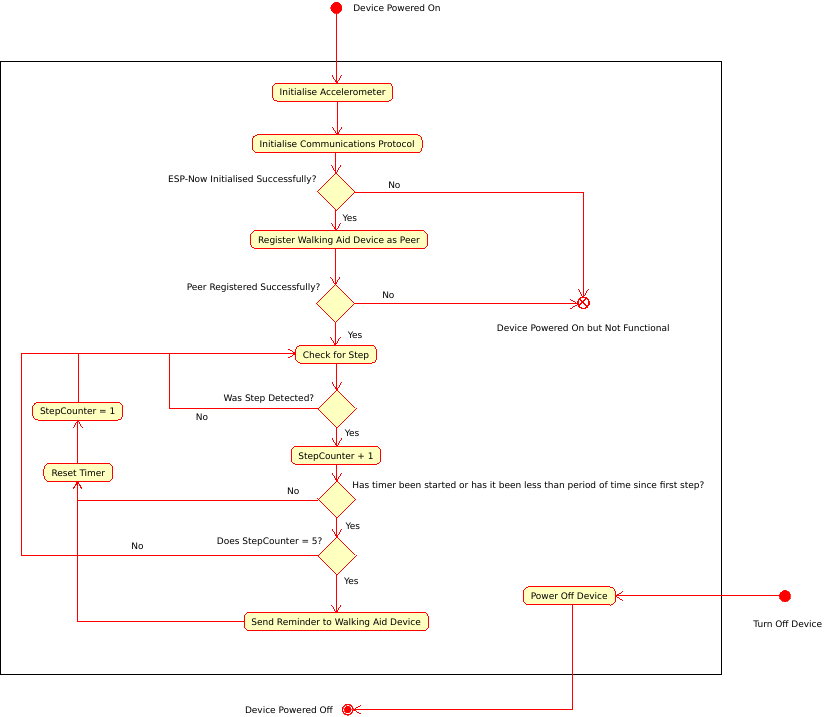
\includegraphics[width=1.0\linewidth]{./UML/WearableDevice/activity diagram.png}

% Caption is defined with a short and long version. The short version is shown in the
% List of Figures section, and the long version is used directly with the figure.
	\caption[Wearable Device Activity Diagram]{An activity diagram for the wearable device software system illustrating the workflow of the system.}

% For figures label should be defined after the caption to ensure proper figure numbering.
	\label{fig:activity_diagram_wearable}

\end{figure}

                The activity diagram demonstrates that the system begins when the device is powered on. The system begins by initialising the accelerometer with the configurations of the developer before attempting to initialise the ESP-Now communications protocol and registering the walking aid device as a peer for communication. If either of ESP-Now steps fail then we end up in a state where the device is powered on but is not functional. 

                If the communication initialisation is successful, then we begin the process of attempting to identify when the user is walking. We begin first by checking for a step, which in actual fact checks if the accelerometer has detected a change in gravity. If it has not detected a step, then we loop back and check for a step again until we identify one. Otherwise, we increment the step counter before checking to see if the timer has started and if it has, then we check to see if the time since the first step was detected is greater than the period of time set by the developer. If the timer has not been started, or it has been greater than the developer specified period of time since the first step, we reset the timer and set the step counter back to 1 and start the check for step process again. Otherwise, we run a check to see if the step counter is now at 5 steps. If it is not, then we loop back to the beginning of the check for step counter. If the step counter is indeed equal to 5, then we have reached the situation where the user has moved a considerable amount in the period of time set by the developer. We can therefore ascertain that the user is walking and send a reminder message to the walking aid device to check if the walking aid is moving as well.

                Finally, despite it not following activity diagram etiquette, we wanted to demonstrate how powering off the system is the only way to stop the device from being functional. The existence of a second initial activity that controls the powering off of the system demonstrates this, and demonstrates how the rest of the system relies on the device being powered on.

    \section{Walking Aid \& Wearable Device Design Commonalities}
    \label{sec:both_devices}

        This section will contain information on the design decisions we made that impacted both the wearable and walking aid devices. This will include software and hardware decisions that allowed us to implement a communications system, that allowed us to keep device form factor and power usage to a minimum, and discussion of why we chose pieces of hardware that are common between both devices.

        \subsection{Development Board - TinyPICO}
        \label{subsec:development_board}

            The development board for each device would provide the necessary communication between multiple hardware components to allow us to reach the originally defined user requirements. Due to our previous experience with ESP32 chips and due to the necessity of our devices being of a small enough form factor to fit on the limbs of patients and on walking aids, we decided to use the TinyPICO development boards. Their use of ESP32 chips provide the basis for our communication system which utilises a Wi-Fi module, and provides adequate pin outs to allow us to communicate to each hardware device that we include within our systems. This is all achieved whilst keeping power usage to a minimum and allowing us to meet the client requirement of creating devices that are able to operate for a substantial amount of time without the need for battery replacements. The 240MHz dual-core chip that is the ESP32, would provide performance that allows our system to react to incoming communication from the Wi-Fi module or accelerometer promptly to provide a responsive system for our clients. The vast documentation supporting the development of embedded systems using ESP32s was instrumental in the success of our project, and we feel that the decision to utilise TinyPICO development boards was the correct one because of it. We were also influenced to use TinyPICO development boards due to Swansea University allowing us to borrow two boards at no extra cost, which ultimately allowed us to remain within our £150 budget. Finally, the TinyPICO boards also provide a built-in LED which we utilised throughout project development for debugging purposes.

        \subsection{Programming Language - Arduino C (C/C++)}
        \label{subsec:programming_language}

            We decided to utilise the Arduino C (C++) programming language rather than using MicroPython to develop our embedded software due to C++'s superior efficiency over Python for the development of embedded software \cite{github_2014, dicola}. Other tools such as PlatformIO would have provided the basis to allow us to utilise C++ for our software development, but due to the benefits of our team having previous experience of using the Arduino IDE to develop embedded systems, especially in the field of software development with ESP32 chips, we felt that our project would be better suited to being developed utilising the Arduino ecosystem. We were also aware that the handover of this project would mean that another team would be able to take on the role of advancing our code and felt that C++ provided the best platform for developing smaller and more self-explanatory code across multiple header and implementation files. This would mean that any developers that attempt to further develop our code in future, should find it rather simple to identify what each class and block of code is attempting to accomplish.

        \subsection{Accelerometer - Adafruit ADXL345}
        \label{subsec:accel}

            Within this project, the accelerometer would provide the basis for identifying movement of the patient and the walking aid. The vast documentation supporting the development of embedded systems using ADXL345 accelerometers was a substantial factor in why we opted to include them in our systems. They provide the functionality for the detection of various changes in acceleration such as activity detection, free fall detection and single-tap and double-tap detection. The single-tap detection feature of the ADXL345 provides the basis for movement detection on both devices due to the fact that it can detect changes in gravity to identify when a step has been taken. The single-tap detection feature also allows the system to still be utilised whether the user is wearing the wearable device on their wrist or ankle, with the single-tap detection feature also being able to detect when the walking aid is being lifted and placed back on the ground. The free fall detection feature provided by the ADXL means that future developers will be able to easily implement a free fall detection system, which would allow the client to have their stretch goal implemented into the project. We opted to use the ADXL345 over other accelerometers as it is one of the newer offerings of accelerometers from the well renowned and reliable brand, Adafruit. Because of this, the accelerometers were relatively easy and quick to source, whilst only costing £7 per unit and allowing us to remain within our £150 budget. Finally, with the walking aid's TinyPICO already having its Serial Peripheral Interface and 3.3V power pin outs being utilised by the I2S audio shield, the ADXL345 allowed us to use the TinyPICO's I\textsuperscript{2}C interface for communication between the accelerometer and the development board, and allowed us to use the 5V pin out provided by the TinyPICO to power the ADXL345 due to its built-in voltage regulator.

        \subsection{Communication Protocol - ESP-Now}
        \label{subsec:esp_now_comms}

            Within the details specified in our Milestone 2 interim progress report, we classified the advantages and disadvantages of various options for communication protocols for use within our project. The first of those communication protocols was ESP-Now, a communication technology developed by the creators of the ESP32 chip, Espressif, which utilises the ESP32's Wi-Fi module to communicate with other devices that contain ESP32 chips \cite{esp-now_overview}. The other two communication protocol options we could have utilised were Bluetooth Low Energy (BLE) and Ultra-wideband (UWB). Despite considerations to include the use of UWB within our project, it would have been far too expensive for us to implement, and thus we instantly rejected the notion of using UWB within our project. Therefore, we were left with a decision to either utilise BLE or ESP-Now for the communication standard between our walking aid and wearable device. For the rest of this section, we will detail the advantages and disadvantages to using ESP-Now for our communication system, with comparisons to BLE, before finally detailing why we ultimately opted to utilise ESP-Now.

            \newpage
            \subsubsection{Advantages and Disadvantages of ESP-Now with comparisons to BLE}
            \label{subsubsec:esp_now_advantages_disadvantages}

                \vspace{2em}
                \small
		\begin{xltabular}[H]{\textwidth}{p{0.47\textwidth} | p{0.47\textwidth}}
			\caption[ESP-Now Advantages and Disadvantages]{A table listing the advantages and disadvantages of the ESP-Now protocol.}\\

			\toprule

		 	Advantages & Disadvantages\\

			\midrule
			\endfirsthead

			\toprule

			Advantages & Disadvantages\\

			\midrule
			\endhead

			\hline
			\multicolumn{2}{|r|}{{Continued on next page}}\\
			\hline
			\endfoot

			\bottomrule
			\endlastfoot

			Provides a simple implementation of two-way communication between ESP32s \cite{random_nerd_tutorials}. This would allow us to easily send messages between the wearable and walking aid device to check if either are moving.
			
			&
			
			Similar to UWB, it is only adoptable for ESP chips and therefore less adopted in this area than BLE, meaning we will be limited to using ESP chipped boards for future product development, or we would have to redevelop our communication system.\\
			
			\midrule
			
			Maximum message sizes are limited to 250 bytes \cite{random_nerd_tutorials}. Similar to the advantage stated with BLE, a small message size means minimal overheads, which is beneficial to our project as we will only be sending short signal messages between devices.
			
			&
			
			ESP-Now is less power efficient than BLE \cite{neupane_2019} and in turn less power efficient than UWB \cite{bender_2021}. This would mean that the patient or carer would need to remember to change the batteries in our devices more often.\\
			
			\midrule
			
			The ESP-Now library includes callbacks \cite{random_nerd_tutorials} that can allow our devices to notice whether their messages to the other devices have been received successfully or not. This can create a more robust communication protocol that attempts to avoid lost packets. This will mean that reminders that should be played to the patient are less likely to fail.
			
			&
			
			\\
			
			\midrule
			
			ESP-Now was developed for the ESP32 chips found on our TinyPICO boards. Because of this, the documentation provided that directly relates to our hardware is perfect for code development and lessens the difficulty of developing our communication protocol.
			
			&
			
			\\

		\end{xltabular} 
		\label{tbl:now}
                \vspace{5em}

                We ultimately decided to use ESP-Now as our communication protocol due to its ease of implementation and due to the fact that it allows sketch sizes to be smaller \cite{random_nerd_tutorials} than the sketch sizes of BLE \cite{kolban_2018}. The significance to sketch sizes being smaller is that they allow for the larger memory storage spaces accounting for larger audio reminder files, as well as providing more responsive code for what is a time sensitive system. The lower throughput that ESP-Now provides in comparison to BLE should not be noticeable within our system due to the fact that we only ever send one word messages between our devices at a given time. However, the lower power efficiency of ESP-Now in comparison to BLE is a considerable disadvantage for use within this system. Having said this, ESP-Now is still regarded as being a low power solution and should still mean that the patient or carer will not need to remember to replace the batteries in their devices too often.


        \subsection{Power}
        \label{subsec: Power}
            Our prototypes will not include any battery or portable power source support built in, this decision was made due to the limited time and budget we had. Our vision, research and hardware supports 1S Lithium Polymer (LiPo) batteries as standard, and the TinyPico is designed to be used with this power source in mind. Unfortunately, researching safe battery charging circuits as well as proper battery care was not something we had the time for, and will leave as an attainable stretch goal if this project were to gain further funding or time budgets.

            1S LiPos are compact, and offer excellent discharge currents which would make it ideal for our high wattage speaker, although adjusting speaker size can reduce the battery requirement quite significantly, and can be considered later on with further research and testing.

            Our prototypes are powered by the same MicroUSB, 5V port that is used for programming and updating the device, to facilitate testing, these will run off of portable power banks with USB outputs, to ensure reliable voltage and amperage is provided to our devices to reduce potential issues during testing.

        \subsection{Prototyping}
        \label{subsec: Prototyping}
        
            The software package used for designing the prototypes was chosen to be Autodesk Fusion 360 \cite{autodesk_2021}, as well as how pervasive it is within the 3D Printing community.

            Where possible, we ensured to use accurate existing models. This allowed us to make progress faster, as working out and modelling tight tolerances on PCB components wasn't always required. 

            For the hardware we could not find models for, such as the speaker, i2s audio shield, and vibration motor, critical dimensions were taking using Vernier calipers, and by cross checking datasheets for each or similar devices.

            For both devices, a large emphasis was placed on creating an enclosure for the electronics with a minimal, but modular form factor. As shown in their respective sections, the devices were designed to effectively house and protect the existing components, as well as allow for future expansion using modular systems and design choices, such as extendable mid plates and standard sized screws and fasteners.

            Once designs for the enclosures were created, they were sliced and converted to gcode (file format used by 3D Printers, CNC routers, and other kinematic machines) using the open source software package SuperSlicer \cite{merill_2022}, and then printed on a custom VoronDesign 0.1 CoreXY Fused Filament Deposition (FDM) 3D Printer. SuperSlicer was chosen due to our teams experience with the software, as well as already having a previously tuned profile for the machine.

            The material for printing was chosen to be Acrylonitrile butadiene styrene (ABS), a ubiquitous thermoplastic most often used with injection moulding in everyday objects due to its high impact resistance and thermal/checmical resistance. It used to be the plastic of choice for hobby grade 3D Printing, however is becoming less common vs easier to print, and weaker/biodegradable plastics like Polylactic Acid (PLA) or Polyethylene terephthalate (PETG). We chose to continue with ABS, as our printer is cable of printing this more exotic material, and its properties will us to undertaken stricter impact and resistance testing.             
        
    \newpage

    \section{Class Documentation - Walking Aid Device}
    \label{sec:class_documentation_walk_aid}\mbox{}

        \subsection{SDToSPIFFS Class Reference}
        \label{subsec:sdtospiffs}\mbox{}

                \paragraph{Public Member Functions}\mbox{}

                    \begin{itemize}
                        \item \textbf{SDToSPIFFS}() 
                        
                            \textit{Construct a new SDToSPIFFS object.}

                        \item void \textbf{init}(const char *SDPath, const char* SPIFFSPath) 
                        
                            \textit{Initalises the object ready for the transferring of files from SD card to SPIFFS.}

                        \item \textbf{loadSDFileToSPIFFS}() 
                        
                            \textit{Handles the loading of the SD card file to SPIFFS.}

                        \item const char *\textbf{getSPIFFSPath}() 
                        
                            \textit{Returns the path to the SPIFFS file.}
                    \end{itemize}

            \subsubsection{Member Function Documentation}\mbox{}

                \paragraph{SDToSPIFFS()}\mbox{}\\

                    \ttfamily{SDToSPIFFS::SDToSPIFFS (  )}\\

                    \rmfamily{Construct a new SDToSPIFFS object.}

                \paragraph{init()}\mbox{}\\

                    \ttfamily{void SDToSPIFFS::init (\\
                        \null \quad \quad \quad \quad \quad \quad \quad \quad \quad const char * SDPath,\\ 
                        \null \quad \quad \quad \quad \quad \quad \quad \quad \quad const char * SPIFFSPath )}\\

                    \rmfamily{Returns the path to the SPIFFS file.}

                    \textbf{Parameters}

                    \vspace{1em}
                    \begin{tabular}{| l | l |} 
                        \hline
                        SDPath & The path to the SD card file. \\ 
                        \hline
                        SPIFFSPath & The file name to give the new SPIFFS file. \\ 
                        \hline
                    \end{tabular}

                \paragraph{loadSDFileToSPIFFS()}\mbox{}\\

                    \ttfamily{void SDToSPIFFS::loadSDFileToSPIFFS (  )}\\
    
                    \rmfamily{Handles the loading of the SD card file to SPIFFS.}

                \paragraph{getSPIFFSPath()}\mbox{}\\

                    \ttfamily{const char * SDToSPIFFS::getSPIFFSPath (  )}\\

                    \rmfamily{Returns the path to the SPIFFS file.}

                    \textbf{Returns}

                        \quad \quad const char* SPIFFS file path.
        \newpage
        \subsection{WalkAidAccelerometer Class Reference}
\label{subsec:WalkAidAccelerometer}\mbox{}

    \ttfamily{}

    \#include <WalkAidAccelerometer.h>\\

    \rmfamily{}

    \paragraph{Private Attributes}\mbox{}\\

        \begin{itemize}
            \item double \textbf{singleTapThresholdValue}
            
                \quad \quad \textit{Threshold for single tap to be detected.}

            \item double \textbf{singleTapThresholdDuration}
            
                \quad \quad \textit{Duration for single tap to be above threshold to be detected.}

            \item double \textbf{doubleTapLatency}
            
                \quad \quad \textit{Time between a tap event and when the reading for a double tap starts.}

            \item double \textbf{doubleTapWindow}
            
                \quad \quad \textit{Defines how long a double tap is checked for.}

            \item bool \textbf{stepDetected}
            
                \quad \quad \textit{Defines if a step has been detected.}

            \item long \textbf{lastStepTime}
            
                \quad \quad \textit{The last time a step was detected.}

            \item unsigned long \textbf{period}
            
                \quad \quad \textit{The period to check previously and in future for detected steps.}

            \item ADXL345 \textbf{adxl}
            
                \quad \quad \textit{Accelerometer object.}\\

        \end{itemize}


    \paragraph{Public Member Functions}\mbox{}\\

        \begin{itemize}
            \item \textbf{WalkAidAccelerometer}() 
            
                \quad \quad \textit{Construct a new Walk Aid Accelerometer object.}

            \item void \textbf{init}(double singleTapThresholdValue, double singleTapThresholdDuration
            , \\double doubleTapLatency, double doubleTapWindow, unsigned long period) 
            
                \quad \quad \textit{Initialises the accelerometer with the specified values in parameter fields.}

            \item bool \textbf{checkForStep}() 
            
                \quad \quad \textit{Checks if a tap event was detected by the accelerometer.}

            \item bool \textbf{isStepDetected}() 
            
                \quad \quad \textit{Returns the value of stepDetected.}

            \item long \textbf{getLastStepTime}() 
            
                \quad \quad \textit{Get the time the last step was taken.}

            \item unsigned long \textbf{getPeriod}() 
            
                \quad \quad \textit{Get the developer's specified period to check for steps.}\\

        \end{itemize}

    \subsubsection{Constructor \& Destructor Documentation}\mbox{}


        \paragraph{WalkAidAccelerometer()}\mbox{}\\

            \ttfamily{WalkAidAccelerometer::WalkAidAccelerometer (  )}\\

            \rmfamily{Construct a new Walk Aid Accelerometer object.}\\


    \subsubsection{Member Function Documentation}\mbox{}


        \paragraph{init()}\mbox{}\\

            \ttfamily{void WalkAidAccelerometer::init (\\
                \null \quad \quad \quad \quad \quad \quad \quad \quad \quad double singleTapThresholdValue,\\ 
                \null \quad \quad \quad \quad \quad \quad \quad \quad \quad double singleTapThresholdDuration,\\ 
                \null \quad \quad \quad \quad \quad \quad \quad \quad \quad double doubleTapLatency,\\
                \null \quad \quad \quad \quad \quad \quad \quad \quad \quad double doubleTapWindow,\\
                \null \quad \quad \quad \quad \quad \quad \quad \quad \quad unsigned long period)}\\

            \rmfamily{Initialises the accelerometer with the specified values in parameter fields.}

            \textbf{Parameters}

            \vspace{1em}
            \begin{tabular}{| l | l |} 
                \hline
                singleTapThresholdValue & Threshold for single tap to be detected.\\ 
                \hline
                singleTapThresholdDuration & Duration that tap must be above threshold to be detected.\\ 
                \hline
                doubleTapLatency & Time after single tap until double tap is measured.\\ 
                \hline
                doubleTapWindow & How long double tap is checked for.\\ 
                \hline
                period & Time period to check for steps before and after receiving message.\\ 
                \hline
            \end{tabular}\\~\\


        \paragraph{checkForStep()}\mbox{}\\

            \ttfamily{bool WalkAidAccelerometer::checkForStep (  )}\\

            \rmfamily{Checks if a tap event was detected by the accelerometer.}\\

            \textbf{Returns}

                \quad \quad true if tap is detected, false otherwise.\\


        \paragraph{isStepDetected()}\mbox{}\\

            \ttfamily{bool WalkAidAccelerometer::isStepDetected (  )}\\

            \rmfamily{Returns the value of stepDetected.}

            \textbf{Returns}

                \quad \quad bool stepDetected\\

        \paragraph{getLastStepTime()}\mbox{}\\

            \ttfamily{long WalkAidAccelerometer::getLastStepTime (  )}\\

            \rmfamily{Get the time the last step was taken.}

            \textbf{Returns}

                \quad \quad long lastStepTime.\\

        \paragraph{getPeriod()}\mbox{}\\

            \ttfamily{unsigned long WalkAidAccelerometer::getPeriod (  )}\\

            \rmfamily{Get the developer's specified period to check for steps.}

            \textbf{Returns}

                \quad \quad unsigned long period.\\
        \newpage
        \subsection{WalkAidAudio Class Reference}
\label{subsec:WalkAidAudio}\mbox{}

    \ttfamily{}

    \#include <WalkAidAudio.h>\\

    \rmfamily{}

    \paragraph{Private Attributes}\mbox{}\\

        \begin{itemize}
            \item AudioGeneratorMP3 * \textbf{mp3}
            
                \quad \quad \textit{The generator of the mp3 player.}

            \item AudioFileSourceSPIFFS * \textbf{file}
            
                \quad \quad \textit{The source file of the SPIFFS audio file.}

            \item AudioOutputI2S * \textbf{out}
            
                \quad \quad \textit{The output of the mp3 player.}

            \item AudioFileSourceID3 * \textbf{id3}
            
                \quad \quad \textit{Metadata handler for the mp3 file.}

            \item SDToSPIFFS \textbf{s2s}
            
                \quad \quad \textit{Object to handle the SD to SPIFFS transfer.}\\

        \end{itemize}


    \paragraph{Public Member Functions}\mbox{}\\

        \begin{itemize}
            \item \textbf{WalkAidAudio}() 
            
                \quad \quad \textit{Construct a new Walk Aid Audio object.}

            \item void \textbf{init}(const char *SDPath, const char *SPIFFSPath) 
            
                \quad \quad \textit{Initialises the accelerometer with the specified values in parameter fields.}

            \item void \textbf{play}() 
            
                \quad \quad \textit{Plays the SPIFFS audio file.}\\

        \end{itemize}

    \subsubsection{Constructor \& Destructor Documentation}\mbox{}


        \paragraph{WalkAidAudio()}\mbox{}\\

            \ttfamily{WalkAidAudio::WalkAidAudio (  )}\\

            \rmfamily{Construct a new Walk Aid Audio object.}\\


    \subsubsection{Member Function Documentation}\mbox{}


        \paragraph{init()}\mbox{}\\

            \ttfamily{void WalkAidAudio::init (\\
                \null \quad \quad \quad \quad \quad \quad \quad \quad \quad const char * SDPath,\\ 
                \null \quad \quad \quad \quad \quad \quad \quad \quad \quad const char * SPIFFSPath)}\\

            \rmfamily{Initialises the walk aid audio system by calling the transfer of SD file to SPIFFS and generating the}

            mp3 code.

            \textbf{Parameters}

            \vspace{1em}
            \begin{tabular}{| l | l |} 
                \hline
                SDPath & Path to the SD card audio file.\\ 
                \hline
                SPIFFSPath & Name of the SPIFFS audio file to be created.\\ 
                \hline
            \end{tabular}\\~\\


        \paragraph{play()}\mbox{}\\

            \ttfamily{void WalkAidAudio::play (  )}\\

            \rmfamily{Plays the SPIFFS audio file.}\\
        \newpage
        \subsection{WalkAidCommunications Class Reference}
\label{subsec:WalkAidCommunications}\mbox{}

    \ttfamily{}

    \#include <WalkAidCommunications.h>\\

    \rmfamily{}

    \paragraph{Private Attributes}\mbox{}\\

        \begin{itemize}
            \item bool \textbf{reminder}
            
                \quad \quad \textit{Whether a reminder message has been received.}\\

        \end{itemize}


    \paragraph{Public Member Functions}\mbox{}\\

        \begin{itemize}
            \item \textbf{WalkAidCommunications}() 
            
                \quad \quad \textit{Construct a new Walk Aid Communications object.}

            \item void \textbf{init}()
            
                \quad \quad \textit{Initialise communication to the wearable device.}

            \item bool \textbf{getReminder}() 
            
                \quad \quad \textit{Get whether a reminder has been received or not.}
                
            \item void \textbf{setReminder}(bool reminder) 
            
                \quad \quad \textit{Set whether a reminder has been received or not.}\\

        \end{itemize}

    \subsubsection{Constructor \& Destructor Documentation}\mbox{}


        \paragraph{WalkAidCommunications()}\mbox{}\\

            \ttfamily{WalkAidCommunications::WalkAidCommunications (  )}\\

            \rmfamily{Construct a new Walk Aid Communications object.}\\


    \subsubsection{Member Function Documentation}\mbox{}


        \paragraph{init()}\mbox{}\\

            \ttfamily{void WalkAidCommunications::init ()}\\

            \rmfamily{Initialise communication to the wearable device.}

        \paragraph{getReminder()}\mbox{}\\

            \ttfamily{bool WalkAidCommunications::getReminder (  )}\\

            \rmfamily{Get whether a reminder has been received or not.}

            \textbf{Returns}

                \quad \quad bool reminder.\\


        \paragraph{setReminder()}\mbox{}\\

            \ttfamily{void WalkAidCommunications::setReminder (  )}\\

            \rmfamily{Set whether a reminder has been received or not.}

            \textbf{Parameters}

            \vspace{1em}
            \begin{tabular}{| l | l |} 
                \hline
                reminder & true if reminder received, false otherwise.\\ 
                \hline
            \end{tabular}\\~\\
        \newpage
        \subsection{DebugLED Class Reference}
\label{subsec:debugled2}\mbox{}

    \ttfamily{}

    \#include <DebugLED.h>\\

    \rmfamily{}

    \paragraph{Private Attributes}\mbox{}\\

        \begin{itemize}
            \item TinyPICO \textbf{tp}
            
                \quad \quad \textit{The TinyPICO object used to control the LEDs.}\\

        \end{itemize}


    \paragraph{Public Member Functions}\mbox{}\\

        \begin{itemize}
            \item \textbf{DebugLED}() 
            
                \quad \quad \textit{Construct a new DebugLED object.}

            \item void \textbf{poweredOn}() 
            
                \quad \quad \textit{Displays a green LED for 1 second to signify successful power on.}

            \item void \textbf{initError}() 
            
                \quad \quad \textit{Displays a red LED to signify ESP-Now init error.}

            \item void \textbf{peerSetupError}() 
            
                \quad \quad \textit{Displays an orange LED to signify an ESP-Now peer connection error.}\\
        \end{itemize}

    \subsubsection{Constructor \& Destructor Documentation}\mbox{}


        \paragraph{DebugLED()}\mbox{}\\

            \ttfamily{DebugLED::DebugLED (  )}\\

            \rmfamily{Construct a new DebugLED object.}\\


    \subsubsection{Member Function Documentation}\mbox{}


        \paragraph{poweredOn()}\mbox{}\\

            \ttfamily{void DebugLED::poweredOn (  )}\\

            \rmfamily{Displays a green LED for 1 second to signify successful power on.}\\


        \paragraph{initError()}\mbox{}\\

            \ttfamily{void DebugLED::initError (  )}\\

            \rmfamily{Displays a red LED to signify ESP-Now init error.}\\


        \paragraph{peerSetupError()}\mbox{}\\

            \ttfamily{void DebugLED::peerSetupError (  )}\\

            \rmfamily{Displays an orange LED to signify an ESP-Now peer connection error.}\\
        \newpage
        \subsection{Sketch Class Reference}
\label{subsec:sketch}\mbox{}

    \paragraph{Public Attributes}\mbox{}\\

        \begin{itemize}
            \item String \textbf{message}
            
                \quad \quad \textit{A copy of the message received from the wearable device.}

            \item WalkAidAudio \textbf{audio}
            
                \quad \quad \textit{The audio controller object.}

            \item WalkAidCommunications \textbf{comms}
            
                \quad \quad \textit{The communications controller object.}
                
            \item WalkAidAccelerometer \textbf{accel}
            
                \quad \quad \textit{The accelerometer controller object.}\\

        \end{itemize}


    \paragraph{Public Member Functions}\mbox{}\\

        \begin{itemize}
            \item void \textbf{setup}() 
            
                \quad \quad \textit{Handles the Arduino setup function. Initialises the accelerometer, communications, and audio.}

            \item void \textbf{loop}() 
            
                \quad \quad \textit{Handles the Arduino loop function. Loops through checks for reminder messages and responds accordingly.}\\
        \end{itemize}


    \subsubsection{Member Function Documentation}\mbox{}


        \paragraph{setup()}\mbox{}\\

            \ttfamily{void setup (  )}\\

            \rmfamily{Handles the Arduino setup function. Initialises the accelerometer, communications, and audio.}


        \paragraph{loop()}\mbox{}\\

            \ttfamily{void loop (  )}\\

            \rmfamily{Handles the Arduino loop function. Loops through checks for reminder messages and responds accordingly.}\\
        \newpage

    \section{Class Documentation - Wearable Device}
    \label{sec:class_documentation_wearable}\mbox{}

        \subsection{WearableAccelerometer Class Reference}
\label{subsec:WearableAccelerometer}\mbox{}

    \ttfamily{}

    \#include <WearableAccelerometer.h>\\

    \rmfamily{}

    \paragraph{Private Attributes}\mbox{}\\

        \begin{itemize}
            \item double \textbf{singleTapThresholdValue}
            
                \quad \quad \textit{Threshold for single tap to be detected.}

            \item double \textbf{singleTapThresholdDuration}
            
                \quad \quad \textit{Duration for single tap to be above threshold to be detected.}

            \item double \textbf{doubleTapLatency}
            
                \quad \quad \textit{Time between a tap event and when the reading for a double tap starts.}

            \item double \textbf{doubleTapWindow}
            
                \quad \quad \textit{Defines how long a double tap is checked for.}

            \item ADXL345 \textbf{adxl}
            
                \quad \quad \textit{Accelerometer object.}

            \item unsigned long \textbf{startMillis}
            
                \quad \quad \textit{Keeps track of when the first step was taken.}

            \item unsigned long \textbf{currentMillis}
            
                \quad \quad \textit{Stores the time of the current step being taken.}

            \item unsigned long \textbf{period}
            
                \quad \quad \textit{The period to check previously and in future for detected steps.}
                
            \item bool \textbf{stepTimerStarted}
            
                \quad \quad \textit{Stores if the timer has been started or not.}
                
            \item int \textbf{steps}
            
                \quad \quad \textit{Acts as the step counter.}\\

        \end{itemize}


    \paragraph{Public Member Functions}\mbox{}\\

        \begin{itemize}
            \item \textbf{WearableAccelerometer}() 
            
                \quad \quad \textit{Construct a new Wearable Accelerometer object.}

            \item void \textbf{init}(double singleTapThresholdValue, double singleTapThresholdDuration
            , \\double doubleTapLatency, double doubleTapWindow, unsigned long period) 
            
                \quad \quad \textit{Initialises the accelerometer with the specified values in parameter fields.}

            \item bool \textbf{poll}() 
            
                \quad \quad \textit{Polls the accelerometer to see if a single-tap has been detected. Calls the addStepToCounter }

                \quad \quad \textit{function if it has.}

            \item bool \textbf{addStepToCounter}() 
            
                \quad \quad \textit{Increments the step counter. If the it has been longer than the set period of time since the first }
                
                \quad \quad \textit{step, then reset the time of the first step and reset the step counter. If not, and the step counter }
                
                \quad \quad \textit{= 5 reset the step counter and time of first step, and return true.}\\

        \end{itemize}

    \subsubsection{Constructor \& Destructor Documentation}\mbox{}


        \paragraph{WearableAccelerometer()}\mbox{}\\

            \ttfamily{WearableAccelerometer::WearableAccelerometer (  )}\\

            \rmfamily{Construct a new Wearable Accelerometer object.}\\


    \subsubsection{Member Function Documentation}\mbox{}


        \paragraph{init()}\mbox{}\\

            \ttfamily{void WearableAccelerometer::init (\\
                \null \quad \quad \quad \quad \quad \quad \quad \quad \quad double singleTapThresholdValue,\\ 
                \null \quad \quad \quad \quad \quad \quad \quad \quad \quad double singleTapThresholdDuration,\\ 
                \null \quad \quad \quad \quad \quad \quad \quad \quad \quad double doubleTapLatency,\\
                \null \quad \quad \quad \quad \quad \quad \quad \quad \quad double doubleTapWindow,\\
                \null \quad \quad \quad \quad \quad \quad \quad \quad \quad unsigned long period)}\\

            \rmfamily{Initialises the accelerometer with the specified values in parameter fields.}

            \textbf{Parameters}

            \vspace{1em}
            \begin{tabular}{| l | l |} 
                \hline
                singleTapThresholdValue & Threshold for single tap to be detected.\\ 
                \hline
                singleTapThresholdDuration & Duration that tap must be above threshold to be detected.\\ 
                \hline
                doubleTapLatency & Time after single tap until double tap is measured.\\ 
                \hline
                doubleTapWindow & How long double tap is checked for.\\ 
                \hline
                period & Time period to check for steps before and after receiving message.\\ 
                \hline
            \end{tabular}\\~\\


        \paragraph{poll()}\mbox{}\\

            \ttfamily{bool WearableAccelerometer::poll (  )}\\

            \rmfamily{Polls the accelerometer to see if a single-tap has been detected. Calls the addStepToCounter function }
            
            if it has.\\

            \textbf{Returns}

                \quad \quad The result of addStepToCounter.\\


        \paragraph{addStepToCounter()}\mbox{}\\

            \ttfamily{bool WearableAccelerometer::isStepDetected (  )}\\

            \rmfamily{Increments the step counter. If the it has been longer than the set period of time since the first step, }

            then reset the time of the first step and reset the step counter. If not, and the step counter = 5 reset the 

            step counter and time of first step, and return true.

            \textbf{Returns}

                \quad \quad true if 5 steps were detected within period of time, false otherwise.\\
        \newpage
        \subsection{WearableCommunications Class Reference}
\label{subsec:WearableCommunications}\mbox{}

    \ttfamily{}

    \#include <WearableCommunications.h>\\

    \rmfamily{}

    \paragraph{Private Attributes}\mbox{}\\

        \begin{itemize}
            \item String \textbf{message}
            
                \quad \quad \textit{The message to send to the peer.}
                
            \item uint8\_t \textbf{*broadcastAddress}
            
                \quad \quad \textit{The MAC address of the peer.}\\

        \end{itemize}


    \paragraph{Public Member Functions}\mbox{}\\

        \begin{itemize}
            \item \textbf{WearableCommunications}() 
            
                \quad \quad \textit{Construct a new Wearable Communications object.}

            \item void \textbf{init}(String message, uint8\_t broadcastAddress[])
            
                \quad \quad \textit{Initialise ESP-Now and peer device info, and set on send message callback function.}
                
            \item void \textbf{sendReminderMessage}() 
            
                \quad \quad \textit{Send the message to the walking aid device.}\\

        \end{itemize}

    \subsubsection{Constructor \& Destructor Documentation}\mbox{}


        \paragraph{WearableCommunications()}\mbox{}\\

            \ttfamily{WearableCommunications::WearableCommunications (  )}\\

            \rmfamily{Construct a new Wearable Communications object.}\\


    \subsubsection{Member Function Documentation}\mbox{}


        \paragraph{init()}\mbox{}\\

            \ttfamily{void WearableCommunications::init (\\
            \null \quad \quad \quad \quad \quad \quad \quad \quad \quad String message,\\ 
            \null \quad \quad \quad \quad \quad \quad \quad \quad \quad uint8\_t broadcastAddress[])}\\

            \rmfamily{Initialise ESP-Now and peer device info, and set on send message callback function.}\\

        \paragraph{sendReminderMessage()}\mbox{}\\

            \ttfamily{bool WearableCommunications::getReminder (  )}\\

            \rmfamily{Send the message to the walking aid device.}\\
        \newpage
        \subsection{DebugLED Class Reference}
\label{subsec:debugled2}\mbox{}

    \ttfamily{}

    \#include <DebugLED.h>\\

    \rmfamily{}

    \paragraph{Private Attributes}\mbox{}\\

        \begin{itemize}
            \item TinyPICO \textbf{tp}
            
                \quad \quad \textit{The TinyPICO object used to control the LEDs.}\\

        \end{itemize}


    \paragraph{Public Member Functions}\mbox{}\\

        \begin{itemize}
            \item \textbf{DebugLED}() 
            
                \quad \quad \textit{Construct a new DebugLED object.}

            \item void \textbf{poweredOn}() 
            
                \quad \quad \textit{Displays a green LED for 1 second to signify successful power on.}

            \item void \textbf{initError}() 
            
                \quad \quad \textit{Displays a red LED to signify ESP-Now init error.}

            \item void \textbf{peerSetupError}() 
            
                \quad \quad \textit{Displays an orange LED to signify an ESP-Now peer connection error.}\\
        \end{itemize}

    \subsubsection{Constructor \& Destructor Documentation}\mbox{}


        \paragraph{DebugLED()}\mbox{}\\

            \ttfamily{DebugLED::DebugLED (  )}\\

            \rmfamily{Construct a new DebugLED object.}\\


    \subsubsection{Member Function Documentation}\mbox{}


        \paragraph{poweredOn()}\mbox{}\\

            \ttfamily{void DebugLED::poweredOn (  )}\\

            \rmfamily{Displays a green LED for 1 second to signify successful power on.}\\


        \paragraph{initError()}\mbox{}\\

            \ttfamily{void DebugLED::initError (  )}\\

            \rmfamily{Displays a red LED to signify ESP-Now init error.}\\


        \paragraph{peerSetupError()}\mbox{}\\

            \ttfamily{void DebugLED::peerSetupError (  )}\\

            \rmfamily{Displays an orange LED to signify an ESP-Now peer connection error.}\\
        \newpage
        \subsection{Sketch Class Reference}
\label{subsec:sketch}\mbox{}

    \paragraph{Public Attributes}\mbox{}\\

        \begin{itemize}
            \item String \textbf{message}
            
                \quad \quad \textit{A copy of the message received from the wearable device.}

            \item WalkAidAudio \textbf{audio}
            
                \quad \quad \textit{The audio controller object.}

            \item WalkAidCommunications \textbf{comms}
            
                \quad \quad \textit{The communications controller object.}
                
            \item WalkAidAccelerometer \textbf{accel}
            
                \quad \quad \textit{The accelerometer controller object.}\\

        \end{itemize}


    \paragraph{Public Member Functions}\mbox{}\\

        \begin{itemize}
            \item void \textbf{setup}() 
            
                \quad \quad \textit{Handles the Arduino setup function. Initialises the accelerometer, communications, and audio.}

            \item void \textbf{loop}() 
            
                \quad \quad \textit{Handles the Arduino loop function. Loops through checks for reminder messages and responds accordingly.}\\
        \end{itemize}


    \subsubsection{Member Function Documentation}\mbox{}


        \paragraph{setup()}\mbox{}\\

            \ttfamily{void setup (  )}\\

            \rmfamily{Handles the Arduino setup function. Initialises the accelerometer, communications, and audio.}


        \paragraph{loop()}\mbox{}\\

            \ttfamily{void loop (  )}\\

            \rmfamily{Handles the Arduino loop function. Loops through checks for reminder messages and responds accordingly.}\\
        \newpage